\documentclass[a4paper,twoside,10pt,openright]{report}%Dokumentenklasse 
\usepackage{graphicx} %Compiler

\usepackage{dsfont}

%%%% Schrift und Kodierung %%%%
	\usepackage[T1]{fontenc} %Zeichensatzkodierung von 7bit auf 8bit 
	\usepackage[utf8]{inputenc} %Zeichensatzkodierung Unicode bzw. UTF8
	\usepackage{lmodern} %Vektorschrift
	%\RequirePackage[english,spanish,es-nolayout]{babel}
	\usepackage[english]{babel}
	\usepackage{textcomp}
	\usepackage{lmodern}
	\usepackage{url}
	\usepackage[bookmarksnumbered=true]{hyperref}
    \graphicspath{{figures/}}	
	
%%% COLORS %%%
\newcommand{\hl}[1]{
   \textcolor{MidnightBlue!90!black}{#1} 
}

\usepackage{pifont}% http://ctan.org/pkg/pifont
\newcommand{\cmark}{\ding{51}}%
\newcommand{\xmark}{\ding{55}}%

\usepackage{stackrel}

\usepackage{feynmp}

\usepackage{amsthm}
\newtheorem{definition}{Definition}
\newtheorem{proposition}{Proposition}
	
%%%% Fancy Header %%%
\usepackage{fancyhdr}
\usepackage[dvipsnames]{xcolor}
\usepackage{tikz} 
\usepackage{pgfplots}
%\usepackage{pgf-pie}

\usetikzlibrary{arrows}
\usetikzlibrary{shapes.geometric, arrows}

\definecolor{mycolor}{rgb}{0.45,0.45,0.45}% dark grey

\newcommand{\mcD}{\mathcal{D}}
\newcommand{\mcL}{\mathcal{L}}
\newcommand{\dth}{\Delta_{\text{th/sys}}}
\newcommand{\dst}{\Delta_{\text{stat}}}
\newcommand{\dsy}{\Delta_{\text{syst}}}
\newcommand{\sthsy}{\sigma_{\text{th/sys}}}
\newcommand{\sth}{\sigma_{\text{th}}}
\newcommand{\sst}{\sigma_{\text{stat}}}
\newcommand{\ssy}{\sigma_{\text{syst}}}

\newcommand{\Langle}{\big\langle}
\newcommand{\Rangle}{\big\rangle} 
 
\fancyhf{}
\fancyhead[LE]{\sffamily\color{mycolor}\nouppercase{\leftmark}} % left even, right odd
\fancyhead[RO]{\sffamily\color{mycolor}\nouppercase{\rightmark}} % left even, right odd
\fancyfoot[CE,CO]{\sffamily\color{mycolor}\nouppercase{\thepage}} % center even, center odd
\renewcommand{\headrule}{{\color{mycolor}%
\hrule width\headwidth height\headrulewidth \vskip-\headrulewidth}}
\renewcommand{\headrulewidth}{0.5pt}

\fancypagestyle{plain}{%
    \fancyhf{}%
    \fancyfoot[CE,CO]{ { \sffamily\color{mycolor}{\thepage} } }
	\renewcommand{\headrulewidth}{0.0pt}
}

%\fancypagestyle{fancy}{%
%   \fancyhf{}
%	\fancyhead[LE,RO]{\sffamily\color{mycolor}\nouppercase{\leftmark}} % left even, right odd
%	\fancyfoot[CE,CO]{\sffamily\color{mycolor}\nouppercase{\thepage}} % center even, center odd
%	\renewcommand{\headrule}{{\color{mycolor}%
%	\hrule width\headwidth height\headrulewidth \vskip-\headrulewidth}}
%	\renewcommand{\headrulewidth}{0.5pt}
%}


%%% Customize titles %%%%
\usepackage[ ]{titlesec}  %
\usepackage{etoolbox}
\makeatletter
\patchcmd{\ttlh@hang}{\parindent\z@}{\parindent\z@\leavevmode}{}{}
\patchcmd{\ttlh@hang}{\noindent}{}{}{}
\makeatother
%\titleformat{\chapter}[display]
%  { \normalsize \huge  \color{black}}%
%  {\flushright \normalsize \color{mycolor} \MakeUppercase %
%  {\sffamily \chaptertitlename } \hspace{1 ex}%
%  { \fontsize{60}{60}\selectfont \color{mycolor} \sffamily  \thechapter }}%
%  {10 pt}%
%  {\sffamily \huge \color{mycolor}\bfseries}
%\newcommand\mychapformat[1]{\parbox[t]{\dimexpr\textwidth-3em\relax}{\raggedleft#1}}
\titleformat{\chapter}[hang]{\Huge\bfseries\color{mycolor}\sffamily}% the number
	{\thechapter\hspace{20pt}\textcolor{mycolor}{|}\hspace{20pt}}%
	{0pt}{\Huge\bfseries\color{mycolor}\sffamily}% the title
\titleformat*{\section}{\sffamily\LARGE\color{mycolor}}
\titleformat*{\subsection}{\sffamily\Large\color{mycolor}}
\titleformat*{\subsubsection}{\sffamily\large\color{mycolor}}
\titleformat*{\paragraph}{\sffamily\large\bfseries\color{mycolor}}



	
%%%% Mathepakete %%%%
	\usepackage{array}
	\usepackage{calc}
	\usepackage{amsmath}
	\usepackage[intlimits]{empheq}
	\usepackage{amssymb,mathrsfs}
	\usepackage{theorem}
	\usepackage{slashed}
	\usepackage{feynmp-auto}

%%%% Sonstiges %%%%
	%\usepackage{subcaption}
	\expandafter\def\csname ver@subfig.sty\endcsname{}
	\usepackage{subfig} %Ermöglicht subfloats, also mehrere Tabellen/Bilder in einer Umgebung
	\usepackage{float} %Setzt mit [H] Figuren genau dort hin, wo sie im Text auftauchen
	\usepackage{booktabs} %Andere Tabellen
	\usepackage{gensymb}
	\usepackage{extarrows}%lange Pfeile
%	\usepackage{pst-pdf}	
	\usepackage{wasysym} %Symbolpaket
	\usepackage{multirow} %Ein Wert für mehrere Zeilen oder Spalten von Tabellen. Verwendung \multirow{#AnzahlZeilen}{*}{Name} bzw. analog \multicolumn{}{}{}
	\usepackage{rotating} %ermöglicht Schiefe Schrift
	%\usepackage{ziffer} %Deutsche Zahlen (Komma als Dezimalstelle im Mathemodus!)
	\usepackage{nicefrac} %Im Text schöne Brüche
	\usepackage[inner=3cm, outer=2.4cm, top=3cm]{geometry} %Passt Seitenränder an (left, right, top, bottom, width, height, textwidth, textheight)
	\usepackage{scrhack} %Verbessert angeblich LaTeX-Pakete
	\usepackage{numprint} %ROOT-Zahlen in deutsches zahlenformat übertragen. Syntax: \numprint[kg]{1.234e56} wird zu 1,234 * 10^56 kg
	\usepackage{cite}
	\usepackage{placeins}
	\usepackage{changepage}
	%\hyphenation{con-fine-ment}
	
%%%% spezielle Formatierungen %%%%
	\setlength{\emergencystretch}{25pt} %verhindert das Herausragen von Wörtern übers Zeilenende
	\setlength{\parindent}{0pt} %Kein Einschub bei neuem Absatz
	\setlength{\parskip}{2pt plus 1pt} %Erhöht Abstand zwischen Absätzen (um 1pt flexibel bei Seitenumbrüchen)
	
	%%%% Dokument-Variablen %%%%
\date{\today}

%%%% Eigene Befehle %%%%
\DeclareGraphicsRule{*}{mps}{*}{}
	\newcommand{\mE}[1]{\,\mathrm{#1}} %Einheiten im Mathemodus
	\renewcommand{\sl}[1]{\slashed{#1}} %Feynman-Slash
	\newcommand{\dummyImage}[2]{  %Erzeugt eine Umgebung wie includegraphics
		\frame{\mbox{\rule{0pt}{#2}	Bild fehlt  noch \rule{#1}{0pt}}}
	}
	\renewcommand{\i}{\mathrm{i}} %Imaginäre Einheit
%	\renewcommand{\vec}[1]{\textbf{#1}} %Fette Vektoren
	\newcommand{\bc}{\begin{center}}
	\newcommand{\ec}{\end{center}}

\newcommand{\matM}{\mathcal{M}}
\newcommand{\matH}{\mathcal{H}}
\newcommand{\matS}{\mathcal{S}}
\newcommand{\matU}{\mathcal{U}}
\newcommand{\matUL}{\mathcal{U}_L}
\newcommand{\matUR}{\mathcal{U}_R}

%%% center all the figures and tables
\makeatletter
\g@addto@macro\@floatboxreset\centering
\makeatother

% maximal number of floating environments on each page 
\setlength{\floatsep}{0pt}
\setcounter{topnumber}{1}
\setcounter{bottomnumber}{1}
\setcounter{totalnumber}{1}
\renewcommand{\topfraction}{1.0}
\renewcommand{\bottomfraction}{1.0}
\renewcommand{\textfraction}{0.0}
\renewcommand{\thefootnote}{\fnsymbol{footnote}}

\def\tablename{Table}
\def\figurename{Figure}

\newcommand{\newparagraph}{\par\bigskip\noindent}
\newcommand{\toolfont}[1]{\texttt{#1}}
\newcommand{\ord}{\ensuremath{\mathcal{O}}}
\newcommand{\ope}[1]{\ensuremath{\mathcal{O}_{#1}}}
\newcommand{\largex}{\ensuremath{\large \boldsymbol{\times}}}
\newcommand{\brlargex}{\ensuremath{\large (\boldsymbol{\times})}}
\newcommand{\mheavy}{\ensuremath{M}}

\newcommand{\lag}{\ensuremath{\mathcal{L}}}
\newcommand{\mat}{\ensuremath{\mathcal{M}}}
\newcommand{\delx}{\ensuremath{\Delta}}
\newcommand{\data}{\ensuremath{\mathcal{D}}}
\newcommand{\jump}{\vspace{0.3cm}}
\newcommand{\bsg}{\ensuremath{\mathcal{B}(b \to s \gamma)}}
\newcommand{\rself}{\ensuremath{\hat{\Sigma}}}
\newcommand{\retildehat}{\ensuremath{\mbox{Re}\hat{\Sigma}}}
\newcommand{\retilde}{\ensuremath{\mbox{Re}\,\Sigma}}
\newcommand{\dweaksing}{\ensuremath{\delta_{\text{weak}}^{\text{sing}}}}
\newcommand{\dweak}{\ensuremath{\delta_{\text{weak}}}}
\newcommand{\newtext}[1]{\textcolor{red}{#1}}
\newcommand{\suit}{\textcolor{blue}{$\spadesuit$}}
\newcommand{\neutn}{\ensuremath{\tilde{\chi}^0_n}}
\newcommand{\gluino}{\ensuremath{\tilde{g}}}
\newcommand{\squark}{\ensuremath{\tilde{q}}}
\newcommand{\met}{\ensuremath{\slashed{E}_T}}
\newcommand{\nqsq}{\ensuremath{\tilde{\chi}\,\tilde{q}\,q}}
\newcommand{\msbar}{\ensuremath{\overline{MS}}}
\newcommand{\sw}{\ensuremath{s_w}}
\newcommand{\swd}{\ensuremath{s^2_w}}
\newcommand{\cw}{\ensuremath{c_w}}
\newcommand{\cwd}{\ensuremath{c^2_w}}
\newcommand{\myrbox}[1]{\parbox{4.0cm}{#1}}

\usepackage{xspace}
\newcommand{\brinv}{\ensuremath{BR_{\text{inv}}}\xspace}
\newcommand{\vegas}{\textsc{Vegas}\xspace}
\newcommand{\madgraph}{\textsc{Madgraph}\xspace}
\newcommand{\geant}{\textsc{Geant4}\xspace}
\newcommand{\pythia}{\textsc{Pythia}8\xspace}
\newcommand{\fastjet}{\textsc{FastJet}\xspace}
\newcommand{\delphes}{\textsc{Delphes}\xspace}
\newcommand{\sherpa}{\textsc{Sherpa}\xspace}
\newcommand{\sklearn}{\textsc{scikit-learn}\xspace}
\newcommand{\keras}{\textsc{Keras}\xspace}
\newcommand{\tensorflow}{\textsc{TensorFlow}\xspace}
\newcommand{\pytorch}{\textsc{PyTorch}\xspace}
\newcommand{\theano}{\textsc{Theano}\xspace}
\newcommand{\adam}{\textsc{Adam}\xspace}

\newcommand{\psib}{\overline{\psi}}
\newcommand{\bpm}{\begin{pmatrix}}
\newcommand{\epm}{\end{pmatrix}}

\newcommand{\p}{\partial}
\newcommand{\br}{\text{BR}}
\newcommand{\qqquad}{\qquad \qquad}
\newcommand{\qqqquad}{\qquad \qquad \qquad}

\newcommand{\matx}{|\mathcal{M}|^2}
\newcommand{\really}{\stackrel{!}{=}}
\newcommand{\SFitter}{\textsc{SFitter} }

% units of measure
\newcommand{\mev}{{\ensuremath\rm MeV}}
\newcommand{\gev}{{\ensuremath\rm GeV}}
\newcommand{\tev}{{\ensuremath\rm TeV}}
\newcommand{\fb}{{\ensuremath\rm fb}}
\newcommand{\ab}{{\ensuremath\rm ab}}
\newcommand{\pb}{{\ensuremath\rm pb}}
\newcommand{\sign}{{\ensuremath\rm sign}}
\newcommand{\iab}{\text{ab}^{-1}}
\newcommand{\ifb}{{\ensuremath\rm fb^{-1}}}
\newcommand{\ipb}{{\ensuremath\rm pb^{-1}}}

% really great macro by Chris Lester
\def\slashchar#1{\setbox0=\hbox{$#1$}           % set a box for #1
   \dimen0=\wd0                                 % and get its size
   \setbox1=\hbox{/} \dimen1=\wd1               % get size of /
   \ifdim\dimen0>\dimen1                        % #1 is bigger
      \rlap{\hbox to \dimen0{\hfil/\hfil}}      % so center / in box
      #1                                        % and print #1
   \else                                        % / is bigger
      \rlap{\hbox to \dimen1{\hfil$#1$\hfil}}   % so center #1
      /                                         % and print /
   \fi}
\newcommand{\dslash}{\slashchar{\partial}}
\newcommand{\Dslash}{\slashchar{D}}

\def\eg{{e.g.}\ }
\def\ie{{i.e.}\ }
%\def\etal{{\sl et al} \,}
%\DeclareMathOperator{\tr}{Tr}
\newcommand{\pbp}{\ensuremath{H^\dagger\,H}}
\DeclareMathOperator{\tr}{Tr}
\newcommand{\Dfb}{\mbox{$\raisebox{2mm}{\boldmath ${}^\leftrightarrow$}\hspace{-4mm} D$}}
\newcommand{\Dfba}{\mbox{$\raisebox{2mm}{\boldmath ${}^\leftrightarrow$}\hspace{-4mm} D^a$}}
\newcommand{\overbar}[1]{\mkern 1.5mu\overline{\mkern-1.5mu#1\mkern-1.5mu}\mkern 1.5mu}
\let\vec\mathbf % vectors in bold
\renewcommand{\d}{\text{d}}



\addto\captionsenglish{\renewcommand{\bibname}{References}}
\bibliographystyle{utphys}
\pagestyle{fancy}

\begin{document}
\begin{fmffile}{thesis-feynman-diagrams}
%\maketitle

\pagenumbering{alph}
\thispagestyle{empty}
\mbox{}
\vspace*{5mm}
\begin{center}
\sffamily
\large
Dissertation\\[1.5mm]
submitted to the\\[1.5mm] 
Combined Faculties of the Natural Sciences and Mathematics\\[1.5mm]
of the Ruperto-Carola-University of Heidelberg, Germany \\[1.5mm]
for the degree of \\[1.5mm]
Doctor of Natural Sciences


\vfill
{
\normalsize
Put forward by\\[1.5mm]
Marco Bellagente\\
born in Desio\\
Oral examination: XX.XX.2022
}
\end{center}
\clearpage{\pagestyle{empty}\cleardoublepage}

\newpage
\thispagestyle{empty}
\mbox{}
\vspace*{3cm}
\sffamily
\begin{center}
%\rule[.3ex]{11cm}{1pt}\\
\line(2,0){310}\\[3mm]
\Huge{Go with the Flow}\\[2mm]
\Large{Normalizing Flow applications for High Energy Physics}\\[3mm]
\line(1,0){310}
%\rule[.3ex]{11cm}{1pt}
\end{center}


\vfill
\begin{tabular}{ll}
Referees: &  Prof. Dr. Jan-Martin Pawlowski\\[2mm]
               &  Prof. Dr. Monica Dunford \\
\end{tabular}

\rmfamily

\newpage
%\pagestyle{plain}
\clearpage{\pagestyle{empty}\cleardoublepage}

%\documentclass[a4paper,twoside,10pt,openright]{report}%Dokumentenklasse 
\usepackage{graphicx} %Compiler

\usepackage{dsfont}

%%%% Schrift und Kodierung %%%%
	\usepackage[T1]{fontenc} %Zeichensatzkodierung von 7bit auf 8bit 
	\usepackage[utf8]{inputenc} %Zeichensatzkodierung Unicode bzw. UTF8
	\usepackage{lmodern} %Vektorschrift
	%\RequirePackage[english,spanish,es-nolayout]{babel}
	\usepackage[english]{babel}
	\usepackage{textcomp}
	\usepackage{lmodern}
	\usepackage{url}
	\usepackage[bookmarksnumbered=true]{hyperref}
    \graphicspath{{figures/}}	
	
%%% COLORS %%%
\newcommand{\hl}[1]{
   \textcolor{MidnightBlue!90!black}{#1} 
}

\usepackage{pifont}% http://ctan.org/pkg/pifont
\newcommand{\cmark}{\ding{51}}%
\newcommand{\xmark}{\ding{55}}%

\usepackage{stackrel}

\usepackage{feynmp}

\usepackage{amsthm}
\newtheorem{definition}{Definition}
\newtheorem{proposition}{Proposition}
	
%%%% Fancy Header %%%
\usepackage{fancyhdr}
\usepackage[dvipsnames]{xcolor}
\usepackage{tikz} 
\usepackage{pgfplots}
%\usepackage{pgf-pie}

\usetikzlibrary{arrows}
\usetikzlibrary{shapes.geometric, arrows}

\definecolor{mycolor}{rgb}{0.45,0.45,0.45}% dark grey

\newcommand{\mcD}{\mathcal{D}}
\newcommand{\mcL}{\mathcal{L}}
\newcommand{\dth}{\Delta_{\text{th/sys}}}
\newcommand{\dst}{\Delta_{\text{stat}}}
\newcommand{\dsy}{\Delta_{\text{syst}}}
\newcommand{\sthsy}{\sigma_{\text{th/sys}}}
\newcommand{\sth}{\sigma_{\text{th}}}
\newcommand{\sst}{\sigma_{\text{stat}}}
\newcommand{\ssy}{\sigma_{\text{syst}}}

\newcommand{\Langle}{\big\langle}
\newcommand{\Rangle}{\big\rangle} 
 
\fancyhf{}
\fancyhead[LE]{\sffamily\color{mycolor}\nouppercase{\leftmark}} % left even, right odd
\fancyhead[RO]{\sffamily\color{mycolor}\nouppercase{\rightmark}} % left even, right odd
\fancyfoot[CE,CO]{\sffamily\color{mycolor}\nouppercase{\thepage}} % center even, center odd
\renewcommand{\headrule}{{\color{mycolor}%
\hrule width\headwidth height\headrulewidth \vskip-\headrulewidth}}
\renewcommand{\headrulewidth}{0.5pt}

\fancypagestyle{plain}{%
    \fancyhf{}%
    \fancyfoot[CE,CO]{ { \sffamily\color{mycolor}{\thepage} } }
	\renewcommand{\headrulewidth}{0.0pt}
}

%\fancypagestyle{fancy}{%
%   \fancyhf{}
%	\fancyhead[LE,RO]{\sffamily\color{mycolor}\nouppercase{\leftmark}} % left even, right odd
%	\fancyfoot[CE,CO]{\sffamily\color{mycolor}\nouppercase{\thepage}} % center even, center odd
%	\renewcommand{\headrule}{{\color{mycolor}%
%	\hrule width\headwidth height\headrulewidth \vskip-\headrulewidth}}
%	\renewcommand{\headrulewidth}{0.5pt}
%}


%%% Customize titles %%%%
\usepackage[ ]{titlesec}  %
\usepackage{etoolbox}
\makeatletter
\patchcmd{\ttlh@hang}{\parindent\z@}{\parindent\z@\leavevmode}{}{}
\patchcmd{\ttlh@hang}{\noindent}{}{}{}
\makeatother
%\titleformat{\chapter}[display]
%  { \normalsize \huge  \color{black}}%
%  {\flushright \normalsize \color{mycolor} \MakeUppercase %
%  {\sffamily \chaptertitlename } \hspace{1 ex}%
%  { \fontsize{60}{60}\selectfont \color{mycolor} \sffamily  \thechapter }}%
%  {10 pt}%
%  {\sffamily \huge \color{mycolor}\bfseries}
%\newcommand\mychapformat[1]{\parbox[t]{\dimexpr\textwidth-3em\relax}{\raggedleft#1}}
\titleformat{\chapter}[hang]{\Huge\bfseries\color{mycolor}\sffamily}% the number
	{\thechapter\hspace{20pt}\textcolor{mycolor}{|}\hspace{20pt}}%
	{0pt}{\Huge\bfseries\color{mycolor}\sffamily}% the title
\titleformat*{\section}{\sffamily\LARGE\color{mycolor}}
\titleformat*{\subsection}{\sffamily\Large\color{mycolor}}
\titleformat*{\subsubsection}{\sffamily\large\color{mycolor}}
\titleformat*{\paragraph}{\sffamily\large\bfseries\color{mycolor}}



	
%%%% Mathepakete %%%%
	\usepackage{array}
	\usepackage{calc}
	\usepackage{amsmath}
	\usepackage[intlimits]{empheq}
	\usepackage{amssymb,mathrsfs}
	\usepackage{theorem}
	\usepackage{slashed}
	\usepackage{feynmp-auto}

%%%% Sonstiges %%%%
	%\usepackage{subcaption}
	\expandafter\def\csname ver@subfig.sty\endcsname{}
	\usepackage{subfig} %Ermöglicht subfloats, also mehrere Tabellen/Bilder in einer Umgebung
	\usepackage{float} %Setzt mit [H] Figuren genau dort hin, wo sie im Text auftauchen
	\usepackage{booktabs} %Andere Tabellen
	\usepackage{gensymb}
	\usepackage{extarrows}%lange Pfeile
%	\usepackage{pst-pdf}	
	\usepackage{wasysym} %Symbolpaket
	\usepackage{multirow} %Ein Wert für mehrere Zeilen oder Spalten von Tabellen. Verwendung \multirow{#AnzahlZeilen}{*}{Name} bzw. analog \multicolumn{}{}{}
	\usepackage{rotating} %ermöglicht Schiefe Schrift
	%\usepackage{ziffer} %Deutsche Zahlen (Komma als Dezimalstelle im Mathemodus!)
	\usepackage{nicefrac} %Im Text schöne Brüche
	\usepackage[inner=3cm, outer=2.4cm, top=3cm]{geometry} %Passt Seitenränder an (left, right, top, bottom, width, height, textwidth, textheight)
	\usepackage{scrhack} %Verbessert angeblich LaTeX-Pakete
	\usepackage{numprint} %ROOT-Zahlen in deutsches zahlenformat übertragen. Syntax: \numprint[kg]{1.234e56} wird zu 1,234 * 10^56 kg
	\usepackage{cite}
	\usepackage{placeins}
	\usepackage{changepage}
	%\hyphenation{con-fine-ment}
	
%%%% spezielle Formatierungen %%%%
	\setlength{\emergencystretch}{25pt} %verhindert das Herausragen von Wörtern übers Zeilenende
	\setlength{\parindent}{0pt} %Kein Einschub bei neuem Absatz
	\setlength{\parskip}{2pt plus 1pt} %Erhöht Abstand zwischen Absätzen (um 1pt flexibel bei Seitenumbrüchen)
	
	%%%% Dokument-Variablen %%%%
\date{\today}

%%%% Eigene Befehle %%%%
\DeclareGraphicsRule{*}{mps}{*}{}
	\newcommand{\mE}[1]{\,\mathrm{#1}} %Einheiten im Mathemodus
	\renewcommand{\sl}[1]{\slashed{#1}} %Feynman-Slash
	\newcommand{\dummyImage}[2]{  %Erzeugt eine Umgebung wie includegraphics
		\frame{\mbox{\rule{0pt}{#2}	Bild fehlt  noch \rule{#1}{0pt}}}
	}
	\renewcommand{\i}{\mathrm{i}} %Imaginäre Einheit
%	\renewcommand{\vec}[1]{\textbf{#1}} %Fette Vektoren
	\newcommand{\bc}{\begin{center}}
	\newcommand{\ec}{\end{center}}

\newcommand{\matM}{\mathcal{M}}
\newcommand{\matH}{\mathcal{H}}
\newcommand{\matS}{\mathcal{S}}
\newcommand{\matU}{\mathcal{U}}
\newcommand{\matUL}{\mathcal{U}_L}
\newcommand{\matUR}{\mathcal{U}_R}

%%% center all the figures and tables
\makeatletter
\g@addto@macro\@floatboxreset\centering
\makeatother

%% maximal number of floating environments on each page 
\setlength{\floatsep}{0pt}
\setcounter{topnumber}{1}
\setcounter{bottomnumber}{1}
\setcounter{totalnumber}{1}
\renewcommand{\topfraction}{1.0}
\renewcommand{\bottomfraction}{1.0}
\renewcommand{\textfraction}{0.0}
\renewcommand{\thefootnote}{\fnsymbol{footnote}}

\def\tablename{Table}
\def\figurename{Figure}

\newcommand{\newparagraph}{\par\bigskip\noindent}
\newcommand{\toolfont}[1]{\texttt{#1}}
\newcommand{\ord}{\ensuremath{\mathcal{O}}}
\newcommand{\ope}[1]{\ensuremath{\mathcal{O}_{#1}}}
\newcommand{\largex}{\ensuremath{\large \boldsymbol{\times}}}
\newcommand{\brlargex}{\ensuremath{\large (\boldsymbol{\times})}}
\newcommand{\mheavy}{\ensuremath{M}}

\newcommand{\lag}{\ensuremath{\mathcal{L}}}
\newcommand{\mat}{\ensuremath{\mathcal{M}}}
\newcommand{\delx}{\ensuremath{\Delta}}
\newcommand{\data}{\ensuremath{\mathcal{D}}}
\newcommand{\jump}{\vspace{0.3cm}}
\newcommand{\bsg}{\ensuremath{\mathcal{B}(b \to s \gamma)}}
\newcommand{\rself}{\ensuremath{\hat{\Sigma}}}
\newcommand{\retildehat}{\ensuremath{\mbox{Re}\hat{\Sigma}}}
\newcommand{\retilde}{\ensuremath{\mbox{Re}\,\Sigma}}
\newcommand{\dweaksing}{\ensuremath{\delta_{\text{weak}}^{\text{sing}}}}
\newcommand{\dweak}{\ensuremath{\delta_{\text{weak}}}}
\newcommand{\newtext}[1]{\textcolor{red}{#1}}
\newcommand{\suit}{\textcolor{blue}{$\spadesuit$}}
\newcommand{\neutn}{\ensuremath{\tilde{\chi}^0_n}}
\newcommand{\gluino}{\ensuremath{\tilde{g}}}
\newcommand{\squark}{\ensuremath{\tilde{q}}}
\newcommand{\met}{\ensuremath{\slashed{E}_T}}
\newcommand{\nqsq}{\ensuremath{\tilde{\chi}\,\tilde{q}\,q}}
\newcommand{\msbar}{\ensuremath{\overline{MS}}}
\newcommand{\sw}{\ensuremath{s_w}}
\newcommand{\swd}{\ensuremath{s^2_w}}
\newcommand{\cw}{\ensuremath{c_w}}
\newcommand{\cwd}{\ensuremath{c^2_w}}
\newcommand{\myrbox}[1]{\parbox{4.0cm}{#1}}

\usepackage{xspace}
\newcommand{\brinv}{\ensuremath{BR_{\text{inv}}}\xspace}
\newcommand{\vegas}{\textsc{Vegas}\xspace}
\newcommand{\madgraph}{\textsc{Madgraph}\xspace}
\newcommand{\geant}{\textsc{Geant4}\xspace}
\newcommand{\pythia}{\textsc{Pythia}8\xspace}
\newcommand{\fastjet}{\textsc{FastJet}\xspace}
\newcommand{\delphes}{\textsc{Delphes}\xspace}
\newcommand{\sherpa}{\textsc{Sherpa}\xspace}
\newcommand{\sklearn}{\textsc{scikit-learn}\xspace}
\newcommand{\keras}{\textsc{Keras}\xspace}
\newcommand{\tensorflow}{\textsc{TensorFlow}\xspace}
\newcommand{\pytorch}{\textsc{PyTorch}\xspace}
\newcommand{\theano}{\textsc{Theano}\xspace}
\newcommand{\adam}{\textsc{Adam}\xspace}

\newcommand{\psib}{\overline{\psi}}
\newcommand{\bpm}{\begin{pmatrix}}
\newcommand{\epm}{\end{pmatrix}}

\newcommand{\p}{\partial}
\newcommand{\br}{\text{BR}}
\newcommand{\qqquad}{\qquad \qquad}
\newcommand{\qqqquad}{\qquad \qquad \qquad}

\newcommand{\matx}{|\mathcal{M}|^2}
\newcommand{\really}{\stackrel{!}{=}}
\newcommand{\SFitter}{\textsc{SFitter} }

% units of measure
\newcommand{\mev}{{\ensuremath\rm MeV}}
\newcommand{\gev}{{\ensuremath\rm GeV}}
\newcommand{\tev}{{\ensuremath\rm TeV}}
\newcommand{\fb}{{\ensuremath\rm fb}}
\newcommand{\ab}{{\ensuremath\rm ab}}
\newcommand{\pb}{{\ensuremath\rm pb}}
\newcommand{\sign}{{\ensuremath\rm sign}}
\newcommand{\iab}{\text{ab}^{-1}}
\newcommand{\ifb}{{\ensuremath\rm fb^{-1}}}
\newcommand{\ipb}{{\ensuremath\rm pb^{-1}}}

% really great macro by Chris Lester
\def\slashchar#1{\setbox0=\hbox{$#1$}           % set a box for #1
   \dimen0=\wd0                                 % and get its size
   \setbox1=\hbox{/} \dimen1=\wd1               % get size of /
   \ifdim\dimen0>\dimen1                        % #1 is bigger
      \rlap{\hbox to \dimen0{\hfil/\hfil}}      % so center / in box
      #1                                        % and print #1
   \else                                        % / is bigger
      \rlap{\hbox to \dimen1{\hfil$#1$\hfil}}   % so center #1
      /                                         % and print /
   \fi}
\newcommand{\dslash}{\slashchar{\partial}}
\newcommand{\Dslash}{\slashchar{D}}

\def\eg{{e.g.}\ }
\def\ie{{i.e.}\ }
%\def\etal{{\sl et al} \,}
%\DeclareMathOperator{\tr}{Tr}
\newcommand{\pbp}{\ensuremath{H^\dagger\,H}}
\DeclareMathOperator{\tr}{Tr}
\newcommand{\Dfb}{\mbox{$\raisebox{2mm}{\boldmath ${}^\leftrightarrow$}\hspace{-4mm} D$}}
\newcommand{\Dfba}{\mbox{$\raisebox{2mm}{\boldmath ${}^\leftrightarrow$}\hspace{-4mm} D^a$}}
\newcommand{\overbar}[1]{\mkern 1.5mu\overline{\mkern-1.5mu#1\mkern-1.5mu}\mkern 1.5mu}
\let\vec\mathbf % vectors in bold
\renewcommand{\d}{\text{d}}


\thispagestyle{empty}
%\begin{document}
\vspace*{1cm}
\section*{Abstract}

bla bla

\vspace*{2.2cm}
\section*{Zusammenfassung}

bla bla Auf Deutsch

%\end{document}

\clearpage{\pagestyle{empty}\cleardoublepage}
%\thispagestyle{empty}
\pagenumbering{roman}
\tableofcontents
%\thispagestyle{empty}
\clearpage{\cleardoublepage}
%\clearpage{\pagestyle{empty}\cleardoublepage}

%\documentclass[a4paper,twoside,10pt,openright]{report}%Dokumentenklasse 
\usepackage{graphicx} %Compiler

\usepackage{dsfont}

%%%% Schrift und Kodierung %%%%
	\usepackage[T1]{fontenc} %Zeichensatzkodierung von 7bit auf 8bit 
	\usepackage[utf8]{inputenc} %Zeichensatzkodierung Unicode bzw. UTF8
	\usepackage{lmodern} %Vektorschrift
	%\RequirePackage[english,spanish,es-nolayout]{babel}
	\usepackage[english]{babel}
	\usepackage{textcomp}
	\usepackage{lmodern}
	\usepackage{url}
	\usepackage[bookmarksnumbered=true]{hyperref}
    \graphicspath{{figures/}}	
	
%%% COLORS %%%
\newcommand{\hl}[1]{
   \textcolor{MidnightBlue!90!black}{#1} 
}

\usepackage{pifont}% http://ctan.org/pkg/pifont
\newcommand{\cmark}{\ding{51}}%
\newcommand{\xmark}{\ding{55}}%

\usepackage{stackrel}

\usepackage{feynmp}

\usepackage{amsthm}
\newtheorem{definition}{Definition}
\newtheorem{proposition}{Proposition}
	
%%%% Fancy Header %%%
\usepackage{fancyhdr}
\usepackage[dvipsnames]{xcolor}
\usepackage{tikz} 
\usepackage{pgfplots}
%\usepackage{pgf-pie}

\usetikzlibrary{arrows}
\usetikzlibrary{shapes.geometric, arrows}

\definecolor{mycolor}{rgb}{0.45,0.45,0.45}% dark grey

\newcommand{\mcD}{\mathcal{D}}
\newcommand{\mcL}{\mathcal{L}}
\newcommand{\dth}{\Delta_{\text{th/sys}}}
\newcommand{\dst}{\Delta_{\text{stat}}}
\newcommand{\dsy}{\Delta_{\text{syst}}}
\newcommand{\sthsy}{\sigma_{\text{th/sys}}}
\newcommand{\sth}{\sigma_{\text{th}}}
\newcommand{\sst}{\sigma_{\text{stat}}}
\newcommand{\ssy}{\sigma_{\text{syst}}}

\newcommand{\Langle}{\big\langle}
\newcommand{\Rangle}{\big\rangle} 
 
\fancyhf{}
\fancyhead[LE]{\sffamily\color{mycolor}\nouppercase{\leftmark}} % left even, right odd
\fancyhead[RO]{\sffamily\color{mycolor}\nouppercase{\rightmark}} % left even, right odd
\fancyfoot[CE,CO]{\sffamily\color{mycolor}\nouppercase{\thepage}} % center even, center odd
\renewcommand{\headrule}{{\color{mycolor}%
\hrule width\headwidth height\headrulewidth \vskip-\headrulewidth}}
\renewcommand{\headrulewidth}{0.5pt}

\fancypagestyle{plain}{%
    \fancyhf{}%
    \fancyfoot[CE,CO]{ { \sffamily\color{mycolor}{\thepage} } }
	\renewcommand{\headrulewidth}{0.0pt}
}

%\fancypagestyle{fancy}{%
%   \fancyhf{}
%	\fancyhead[LE,RO]{\sffamily\color{mycolor}\nouppercase{\leftmark}} % left even, right odd
%	\fancyfoot[CE,CO]{\sffamily\color{mycolor}\nouppercase{\thepage}} % center even, center odd
%	\renewcommand{\headrule}{{\color{mycolor}%
%	\hrule width\headwidth height\headrulewidth \vskip-\headrulewidth}}
%	\renewcommand{\headrulewidth}{0.5pt}
%}


%%% Customize titles %%%%
\usepackage[ ]{titlesec}  %
\usepackage{etoolbox}
\makeatletter
\patchcmd{\ttlh@hang}{\parindent\z@}{\parindent\z@\leavevmode}{}{}
\patchcmd{\ttlh@hang}{\noindent}{}{}{}
\makeatother
%\titleformat{\chapter}[display]
%  { \normalsize \huge  \color{black}}%
%  {\flushright \normalsize \color{mycolor} \MakeUppercase %
%  {\sffamily \chaptertitlename } \hspace{1 ex}%
%  { \fontsize{60}{60}\selectfont \color{mycolor} \sffamily  \thechapter }}%
%  {10 pt}%
%  {\sffamily \huge \color{mycolor}\bfseries}
%\newcommand\mychapformat[1]{\parbox[t]{\dimexpr\textwidth-3em\relax}{\raggedleft#1}}
\titleformat{\chapter}[hang]{\Huge\bfseries\color{mycolor}\sffamily}% the number
	{\thechapter\hspace{20pt}\textcolor{mycolor}{|}\hspace{20pt}}%
	{0pt}{\Huge\bfseries\color{mycolor}\sffamily}% the title
\titleformat*{\section}{\sffamily\LARGE\color{mycolor}}
\titleformat*{\subsection}{\sffamily\Large\color{mycolor}}
\titleformat*{\subsubsection}{\sffamily\large\color{mycolor}}
\titleformat*{\paragraph}{\sffamily\large\bfseries\color{mycolor}}



	
%%%% Mathepakete %%%%
	\usepackage{array}
	\usepackage{calc}
	\usepackage{amsmath}
	\usepackage[intlimits]{empheq}
	\usepackage{amssymb,mathrsfs}
	\usepackage{theorem}
	\usepackage{slashed}
	\usepackage{feynmp-auto}

%%%% Sonstiges %%%%
	%\usepackage{subcaption}
	\expandafter\def\csname ver@subfig.sty\endcsname{}
	\usepackage{subfig} %Ermöglicht subfloats, also mehrere Tabellen/Bilder in einer Umgebung
	\usepackage{float} %Setzt mit [H] Figuren genau dort hin, wo sie im Text auftauchen
	\usepackage{booktabs} %Andere Tabellen
	\usepackage{gensymb}
	\usepackage{extarrows}%lange Pfeile
%	\usepackage{pst-pdf}	
	\usepackage{wasysym} %Symbolpaket
	\usepackage{multirow} %Ein Wert für mehrere Zeilen oder Spalten von Tabellen. Verwendung \multirow{#AnzahlZeilen}{*}{Name} bzw. analog \multicolumn{}{}{}
	\usepackage{rotating} %ermöglicht Schiefe Schrift
	%\usepackage{ziffer} %Deutsche Zahlen (Komma als Dezimalstelle im Mathemodus!)
	\usepackage{nicefrac} %Im Text schöne Brüche
	\usepackage[inner=3cm, outer=2.4cm, top=3cm]{geometry} %Passt Seitenränder an (left, right, top, bottom, width, height, textwidth, textheight)
	\usepackage{scrhack} %Verbessert angeblich LaTeX-Pakete
	\usepackage{numprint} %ROOT-Zahlen in deutsches zahlenformat übertragen. Syntax: \numprint[kg]{1.234e56} wird zu 1,234 * 10^56 kg
	\usepackage{cite}
	\usepackage{placeins}
	\usepackage{changepage}
	%\hyphenation{con-fine-ment}
	
%%%% spezielle Formatierungen %%%%
	\setlength{\emergencystretch}{25pt} %verhindert das Herausragen von Wörtern übers Zeilenende
	\setlength{\parindent}{0pt} %Kein Einschub bei neuem Absatz
	\setlength{\parskip}{2pt plus 1pt} %Erhöht Abstand zwischen Absätzen (um 1pt flexibel bei Seitenumbrüchen)
	
	%%%% Dokument-Variablen %%%%
\date{\today}

%%%% Eigene Befehle %%%%
\DeclareGraphicsRule{*}{mps}{*}{}
	\newcommand{\mE}[1]{\,\mathrm{#1}} %Einheiten im Mathemodus
	\renewcommand{\sl}[1]{\slashed{#1}} %Feynman-Slash
	\newcommand{\dummyImage}[2]{  %Erzeugt eine Umgebung wie includegraphics
		\frame{\mbox{\rule{0pt}{#2}	Bild fehlt  noch \rule{#1}{0pt}}}
	}
	\renewcommand{\i}{\mathrm{i}} %Imaginäre Einheit
%	\renewcommand{\vec}[1]{\textbf{#1}} %Fette Vektoren
	\newcommand{\bc}{\begin{center}}
	\newcommand{\ec}{\end{center}}

\newcommand{\matM}{\mathcal{M}}
\newcommand{\matH}{\mathcal{H}}
\newcommand{\matS}{\mathcal{S}}
\newcommand{\matU}{\mathcal{U}}
\newcommand{\matUL}{\mathcal{U}_L}
\newcommand{\matUR}{\mathcal{U}_R}

%%% center all the figures and tables
\makeatletter
\g@addto@macro\@floatboxreset\centering
\makeatother

%% maximal number of floating environments on each page 
\setlength{\floatsep}{0pt}
\setcounter{topnumber}{1}
\setcounter{bottomnumber}{1}
\setcounter{totalnumber}{1}
\renewcommand{\topfraction}{1.0}
\renewcommand{\bottomfraction}{1.0}
\renewcommand{\textfraction}{0.0}
\renewcommand{\thefootnote}{\fnsymbol{footnote}}

\def\tablename{Table}
\def\figurename{Figure}

\newcommand{\newparagraph}{\par\bigskip\noindent}
\newcommand{\toolfont}[1]{\texttt{#1}}
\newcommand{\ord}{\ensuremath{\mathcal{O}}}
\newcommand{\ope}[1]{\ensuremath{\mathcal{O}_{#1}}}
\newcommand{\largex}{\ensuremath{\large \boldsymbol{\times}}}
\newcommand{\brlargex}{\ensuremath{\large (\boldsymbol{\times})}}
\newcommand{\mheavy}{\ensuremath{M}}

\newcommand{\lag}{\ensuremath{\mathcal{L}}}
\newcommand{\mat}{\ensuremath{\mathcal{M}}}
\newcommand{\delx}{\ensuremath{\Delta}}
\newcommand{\data}{\ensuremath{\mathcal{D}}}
\newcommand{\jump}{\vspace{0.3cm}}
\newcommand{\bsg}{\ensuremath{\mathcal{B}(b \to s \gamma)}}
\newcommand{\rself}{\ensuremath{\hat{\Sigma}}}
\newcommand{\retildehat}{\ensuremath{\mbox{Re}\hat{\Sigma}}}
\newcommand{\retilde}{\ensuremath{\mbox{Re}\,\Sigma}}
\newcommand{\dweaksing}{\ensuremath{\delta_{\text{weak}}^{\text{sing}}}}
\newcommand{\dweak}{\ensuremath{\delta_{\text{weak}}}}
\newcommand{\newtext}[1]{\textcolor{red}{#1}}
\newcommand{\suit}{\textcolor{blue}{$\spadesuit$}}
\newcommand{\neutn}{\ensuremath{\tilde{\chi}^0_n}}
\newcommand{\gluino}{\ensuremath{\tilde{g}}}
\newcommand{\squark}{\ensuremath{\tilde{q}}}
\newcommand{\met}{\ensuremath{\slashed{E}_T}}
\newcommand{\nqsq}{\ensuremath{\tilde{\chi}\,\tilde{q}\,q}}
\newcommand{\msbar}{\ensuremath{\overline{MS}}}
\newcommand{\sw}{\ensuremath{s_w}}
\newcommand{\swd}{\ensuremath{s^2_w}}
\newcommand{\cw}{\ensuremath{c_w}}
\newcommand{\cwd}{\ensuremath{c^2_w}}
\newcommand{\myrbox}[1]{\parbox{4.0cm}{#1}}

\usepackage{xspace}
\newcommand{\brinv}{\ensuremath{BR_{\text{inv}}}\xspace}
\newcommand{\vegas}{\textsc{Vegas}\xspace}
\newcommand{\madgraph}{\textsc{Madgraph}\xspace}
\newcommand{\geant}{\textsc{Geant4}\xspace}
\newcommand{\pythia}{\textsc{Pythia}8\xspace}
\newcommand{\fastjet}{\textsc{FastJet}\xspace}
\newcommand{\delphes}{\textsc{Delphes}\xspace}
\newcommand{\sherpa}{\textsc{Sherpa}\xspace}
\newcommand{\sklearn}{\textsc{scikit-learn}\xspace}
\newcommand{\keras}{\textsc{Keras}\xspace}
\newcommand{\tensorflow}{\textsc{TensorFlow}\xspace}
\newcommand{\pytorch}{\textsc{PyTorch}\xspace}
\newcommand{\theano}{\textsc{Theano}\xspace}
\newcommand{\adam}{\textsc{Adam}\xspace}

\newcommand{\psib}{\overline{\psi}}
\newcommand{\bpm}{\begin{pmatrix}}
\newcommand{\epm}{\end{pmatrix}}

\newcommand{\p}{\partial}
\newcommand{\br}{\text{BR}}
\newcommand{\qqquad}{\qquad \qquad}
\newcommand{\qqqquad}{\qquad \qquad \qquad}

\newcommand{\matx}{|\mathcal{M}|^2}
\newcommand{\really}{\stackrel{!}{=}}
\newcommand{\SFitter}{\textsc{SFitter} }

% units of measure
\newcommand{\mev}{{\ensuremath\rm MeV}}
\newcommand{\gev}{{\ensuremath\rm GeV}}
\newcommand{\tev}{{\ensuremath\rm TeV}}
\newcommand{\fb}{{\ensuremath\rm fb}}
\newcommand{\ab}{{\ensuremath\rm ab}}
\newcommand{\pb}{{\ensuremath\rm pb}}
\newcommand{\sign}{{\ensuremath\rm sign}}
\newcommand{\iab}{\text{ab}^{-1}}
\newcommand{\ifb}{{\ensuremath\rm fb^{-1}}}
\newcommand{\ipb}{{\ensuremath\rm pb^{-1}}}

% really great macro by Chris Lester
\def\slashchar#1{\setbox0=\hbox{$#1$}           % set a box for #1
   \dimen0=\wd0                                 % and get its size
   \setbox1=\hbox{/} \dimen1=\wd1               % get size of /
   \ifdim\dimen0>\dimen1                        % #1 is bigger
      \rlap{\hbox to \dimen0{\hfil/\hfil}}      % so center / in box
      #1                                        % and print #1
   \else                                        % / is bigger
      \rlap{\hbox to \dimen1{\hfil$#1$\hfil}}   % so center #1
      /                                         % and print /
   \fi}
\newcommand{\dslash}{\slashchar{\partial}}
\newcommand{\Dslash}{\slashchar{D}}

\def\eg{{e.g.}\ }
\def\ie{{i.e.}\ }
%\def\etal{{\sl et al} \,}
%\DeclareMathOperator{\tr}{Tr}
\newcommand{\pbp}{\ensuremath{H^\dagger\,H}}
\DeclareMathOperator{\tr}{Tr}
\newcommand{\Dfb}{\mbox{$\raisebox{2mm}{\boldmath ${}^\leftrightarrow$}\hspace{-4mm} D$}}
\newcommand{\Dfba}{\mbox{$\raisebox{2mm}{\boldmath ${}^\leftrightarrow$}\hspace{-4mm} D^a$}}
\newcommand{\overbar}[1]{\mkern 1.5mu\overline{\mkern-1.5mu#1\mkern-1.5mu}\mkern 1.5mu}
\let\vec\mathbf % vectors in bold
\renewcommand{\d}{\text{d}}


%\thispagestyle{plain}
%\begin{document}

\chapter*{Preface}

The research presented in this thesis was conducted at the Institute 
for Theoretical Physics at Heidelberg University from February 2019 to
February 2022. 
The contents of the Chapters~\ref{chap:gan}-\ref{chap:lsr}
are based on work in collaboration with other authors and have previously 
been published as~%\textcolor{white}{\cite{Biekotter:2017gyu,Biekotter:2018jzu,Biekotter:2018rhp}}
%
\begin{itemize}
	\item[{[1]}] M.~Bellagente, A. Butter, G. Kasieeczka, T.~Plehn and R.~Winterhalder,\\
			``How to GAN away Detector Effects'',\\
			\textit{SciPost Phys.}~\textbf{8} (2020) no.~4, 070, 
			\href{https://arxiv.org/abs/1912.00477}{\texttt{arXiv:1912.00477 [hep-ph]}}
	%
	\item[{[2]}] M.~Bellagente, A.~Butter, G.~Kasieeczka, T.~Plehn, R.~Winterhalder, L.~Ardizzone and U.~Köthe,\\
			``Invertible networks or partons to detector and back again'',\\
			\textit{SciPost Phys.}~\textbf{9} (2020) 074, 
			\href{https://arxiv.org/abs/2006.06685}{\texttt{arXiv:2006.06685 [hep-ph]}}
	%		
	\item[{[3]}] M.~Bellagente,  M.~Luchmann, M.~Haußmann and T.~Plehn,\\
			``Understanding Event- Generation Networks via Uncertainties'',\\
			%\textit{SciPost Phys.}~\textbf{6} (2019) no.~2, 024, 
			\href{https://arxiv.org/pdf/2104.04543.pdf}{\texttt{arXiv:2104.04543 [hep-ph]}}
	%		
	\item[{[4]}] R.~Winterhalder,  M.~Bellagente, and B.~Nachmann\\
			``Latent Space Refinement for Deep Generative Models'',\\
			%\textit{SciPost Phys.}~\textbf{6} (2019) no.~2, 024, 
			\href{https://arxiv.org/pdf/2106.00792.pdf}{\texttt{arXiv:2106.00792 [stat.ML]}}
			
\end{itemize}
%

%Finally, the author is involved in ongoing projects that have not been ready for publication 
%at the time of writing this thesis.


%\end{document}

\clearpage{\pagestyle{empty}\cleardoublepage}
\pagestyle{fancy}
\pagenumbering{arabic}
\setcounter{page}{1}


\chapter{Introduction}\label{chap:introduction}
\enlargethispage{2ex}
\vspace*{-2pt}

The research program carried out at the Large Hadron Collider (LHC) relies on vast amount of synthetic data to perform hypothesis tests~\cite{Apostolakis:2308666, Aarrestad:2729448, Calafiura:2729668, ATL-SOFT-PUB-2018-002}. Simulations of parton level interactions and the subsequent processes of parton showering and hadronization, as well as the simulation of detector effects, are traditionally performed with Monte Carlo methods~\cite{delphes, madgraph, pythia, Bothmann:2019yzt}. These methods are built using first-principles, in the sense that they are expected to describe the corresponding physical system to the best of our knowledge, being that a detector or a quantum field theory. 
However, precision and interpretability do not come for free, and a major shortcoming of these methods lies in their computational efficiency. In fact, Monte Carlo simulations takes the biggest share of computational resources of collaborations working at the LHC, with detector simulations being the biggest contributors~\cite{Calafiura:2729668}. As a notable example, the time needed to fully simulate a detector response with \geant~\cite{AGOSTINELLI2003250} can be of the order of minutes.
If we give up on the idea of simulating a physical system from first principles, we can reformulate the problem entirely as a sampling task: a detector image may be for instance regarded as a sample from an hypothetical distribution $p_{detector}$ defined on some high-dimensional space. The same idea may be applied to other stages of the simulation pipeline, such as the simulation of parton level events, or parton showers.
If samples drawn from such a distribution can be used as a surrogate for first principle simulations, massive gains in computational time are theoretically possible, hence the recent interest in the potential of deep generative models for particle physics\cite{aachen_wgan1, aachen_wgan2, Erdmann:2018kuh, wgan_0, calogan1, calogan2, 2020GANpileup, 2019Lund, DijetGAN1, DijetGAN2, Diefenbacher:2020rna, 2021Getting, ATL-SOFT-PUB-2018-001, 2020iflow1, 2020iflow2, dohi2020variational}. 

%(see \href{https://iml-wg.github.io/HEPML-LivingReview}{HEPML-LivingReview} to get the full picture).

Deep generative models are a natural tool for supporting  (or replacing) traditional Monte Carlo simulations, as they have the necessary expressive power to accurately reproduce complex, high-dimensional and multi-modal distributions. Furthermore, the field of high energy physics does not suffer from a typical bottleneck of deep learning, where clean, (labelled) natural images, texts, or biomedical data, can be expensive to obtain or be protected by privacy laws. Conversely, truly large, particle physics datasets are either publicly available or can be in most cases generated using open source software.

Furthermore, the potential of deep generative models goes beyond the production of synthetic data. Depending on the particular framework, they can solve a variety of tasks, including unfolding~\cite{Andreassen:2019cjw, Datta:2018mwd,fcgan} classification~\cite{ardizzone2021training, mackowiak2020generative}, model proposal~\cite{2020ganEFT}, out-of-distribution detection~\cite{nalisnick2019deep, kirichenko2020normalizing, serra2020input, song2019unsupervised}, parton distribution functions compression~\cite{compressing_pdf} and anomaly detection~\cite{knapp2020adversarially, pol2020anomaly, cheng2021variational, newPhysAnom}. 
Given the variety of applications and the number of publications on the topic, we refer to \href{https://github.com/iml-wg/HEPML-LivingReview}{https://github.com/iml-wg/HEPML-LivingReview} for a complete overview.

The thesis is organized as follows:
in the remaining part of Chap.~\ref{chap:introduction} we give a definition of generative models and introduce the unfolding problem, the two main topics of the thesis; in Chap.~\ref{chap:unfolding} we illustrate a method for unfolding detector effects based on deep generative models; in Chap~\ref{chap:bnn} we then address a key aspect for a realistic use in LHC analysis, namely how to define uncertainties over a deep generative model's output; in Chap.~\ref{chap:lsr} we introduce a method to handle topological obstructions induced by parton level cuts. We conclude with a summary of the main results and with possible future directions.
The work of this thesis is based on Ref.~\cite{cond_gan, Bellagente:2020piv, Bellagente:2021yyh, LSR}.

\section{Generative models}\label{sec:gmm}
Given data instances $\mathcal{X} = \{ x_1, \ldots , x_N \}$, a generative model is a probabilistic model of $p(x)$, i.e.\ of the underlying probability density from which $\mathcal{X}$ is sampled. 
In machine learning, generative modelling, or density estimation, is the unsupervised task of approximating a probability density via a parametrized function $G_{\theta}$, whose parameters $\theta$ are inferred in an automatic fashion. If $G_{\theta}$ is a good approximation of $p(x)$, new and realistic samples can be drawn from it.
Similarly, if the data comes with labels $\mathcal{Y}$, we wish to approximate the conditional probability density $p(x | y)$ with a conditional probabilistic model $G_{\theta}(x | y)$.
The underlying assumption of density estimation is that the manifold on which $\mathcal{X}$ lies can be described by a number of parameters which is lower than the dimensionality of the data itself. This way $G_{\theta}$ 
is forced to discover regularities and patterns of the input data.

\subsection{Gaussian Mixture Models}

As an example, given some multi-modal distribution $p(x)$, we may represent it compactly with a finite mixture
%
\begin{align}
p(x) = \sum_{k=1}^{K} \pi_{k} p_{k}(x)
\end{align}
%
with mixture weights $\pi_{k}$ constrained as
%
\begin{align}
0 \leq \pi_k \leq 1, \quad \sum_{k=1}^{K} \pi_{k} = 1.
\end{align}
%
The components $p_{k}(x)$ belong to a family of a basic distributions, e.g.\ Gaussians $\mathcal{N}_k(x | \mu_k, \Sigma_k)$, in which case we call the model Gaussian Mixture Model (GMM)~\cite{Reynolds2009}. The model's parameters $\theta = \{ \mu_k, \Sigma_k, \pi_k; ~ k = 1, \ldots, K \}$ can be inferred via maximum likelihood. Assuming that the points in the dataset $\mathcal{X} = \{x_1, \ldots , x_N \}$ are identically and independently distributed, the likelihood can be written in the factorized form
%
\begin{align}
p(\mathcal{X} | \theta ) = \prod_{n=1}^N p(x_n | \theta), \quad p(x_n | \theta) = \sum_{k=1}^K \pi_k \mathcal{N}_k(x_n | \mu_k, \Sigma_k),
\end{align}
%
leading to the log-likelihood
%
\begin{align}
\mathcal{L} \coloneqq \log p(\mathcal{X} | \theta ) = \sum_{n=1}^N \log \sum_{k=1}^K \pi_k \mathcal{N}_k(x_n | \mu_k, \Sigma_k).
\end{align}
%
The optimal parameters $\theta^{*}$ are those that maximize the log-likelihood, and can therefore be obtained by solving for $\theta$ the equation $\text{d} \mathcal{L} / \text{d}\theta = 0$.
As a concrete example, taking the derivative of $\mathcal{L}$ with respect to $\mu_{k}$ yelds
%
\begin{align}
\frac{\partial \mathcal{L}}{\partial \mu_k} &= \sum_{n=1}^{N} \frac{1}{p(x_n | \theta)} \frac{\partial p(x_n | \theta) }{\partial \mu_k} = \sum_{n=1}^{N} (x_n - \mu_k)^{T} \Sigma_k^{-1} \frac{\pi_k \mathcal{N}(x_n | \mu_k, \Sigma_k)}{\sum_{j=1}^{K} \pi_j N(x_n | \mu_j, \Sigma_j) } \\
&= \sum_{n=1}^{N} r_{nk} (x_n - \mu_k)^{T} \Sigma_k^{-1} .
\end{align}
%
where we have defined the responsibilities
%
\begin{align}
r_{nk} = \frac{\pi_k \mathcal{N}(x_n | \mu_k, \Sigma_k)}{\sum_{j=1}^{K} \pi_j N(x_n | \mu_j, \Sigma_j) }.
\end{align}
%
Setting $\partial \mathcal{L} / \partial \mu_k  = 0$ we obtain
%
\begin{align}
\mu_k^{*} = \frac{1}{ \sum_{n=1}^{N} r_{nk}} \sum_{n=1}^{N} r_{nk} x_n,
\end{align}
%
Similarly, it is possible to show that both $\pi_k^{*}$ and $\Sigma_k^{*}$ can also be expressed in terms of $r_{nk}$. 
As it is often the case in machine learning, there is no closed form solution to the maximization problem for $k > 1$, and we rely instead on an updating scheme which, starting from randomized values of $\theta$, iteratively finds a better approximation of $\theta^{*}$.
In the contest of GMMs, this iterative solution is called Expectation-Minimization algorithm~\cite{ExpMin1}, and can be summarized as
%
\begin{itemize}
\item
Initialize $\mu_k, \Sigma_k, \pi_k$;
\item
E-step: evaluate the responsibilities $r_{nk}$ using current parameters $\mu_k, \Sigma_k, \pi_k$;
\item
M-step: estimate the new values $\mu_k^{*}, \Sigma_k^{*}, \pi_k^{*}$ using the current responsibilities.
\end{itemize}
Each E/M-step increases the likelihood~\cite{ExpMin2}. The number of iterations and mixtures are hyperparameters.
In Fig.~\ref{fig:gmm} we show a simple example of a Gaussian mixture model used to predict the density of a 2-dimensional dataset.
%------------------------------------------------------------
\begin{figure}[t]
\centering
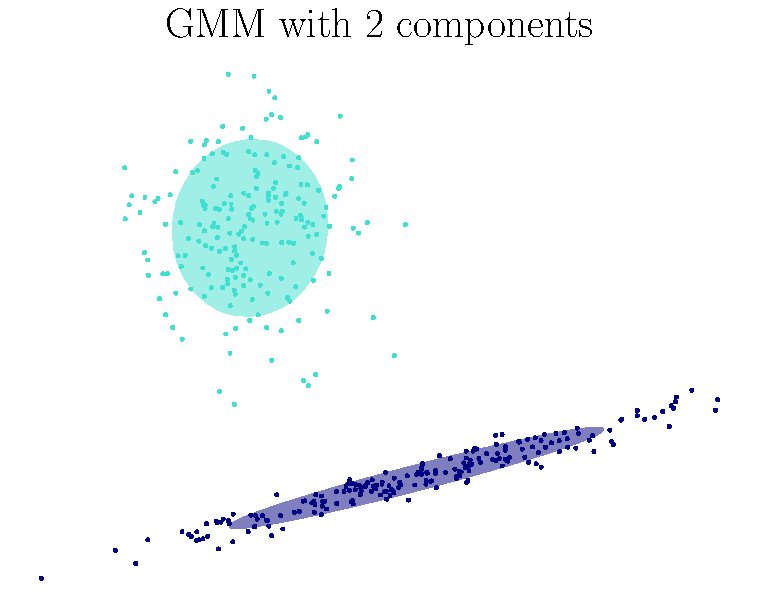
\includegraphics[page = 1, width=0.49\textwidth]{./figures/gmm}
\caption{Gaussian mixture model with two components. The equal probability surfaces are highlighted in colours.}
\label{fig:gmm}
\end{figure}
%------------------------------------------------------------

\section{Deep Generative Models}\label{sec:DGM}
We may regard the GMM as the simplest form of statistical generative model. Recent years have seen the advent of novel methods for generative modelling which we collectively refer to as Deep Generative Models (DGM), in complete analogy to what deep learning means with respect to machine learning. 
Before describing the most relevant forms of DGMs, and with no claim of completeness, we recall that some of the key features of deep learning include
\begin{itemize}
\item
models are parametrized by Neural Networks (NN) whose specific form depends on the particular task;
\item
the NN parameters are inferred via a stochastic gradient descent approach;
\item
in order to really exploit NNs, vast amount of high-fidelity data is needed for their training.
\end{itemize}
The last bullet is particularly attractive for LHC analysis, in that not only scientific collaborations such as ATLAS and CMS have already collected petabytes of data (with a lot more to come with the next upgrade of the collider), but we can also prepare data in a controlled environment for benchmarking models.

Concerning the practical realisation of DGMs, the three most successful frameworks studied and employed in the literature are
\begin{itemize}
\item
Normalizing Flows (NF~\cite{inn,coupling2,glow, nflow1,papamakarios2019normalizing,nflow_review,mller2018neural, grathwohl2018ffjord,chen2019neural});
\item
Generative Adversarial Networks (GAN)~\cite{goodfellow,Creswell2018, wgan_gp, wgan_original, lim2017geometric, zhang2019selfattention};
\item
Variational Autoencoders~\cite{kingma2014autoencoding,Kingma2019}.
\end{itemize}
The first two have been extensively employed in this thesis, and will be therefore further elaborated in the following sections.

\subsection{Normaling Flows}\label{intro:normflow}
Normalizing Flow  are defined in terms of a parametrized change of variable $G_{\theta}: z \rightarrow x$ between distributions
%
\begin{align}\label{eq:nf}
p_X(x) = p_Z(z) \left|\det \frac{\partial G_{\theta}(z)}{\partial z}\right|^{-1} = p_Z(\bar{G}_{\theta}(x)) \left|\det \frac{\partial \bar{G}_{\theta}(x)}{\partial x}\right|,
\end{align}
%
where $\bar{G}_{\theta} = G^{-1}_{\theta}$.
Regardless of how complicated $p_{X}(x)$ may be, if there exists a bijection $G_{\theta}$ such that $p_Z(z)$ is a simple distribution, e.g.\ a Gaussian $\mathcal{N}_{\mu=0, \Sigma=\mathbb{I}}$, we can draw samples from $p_{X}(x)$ via the generative pipeline
%
\begin{align}
z \sim p_Z(z) \longrightarrow x = G_{\theta}(z)  \sim p_{X}(x),
\end{align}
%
%
%------------------------------------------------------------
\begin{figure}[t]
\centering
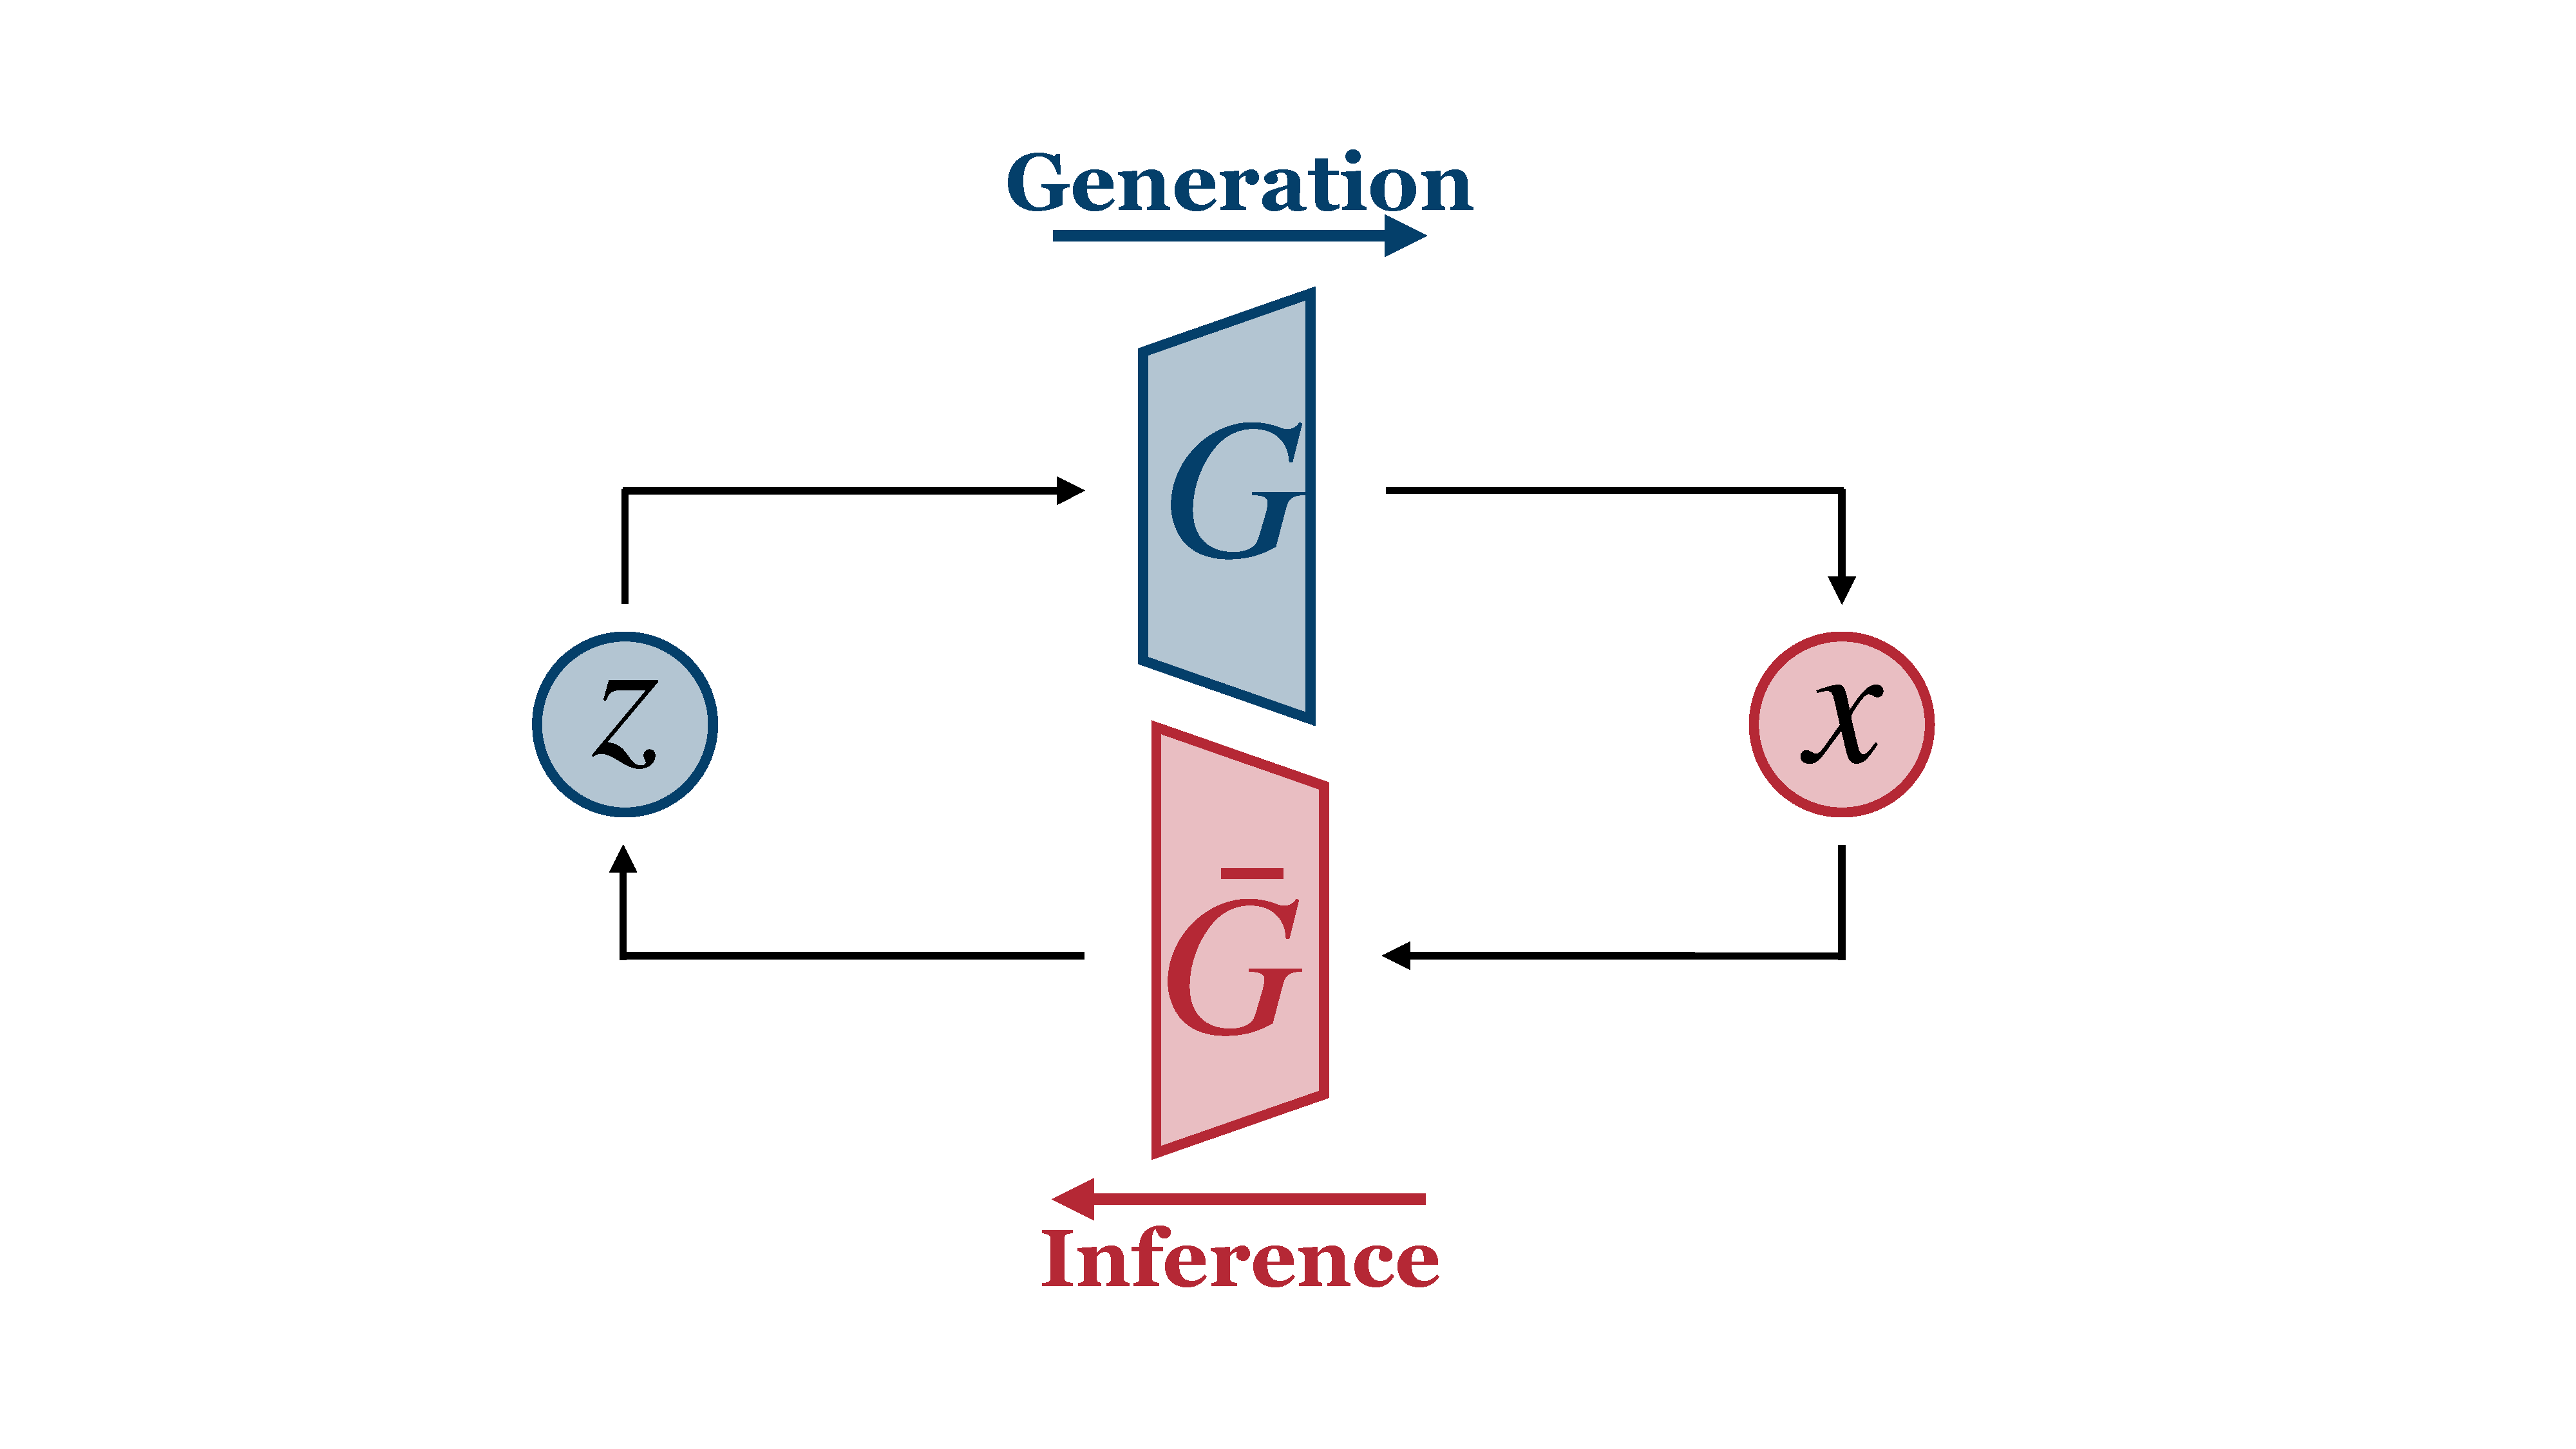
\includegraphics[page = 1, width=0.99\textwidth]{./figures/inn}
\caption{Schematic representation of a NF: a random variable $z$ sampled from a fixed, simple distribution is transformed via a map $G$ to a sample $x$ sampled from a complex target distribution. If $G$ is a bijection, and its inverse $\bar{G} = G^{-1}$ can be easily evaluated, the inverse direction can be used to train the model with Maximum Likelihood.}
\label{fig:NF}
\end{figure}
%------------------------------------------------------------
%
see Fig.~\ref{fig:NF} for a schematic representation. Similar to the GMM example in Sec.~\ref{sec:gmm}, the parameters of $G_{\theta}$ can be chosen to minimize the negative log-likelihood
%
\begin{align}\label{eq:change_of_variable}
\begin{split}
\mathcal{L} &= - \sum_{n=1}^N \log \left[ p_Z(\bar{G} _{\theta}(x_n)) \left|\det \frac{\partial \bar{G} _{\theta}(x)}{\partial x_n}\right| \right]\\
&= -\sum_{n=1}^N \log p_Z(\bar{G} _{\theta}(x_n)) + \log \left|\det \frac{\partial \bar{G} _{\theta}(x_n)}{\partial x_n}\right|\\
&= \sum_{n=1}^N \frac{(\bar{G} _{\theta}(x_n))^2}{2} - \log \left|\det \frac{\partial \bar{G} _{\theta}(x_n)}{\partial x_n}\right|,
\end{split}
\end{align}
%
where we have used $p_{Z}(z) = \mathcal{N}_{\mu=0, \Sigma=\mathbb{I}}$ and have discarded irrelevant constant terms. 
In practice, we only need to compute $\bar{G} _{\theta}(x_n)$, the corresponding determinant of the Jacobian, and minimize the combination in the final line of Eq.~\ref{eq:change_of_variable}.

This rather straightforward blueprint hides three complications one needs to carefully address. First of all, not only $G_{\theta}$ must be a bijection, i.e.\ its inverse must exist, but both $G_{\theta}$ and $\bar{G} _{\theta}$ must be efficiently computable, as one is required for training and the other for generating. Finally, the map must have a tractable Jacobian. If $G_{\theta}$ is parametrized by a standard NN, such as a Multi-Layer Perceptron (MLP), none of the three properties is satisfied. These constraints restrict the class of allowed transformations, limiting the expressive power at our disposal.
However, not all hope is lost, as we can build progressively more complex maps by simply stacking many simple functions, while maintaining the tractability of the Jacobian.
Given a bijection $G_{i}$ with inverse $\bar{G}_{i}$ and a cheap Jacobian, the composition
\begin{align}
G = G_{n} \cdot  G_{n-1} \ldots \cdot G_{1}
\end{align}
has inverse
\begin{align}
\bar{G} = \bar{G}_{1} \cdot   \ldots \cdot \bar{G}_{n-1} \cdot \bar{G}_{n},
\end{align}
and its determinant is the product of each individual determinant
\begin{align}
\det G = \prod_{i=1}^{N}  \det G_{i}.
\end{align}
This means that a composition of bijections is again a bijection whose computational complexity simply grows linearly with the number of compositions.
As a result, this research line is primarily dedicated to finding the optimal trade-off between computational complexity and model expressive power. 
In the remaining of this section we give an overview of past and currently used methods.

\subsubsection{Planar and Radial Flows}
The original work on NFs~\cite{pmlr-v37-rezende15} introduces the simple planar and radial flows. Despite representing seemingly simple transformations, they are not easily invertible.
A planar flow takes the form
%
\begin{align}
G(x) = x + u h(w^{T}x + b),
\end{align}
%
where $u, w, b$ are parameters and $h$ is a non-linear activation function. This transformation expands and contracts the distribution of $x$ along certain axis. The planar flow has the simple Jacobian
%
\begin{align}
\det \frac{\partial G}{\partial x} = 1 + h^{'}(w^{T}x + b) u^{T}w
\end{align}
%
which can be computed in $\mathcal{O}(D)$ time but cannot be inverted in closed form and its inverse does not exist in general.
Radial flows modify instead the distribution around a point $x_0$ as
%
\begin{align}
G(x) = x + \frac{\beta}{\alpha + ||x - x_0||}(x - x_0).
\end{align}
%
The same considerations apply here, the determinant of a radial flow can be efficiently computed, but its inverse is not always defined and cannot be computed in closed form.

\subsubsection{Dimensional Partitioning}

Introduced in ~\cite{coupling1, coupling2}, this approach builds an invertible transformation by splitting a $D$-dimensional input $x$ into two subspaces $(x_1, x_2)$, and defining the bijection $G$, normally called a coupling layer, as
%
\begin{align}
y_1 &= h(x_1, f(x_2))\\
y_2 &= x_2.
\end{align}
%
with inverse
%
\begin{align}
x_1 &= h^{-1}(y_1, f(y_2))\\
x_2 &= y_2.
\end{align}
%
The main feature of a coupling layer is that even if $f$ is an arbitrary function, the Jacobian of $G$ is always a triangular matrix which does not depend on the derivative of $f$. 
Different strategies can be used to perform the partitioning and ensure that every 
dimension gets transformed, such as alternating splittings in half and random 
permutations~\cite{coupling1}, using masked flow~\cite{coupling2} or using $(1 \times 1)$ convolutions~\cite{glow}. 
This is the method of choice for all the studies in this thesis, and in Chap.~\ref{chap:unfolding} we explain in details our implementation. 

\subsubsection{Autoregressive Flows}

An autoregressive flow is a non-linear generalization of a multiplication by a triangular matrix~\cite{kingma2017improving, papamakarios2018masked}. 
Motivated by the product rule of probability, stating that a joint density can be computed as a product of one dimensional conditionals
%
\begin{align}
p(x) = \prod_i p (x_i | x_{1:i-1}),
\end{align}
%
in an autoregressive model the output $y = G(x)$ is computed step-by-step as a function conditioned on the previous entries, i.e.\   
%
\begin{align}
y_t = h(x_t, f_t(x_{1:t-1})),
\end{align}
%
where $x_{1:t} = (x_1, \ldots, x_t)$, and $f_t$ is an arbitrary map taking a $t-1$ dimensional input. 
Similarly to a coupling layer, since each output $y_t$ only depends on $x_{1:t}$, the resulting Jacobian is again triangular and its determinant can be efficiently computed. The main difference with respect to coupling layers is that the inverse function, which can be trivially computed for the former, must be computed recursively as
%
\begin{align}
x_t = h^{-1}(y_t, f_t(x_{1:t-1})).
\end{align}
%
As this operation is inherently sequential, it cannot be parallelized and represent therefore a bottleneck for training this kind of model. Depending on the application, one may want to either have a fast forward direction, in which case one gets a so called masked autoregressive flow, or a fast inverse direction, giving instead an inverse autoregressive flow.

\subsubsection{Residual Flows and ODE}

The last method we present is based on residual connections, i.e.\  maps with the form
%
\begin{align}
G(x) = x + f(x).
\end{align}
%
Residual blocks have been used for a long time~\cite{he2015deep}, and have been adapted into invertible architecture in Ref.~\cite{gomez2017reversible, jacobsen2018irevnet}. Splitting input and output as $(x_1, x_2)$, $(y_1, y_2)$, the map
%
\begin{align}
y_1 &= x_1 + f(x_2)\\
y_2 &= x_2 + l(y_1)
\end{align}
%
is trivially invertible, but has an inefficient Jacobian. Ref.~\cite{gomez2017reversible, jacobsen2018irevnet} introduces
strategies to enforce the invertibility.
Most notably, however, is the fact one can see a residual connection as the discretized 
version of an ordinary differential equation. 
The starting point is an ordinary differential equation of the form
%
\begin{align}\label{eq:ode}
\frac{d}{dt}x(t) = F(x(t), \theta(t)),
\end{align}
%
where $F : \mathbb{R}^D \times \Theta \rightarrow \mathbb{R}^D$ encodes the dynamics of the system, $\Theta$ is a set of parameters and $\theta : \mathbb{R} \rightarrow \Theta$ is a parametrization.
The discrete version of Eq.~\ref{eq:ode} 
%
\begin{align}
x_{n+1} - x_n = \epsilon F(x_n, \theta_n), 
\end{align}
%
is equivalent to the equation of a residual connection with residual block $\epsilon F$.
Starting from this intuition, Ref.~\cite{dupont2019augmented, chen2019neural , grathwohl2018ffjord} 
propose to directly solve the continuous version Eq.~\ref{eq:ode}, which in this differential equation picture 
would correspond to training an infinitely deep network.

\medskip

We conclude this section with a comment motivating the study of Chap.~\ref{chap:lsr}. As already stated, invertible models are bijections, or homeomorphisms~\cite{dupont2019augmented,  huang2020augmented} (note that this is a strict equivalence, i.e.\   an invertible model does not approximate a homeomorphism, it is one), and as such they are by construction unable to map manifolds with different topological features, such as the number of holes and disconnected patches. In particular, if we stick to the standard formulation and only consider Gaussian latent spaces, we may only be able to represent data whose underlying manifold is compact and has genus zero. As this may be a limiting factor for the naive use of normalizing flows in particle physics, in Chap.~\ref{chap:lsr} we illustrate a possible method to account for it.

\subsection{Generative Adversarial Networks}\label{intro:gan}
GANs introduce a brand new paradigm for generative modelling which, unlike the previously described methods, doesn't involve computing the likelihood at all, and is therefore a form of likelihood-free machine learning. Instead, GANs rely on a two-sample test between distributions, i.e.\   a statistical test to determine whether or not two samples are drawn from the same distribution. This test is formulated as a differentiable objective function so that it can be minimized with stochastic gradient descent methods, in such a way that it is minimal iff the two distributions are statistically identical.
The statistical test is performed by a discriminator $D_{\phi}$ whose job is to tell apart real and fake samples. The final piece of a GAN is a generator $G_{\theta}$, a map from noise $z$ to target samples $\tilde{x}$, see Fig.~\ref{fig:gan}. In DL, both $D_{\phi}$ and $G_{\theta}$ are properly shaped NNs.
%
%------------------------------------------------------------
\begin{figure}[t]
\centering
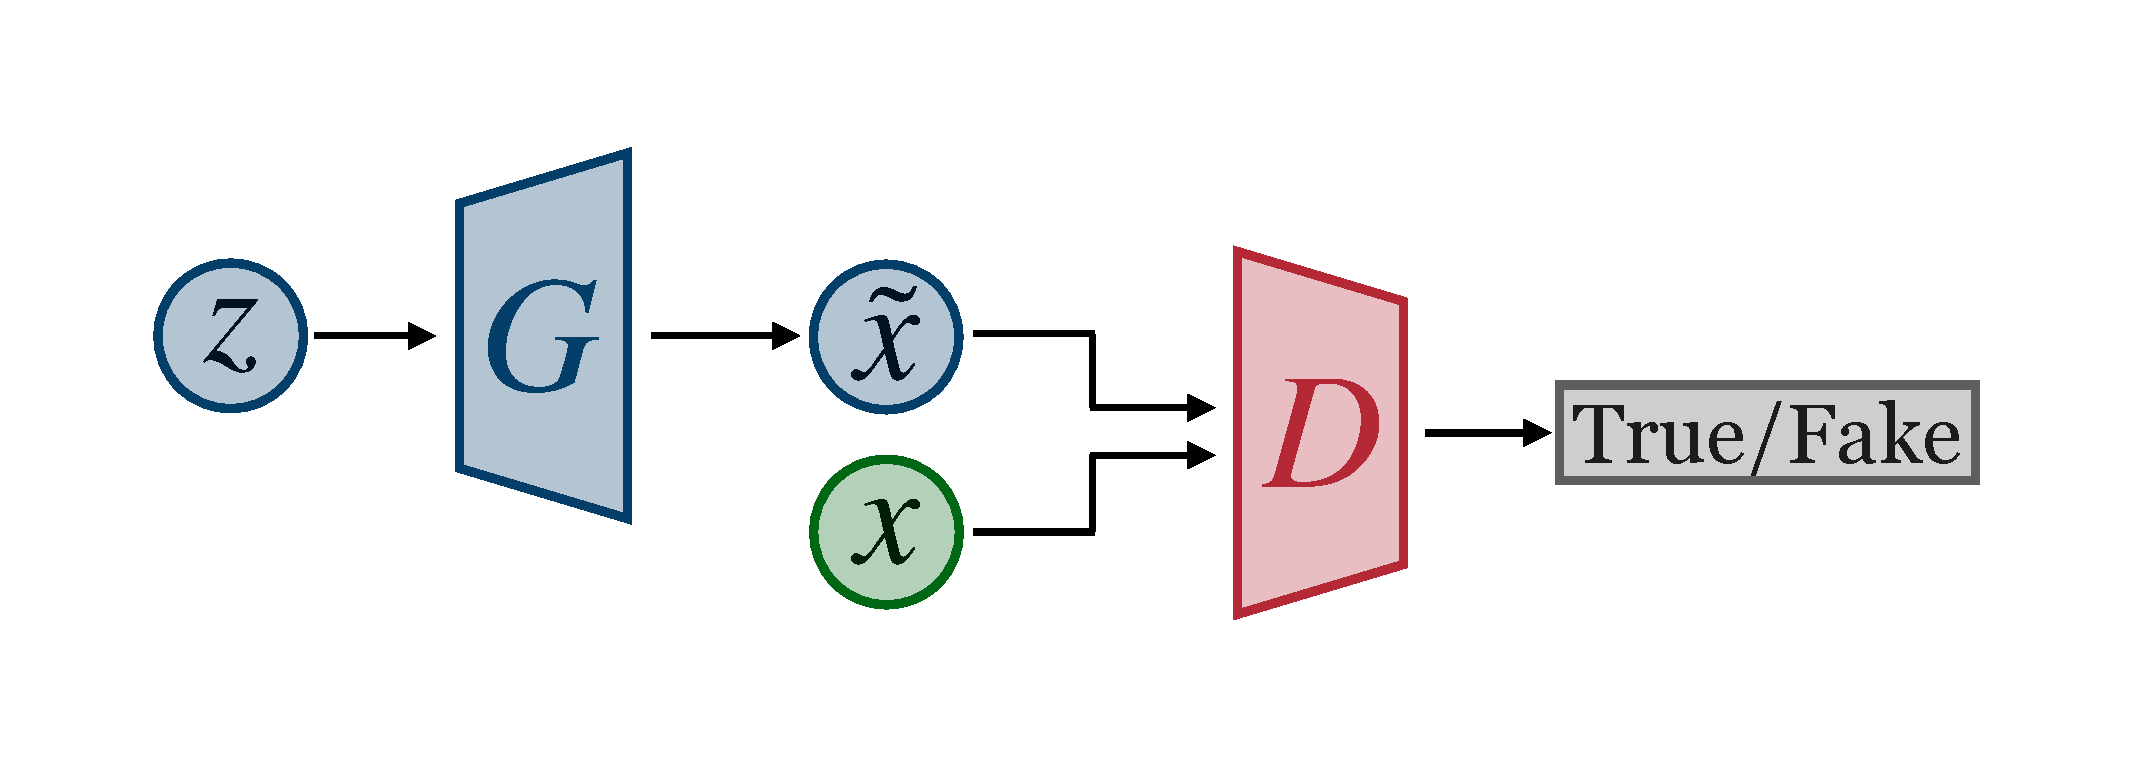
\includegraphics[page = 1, width=0.99\textwidth]{./figures/gan}
\caption{Schematic representation of a GAN: a generator $G$ deterministically maps noise $z$ to fake samples $\tilde{x}$. The discriminator $D$ is trained as a binary classifier of true versus fake data, while $G$ tries to fool it.}
\label{fig:gan}
\end{figure}
%------------------------------------------------------------
%
While many different ways to define the GAN objective have been proposed, we refer to the original formulation\cite{goodfellow} as it is close to the one employed in Chap.~\ref{chap:unfolding}. Formally, we consider the min-max game 
%
\begin{align}
\min_{\theta} \max_{\phi}\mathbb{E}_{x \sim p_{X}(x)} \left[ \log D_{\phi} (x) \right] + \mathbb{E}_{z\sim p_{Z}(z)} \left[ \log \left( 1 - D_{\phi} (G_{\theta}(z) \right) \right].
\end{align}
%
For a fixed generator, this is nothing other than a binary classification task, and an optimal discriminator should output $1$ for any $x \sim p_{X}(x)$ and $0$ otherwise, which we can summarize as
%
\begin{align}
D_{\phi^{*}}(x) = \frac{p_{X}(x)}{p_{X}(x) + p_{G}(x)},
\end{align}
%
with $p_{G}(x)$ being the distribution implicitly defined by the generator. 
Fixing $\phi = \phi^{*}$, the generator part of the objective is equivalent to minimizing the Jenson-Shannon divergence $JS(p_{X}, p_{G})$, with
%
\begin{align}
JS\left(p, q\right) = \frac{1}{2} \left(KL\left(p, \frac{p + q}{2}\right) + KL\left(q, \frac{p + q}{2}\right) \right),
\end{align}
%
and $KL(a, b)$ is the Kullback-Leibler divergence between $p$ and $q$. This objective has a global minimum for $p_{G} = p_{X}$.
It turns out that if the discriminator is optimal, the objective function has vanishing gradient for the generator, leading to the standard alternating training of GANs: every $k$ updates of $\phi$ we perform an update of $\theta$, $k$ being a hyperparameter.
Training a GAN is a highly non trivial task with many potential issues if extra care is not taken, notably
\begin{itemize}
\item
the optimization procedure is typically unstable and needs to be regularized;
\item
for multi-modal targets, generators can collapse to a single mode;
\item
since the objective function is not convex, there is no clear way to evaluate the model performances or to determine a stopping point.
\end{itemize}
%Plenty of empirical tips and tricks to stabilize the training of GANs are available in the literature, in the form of modified objective functions, gradient penalties, noise injection, specific optimizers and more.

An important difference between the two presented frameworks is that a GAN represents a target density only implicitly, i.e.\    $G_{\theta}$ is only a sampler from $p_{X}$, but can't be used to estimate its value (with the exception of low dimensional problems where kernel methods may be used to smooth a binned distribution). On the other hand, the explicit value of the density can be trivially computed with a NF from Eq.~\ref{eq:nf} if we assume a perfect map to the latent space distribution.

\section{Unfolding}\label{intro:unfolding}

In any quantitative science we wish to be able to estimate the possible value of "true" parameters, directly connected to some underlying theory, given that we are only able of observing a distorted version of them in the best scenario, more realistically we will have to be satisfied with observing a different set of parameters entirely.
In particular, we are often interested in lifting the effects induced by the detectors and possible physical and theoretical backgrounds. This procedure is normally called de-convolution, and takes the name of unfolding in particle physics. In this section we first revise a standard method for unfolding based on Bayesian inference, and then illustrate how to set-up a deep-learning version of it.

\subsection{Iterated Bayesian Unfolding}
In this section we will define the fundamental ideas of unfolding following closely Ref.~\cite{DAgostini:1994fjx, dagostini2010improved}.
Bayesian inference is a framework to estimate unknown parameters from observed data. A starting point for Bayesian unfolding is the discretization of the problem, in the form of binning of observable distribution of events, with each bin being treated as an independent variables.
%
%------------------------------------------------------------
\begin{figure}[t]
\centering
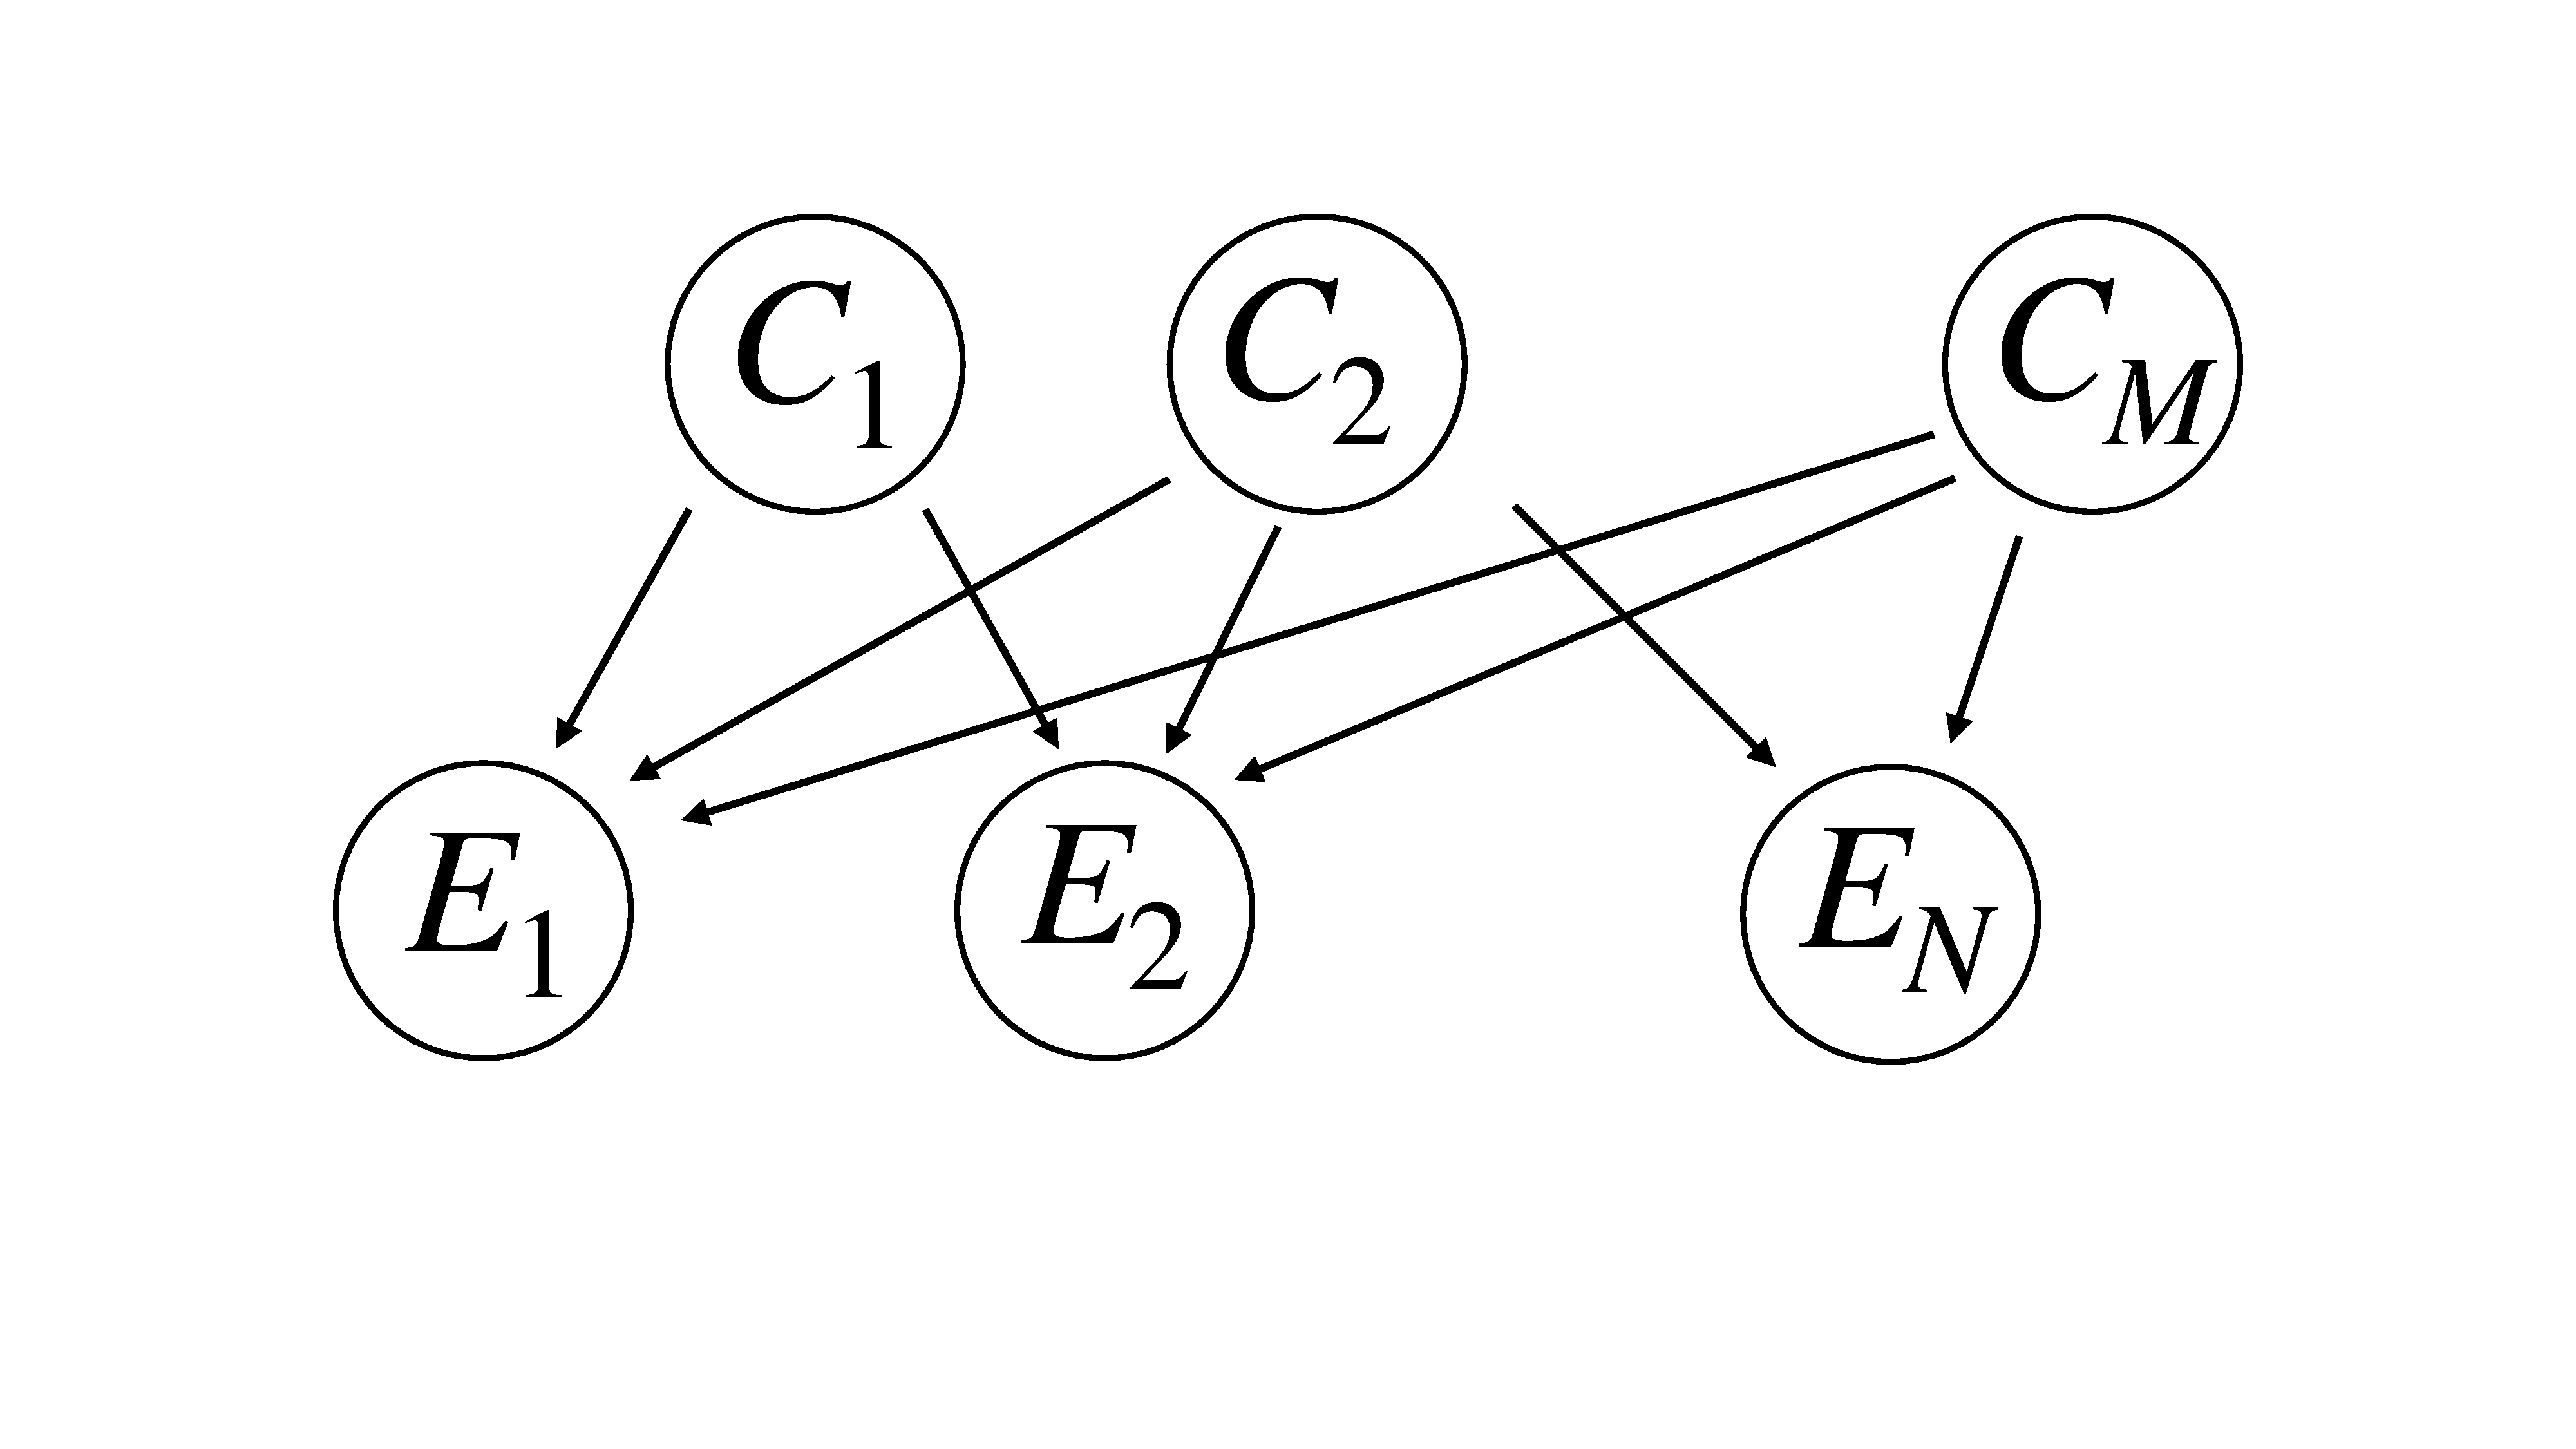
\includegraphics[page = 1, width=0.95\textwidth]{./figures/graphical_model}
\caption{Graphical model of causes and effects. Each arrow represents a probabilistic link}
\label{fig:graph_model}
\end{figure}
%------------------------------------------------------------
%
Borrowing the language of graphical models, the problem can be described by the Bayesian network of Fig.~\ref{fig:graph_model}, $C_{i}$ being the true number of events in each cause bin, given that we observe $E_{j}$ events per bin.
It's important to notice that as the links between cause and effect is probabilistic, so will be the number of true events per bin. Concretely,  given causes $C_i$ and effects $E_j$, we wish to estimate the conditional distribution
%
\begin{align}\label{eq:unf}
P(C_i | E_j)
\end{align}
%
Following standard Bayesian inference, Eq.~\ref{eq:unf} may be computed as
%
\begin{align}\label{eq:bayes_inf}
P(C_i | E_j) = \frac{P(E_j | C_i) P(C_i)}{\sum_{l=1}^{n_E} P(E_j| C_l) P(C_l)},
\end{align}
Eq.~\ref{eq:bayes_inf} is Bayes' theorem stating that the posterior is proportional to the likelihood, provided that we multiply by the prior
%
\begin{align}
P(C_i | E_j) \propto P(E_j | C_i) P(C_i),
\end{align}
%
and the denominator is a normalization factor.
%The main issue in the practical application of Eq.~\ref{eq:bayes_inf} is that there is no closed to compute 
The unfolding algorithm proceeds as follows:
\begin{itemize}
\item
estimate the number of expected events in bin $C_i$ given that $n(E_i)$ is the observed counting bin $E_j$\\
\begin{align}
n(C_i)|_{n(E_j)} \sim P(C_i | E_j) n(E_j);
\end{align}
\item
include effects from all observations\\
\begin{align}
n(C_i) = \sum_j P(C_i | E_j) n(E_j);
\end{align}
\item
correct for the effect of different efficiencies $\epsilon_i$\\
\begin{align}\label{eq:IBU}
\tilde{n}(C_i) = \frac{1}{\epsilon_i} n(C_i) = \frac{1}{\epsilon_i}\sum_{j=1}^{n_E} P(C_i | E_j) n(E_j);
\end{align}
with the efficiencies computed from the smearing matrix as
\begin{align}
\epsilon_i = \sum_{j=1}^{n_E} P(E_j | C_i) = \sum_{j=1}^{n_E} \lambda_{ij},
\end{align}
where $\lambda_{ij} = P(E_j | C_i)$ are the entries of a smearing matrix $\Lambda$ estimated from Monte Carlo simulations. 
\end{itemize}

The above algorithm is essentially the first form of Bayesian unfolding presented in Ref.~\cite{DAgostini:1994fjx}. Ref.~\cite{dagostini2010improved} introduced several improvements over the first version. A first improvements concerns the explicit modelling of the smearing matrix. In the original formulation, one starts by generating a large number of events in each cell and counting where they end up after the simulation. The entries $\lambda_{ij}$ are estimated as
%
\begin{align}
\lambda_{ij} \sim \frac{n(E_j)^{MC}}{n(C_i)^{MC}}.
\end{align}
%
We can both improve this estimate, and include its uncertainty, by employing again Bayes theorem and computing a posterior over the $\lambda_{ij}$. Given a column $\lambda_i$ of $\Lambda$, we have
%
\begin{align}
f(\lambda_i | n(E)^{MC}, n(C_i)^{MC}) \propto P(n(E)^{MC} | n(C_i)^{MC}, \lambda_i) f(\lambda_i).
\end{align}
%
If we choose a Dirichlet prior for $\lambda_i$ it is possible to show
%
\begin{align}
\lambda_i \sim \text{Dir}(\alpha_{\text{posterior}, i}), \quad \alpha_{\text{posterior}, i } = \alpha_{\text{prior}, i} + n(E)^{MC}|_{n(C_i)^{MC}},
\end{align}
%
where
%
\begin{align}
\text{Dir}(x | \alpha) = x_1^{\alpha_1 -1 } \ldots x_n^{\alpha_n -1 }.
\end{align}
%
We can now account for the extra uncertainty in $P(C_i | E_j)$ by computing
%%
%\begin{align}
%f(x | \alpha) = \frac{\Gamma(\alpha_1 + \ldots + \alpha_n)}{\Gamma(\alpha_1) \ldots \Gamma(\alpha_n)} x_1^{\alpha_1 -1} \ldots x_n^{\alpha_n -1}
%\end{align}
%%
%
\begin{align}
P(C_i | E_j) \longrightarrow P(C_i | E_j, \Lambda); \qquad P(C_i | E_j) = \int P(C_i | E_j) f(\Lambda) d\Lambda,
\end{align}
%
i.e.\ the posterior over causes depends explicitly on the smearing matrix $\Lambda$, which is sampled from the posterior distribution $f(\Lambda)$.
Most notably, however, is the additional iteration of the algorithm. Bayesian inference only makes sense when we have a prior belief of what the possible values of the unobserved parameters are. Choosing a "correct" prior is a tricky task, as this choice, which is arbitrary, affects the posterior distribution.
Ref.~\cite{dagostini2010improved} suggests that the dependence on the prior can be reduced by iterating the unfolding procedure, by using the result of unfolding step $n$ as the prior of unfolding $n+1$. This method is therefore called Iterated Bayesian Unfolding (IBU).

We conclude the introduction with a brief discussions of the limitations of iterated Bayesian unfolding, and equivalent methods. The first obvious limitation is that the method relies on binning measurements into histograms. Binning can be problematic as aside with the exception of few limited case there's no obvious best binning, and each individual observable typically requires an ad hoc manual choice of the binning. Directly related to this is the fact that the total number of bins grows exponentially with the number of dimensions, each being a different observable. This means that differential cross section measurements beyond a few dimensions are impractical.

\subsection{OmniFold}

In parallel to the work of Ref.~\cite{cond_gan, Bellagente:2020piv}, which constitutes the main content of Chap.~\ref{chap:unfolding}, another deep-learning framework for unfolding has been published. Because of its relevance as the only other existing method for unfolding relying on deep-learning, and for its connection to IBU, we believe that an explanation of the \textsc{OmniFold} method~\cite{Andreassen:2019cjw} deserves its own section.

\textsc{OmniFold} has been proposed to overcome the two main shortcomings of IBU, binning and handling multiple dimensions, by generalizing the iterated version of Eq.~\ref{eq:IBU} to the continuous, multi-dimensional case. In Fig.~\ref{fig:omnifold} we illustrate schematically the method.
%
%------------------------------------------------------------
\begin{figure}[t]
\centering
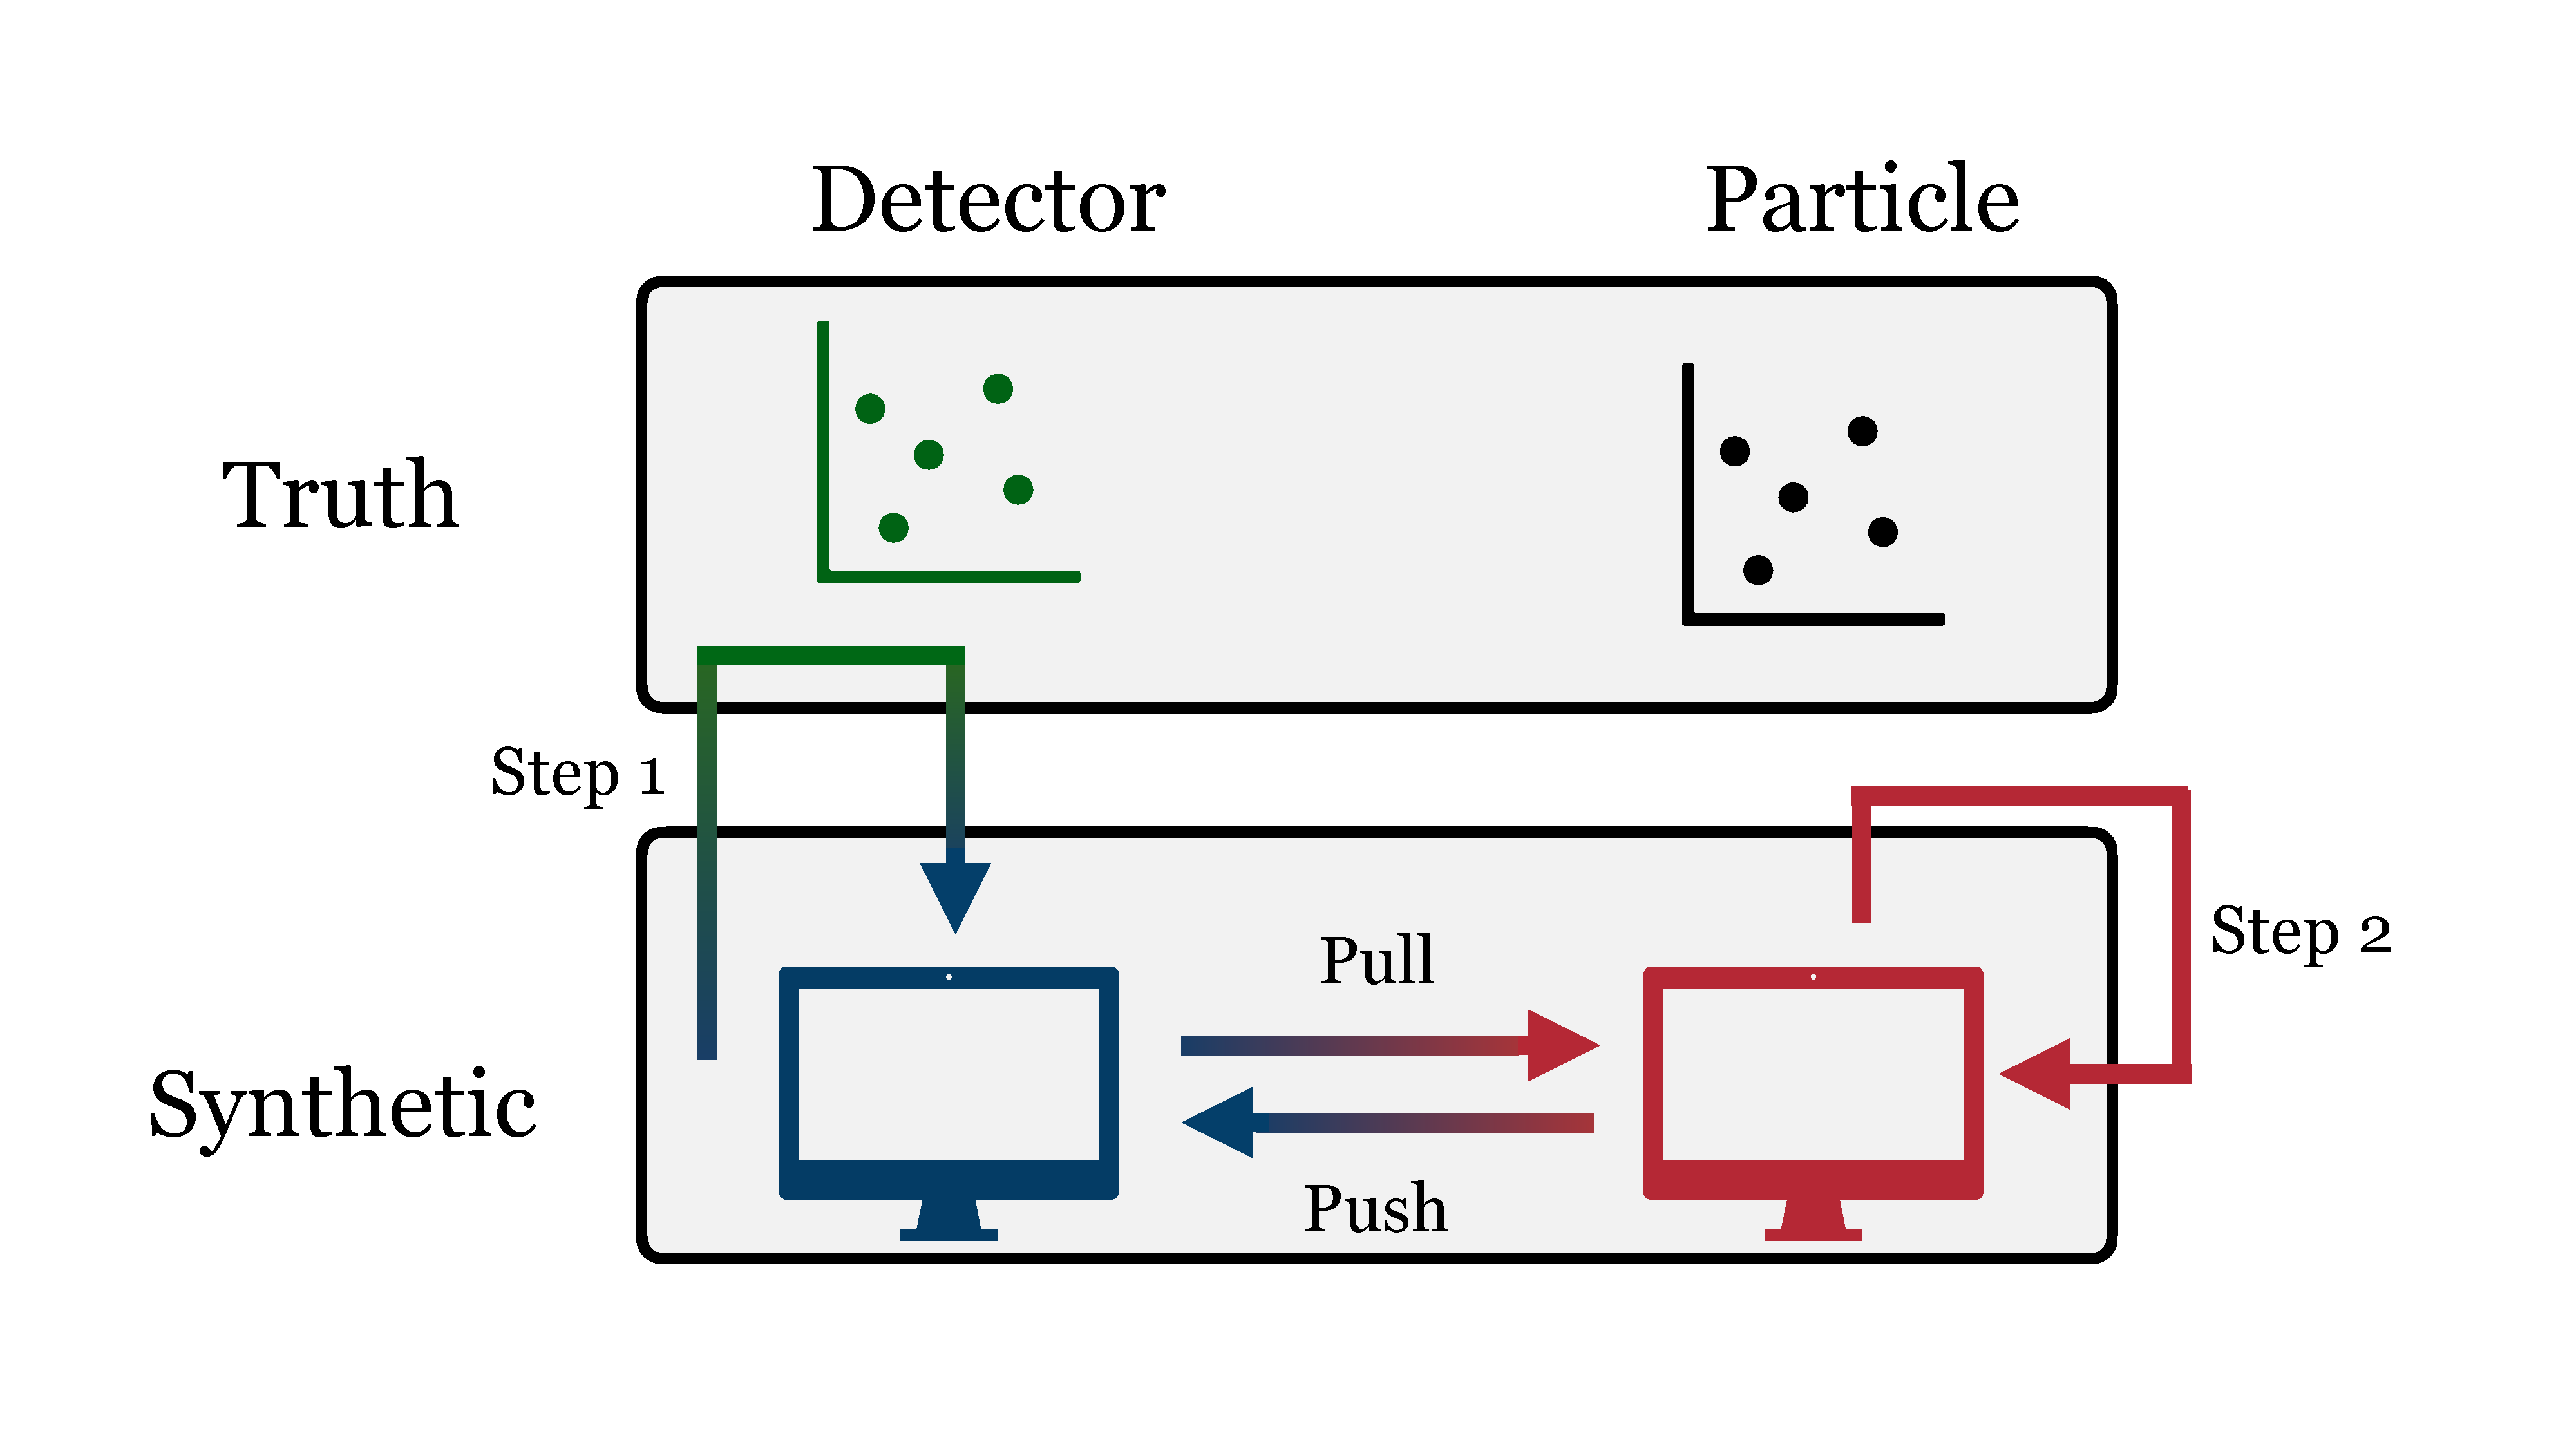
\includegraphics[page = 1, width=0.95\textwidth]{./figures/omnifold}
\caption{Illustration of the \textsc{OmniFold} method: synthetic data is reweighted against the true data at the detector level. This weights are pulled back at the particle level to induce weights on the particle level data. In the second step the original synthetic particle level data is weighted to match its reweighted version. The process is then iterated.}
\label{fig:omnifold}
\end{figure}
%------------------------------------------------------------
%
Starting with particle level events $t$ with initial weights $\nu_0(t)$ simulated with Monte Carlo, we produce a paired set of detector level events $m$ with induced weights $\nu_0^{\text{push}}(m) = \nu_0(t)$.
We then compute new weights $\omega_0(m)$, and use them to obtain the next set of particle level weights $\nu_1(t)$. The key idea to achieve the correct reweighting is that the likelihood ratio
%
\begin{align}
L \left[ (w, X), (w^{'}, X^{'}) \right](x) = \frac{p_{w, X}(x)}{p_{w^{'}, X^{'}}(x)},
\end{align}
%
can be approximated using a classifier trained to distinguish $(w, X)$ against $(w^{'}, X^{'})$~\cite{Andreassen:2019nnm, brehmer1, brehmer2, mining, cranmer2016approximating}.
With the likelihood ratio it is straightforward to reweight events as
\begin{align}
\omega_n(m) = \nu_{n-1}^{\text{push}} L \left[ (1, \text{truth, det)}), (\nu_{n-1}^{\text{push}}, \text{Synt, det)})\right],\\
\nu_n(t) = \nu_{n-1} L \left[ (\omega_n, \text{synt, part)}), (\nu_{n-1}, \text{synt, part)})\right].
\end{align}
It is possible to show that after one iteration the new weights are given by
%
\begin{align}
\nu_1 p_{synt, part}(t) = \int dm^{'} p_{\text{ synt, part| Synt, Det}} (t | m^{'}) p_{\text{truth, det}}(m^{'})
\end{align}
%
which is a continuous version of Eq.~\ref{eq:IBU}. On top of that, \textsc{OmniFold} is not limited by the dimensionality of the observables, and can in principle unfold the full phase space of an event, provided that the classifier employed is powerful enough.
%\input{inputs/B_SM.tex}
%\input{inputs/C_ML.tex}
%\input{inputs/L_GAN.tex}
%\input{inputs/M_PIML.tex}
%\input{inputs/N_PIML2.tex}
%\input{inputs/O_summary.tex}
%\clearpage
%\cleardoublepage
%\newpage
%\phantomsection
%\addcontentsline{toc}{chapter}{Acknowledgments}
%\chaptermark{Acknowledgments}
%\input{inputs/Z_danksagung.tex}
%\cleardoublepage
%%%%%%%%%%%%%%%%%%%%%%%%%%%%%%%%%%%%%%%%%%%%%%%%%%%%%%%%%%%%%%%%%%%%%%%%%
\begin{appendices}
\chapter{Appendix: conditional GAN}\label{chap:fcga)app}
%\appendix
\section{Performance}
\label{sec:app1}

%------------------------------------------------------------
\begin{figure}[b!]
\centering
\includegraphics[page = 2, width=0.49\textwidth]{figures/cGAN/pull_full}
\includegraphics[page = 3, width=0.49\textwidth]{figures/cGAN/pull_full} \\
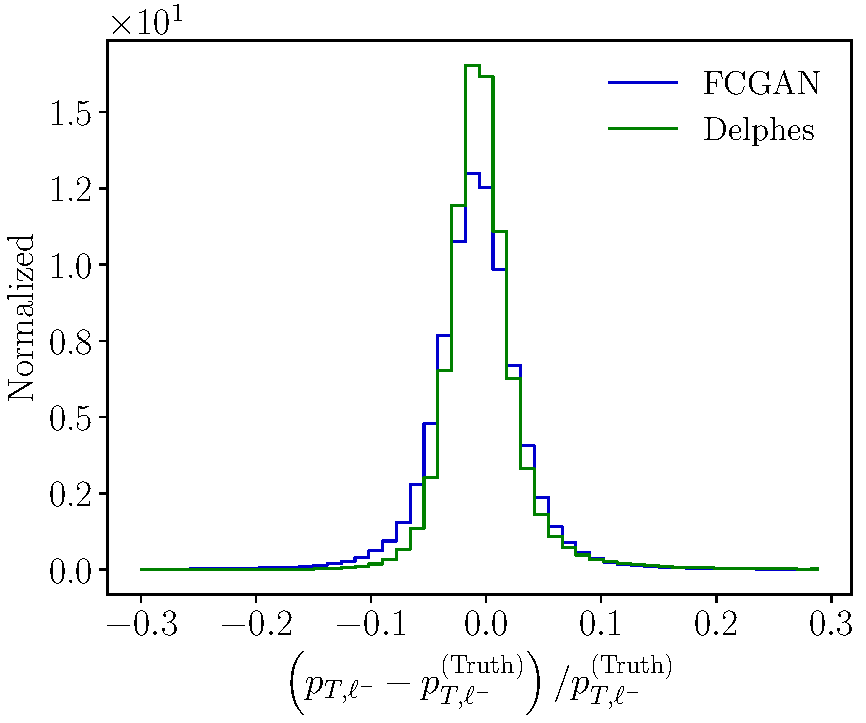
\includegraphics[page = 1, width=0.49\textwidth]{figures/cGAN/pull_full}
\includegraphics[page = 4, width=0.49\textwidth]{figures/cGAN/pull_full}
\caption{Normalized deviation between the FCGANned sample and truth (residual)
 for some of the kinematic variables.}
\label{fig:app_pull}
\end{figure}
%------------------------------------------------------------

While it is clear from the main text that the FCGAN inversion of the
fast detector simulation  works extremely well, we can still show some
additional standard measures to illustrate this. For instance, in
Fig.~\ref{fig:app_pull} we show the event-wise normalized deviation
between the parton-level truth kinematics and the \delphes and
FCGAN-inverted kinematics, for instance
%
\begin{align}
\frac{p_{T,j}^\text{(FCGAN)} - p_{T,j}^\text{(Truth)}}{p_{T,j}^\text{(Truth)}}
\qquad \text{and} \qquad
\frac{p_{T,j}^\text{(\delphes)} - p_{T,j}^\text{(Truth)}}{p_{T,j}^\text{(Truth)}} \; .
\end{align}
%
The events shown in these histograms correspond to the full phase
space inversion shown in Fig.~\ref{fig:distributions_FCGAN}, but from
the discussion in the main text it is clear that the picture does not
change when we invert only part of phase space.  As expected, we see
narrow peaks around zero, with a width in the $\pm 10\%$ range for the
jet momenta and much more narrow for the leptons, which are less
affected by detector smearing. For all distributions, but especially
the reconstructed $W$-mass, we see that the FCGAN reconstruction is
significantly closer to the parton-level truth than the \delphes
events are.

%------------------------------------------------------------
\begin{figure}[t]
\centering
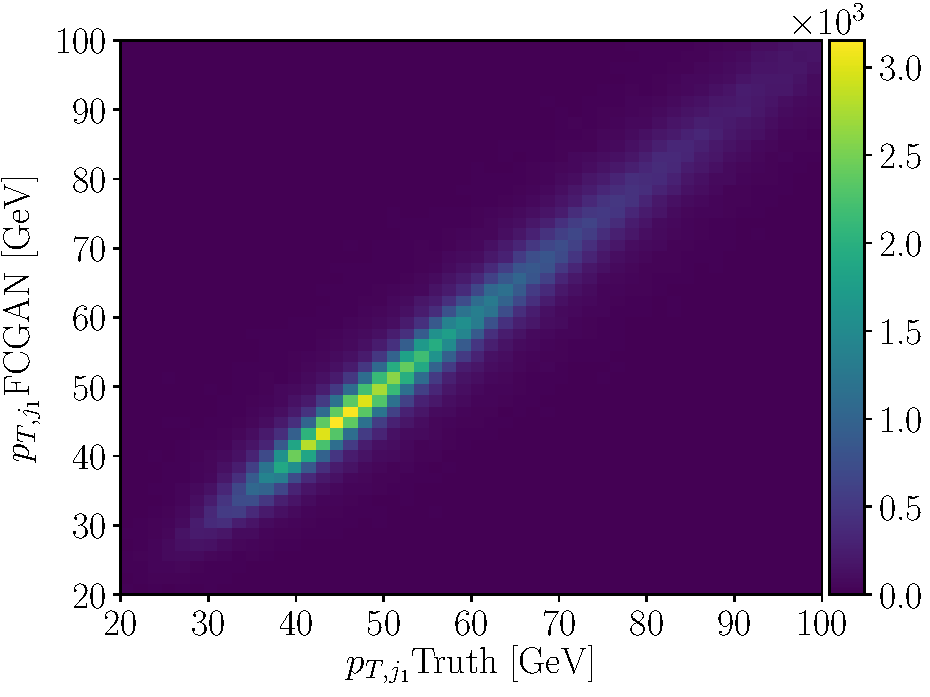
\includegraphics[page = 1, width=0.49\textwidth]{figures/cGAN/cGAN_pt1_corr}
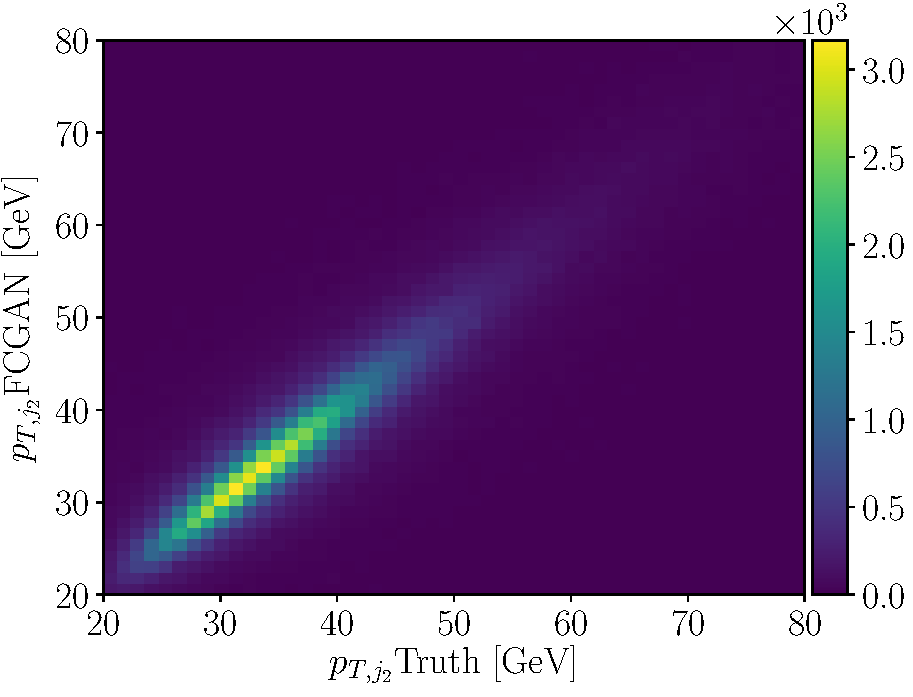
\includegraphics[page = 1, width=0.49\textwidth]{figures/cGAN/cGAN_pt2_corr}
\caption{Correlations between the FCGAN-inverted and parton-level truth
 kinematics, or migration matrix.}
\label{fig:app_2d}
\end{figure}
%------------------------------------------------------------

Finally, we show the migration matrix or correlation between true
parton-level and reconstructed parton-level events in terms of some of
the kinematic variables in Fig.~\ref{fig:app_2d}. Not surprisingly,
we observe narrow diagonal lines.

%%%%%%%%%%%%%%%%%%%%%%%%%%%%%%%%%%%%%%%%%%%%%%%%%%%%%%%%%%%%%%%%%%%%%%%%
\section{Staggered vs cooling MMD}
\label{sec:app}

The MMD loss is a two-sample test looking at the distance between
samples $x$, $x'$, drawn independently and identically distributed, in
terms of a kernel function $k\left(x, x'\right)$.  Implementations of
such a kernel, as given in Eq.~\ref{eq:kernels}, include a fixed
width or resolution $\sigma$.  We employ the MMD loss to reproduce the
invariant mass distribution of intermediate on-shell particles
$M_p$. A natural choice of $\sigma$ is the corresponding particle
width. However, this is inefficient at the beginning of the training,
when any generated invariant mass $M_G$ is essentially a random
uniform distribution. In that case $\left(x - x'\right)^2 \gg
\sigma^2$ for any $x, x' \sim M_G$, and Eq.~\ref{eq:MMD} reduces to
%
\begin{align}
\text{MMD}\left(k; M_G,M_P\right) \simeq \sqrt{\langle k\left(y,y'\right)\rangle_{y,y' \sim M_P}} \simeq \text{const} \; ,
\end{align}
%
and provides little to no gradient.

This can be avoided by computing the MMD loss using multiple kernels
with decreasing widths, so that the early training can be driven by
wide kernels.  A drawback of this approach is that only the small
subset of kernels with a resolution close to the evolving width of
$M_G$ gives a non-negligible gradient.

Alternatively, we can employ a cooling kernel, which we initialize to
some large value and then shrink to the correct particle width. This
is an efficient solution at all stages of the training.  A subtlety is
that the rate of the cooling has to follow the pace of the
generator in producing narrower invariant mass
distributions. Ultimately, we want to avoid hand-crafting the cooling
process, because it adds hyper-parameters we need to tune.  We use a
dynamic kernel width as a fixed fraction of the standard deviation of
the $M_G$ distribution.  This standard deviation as an estimate of the
width of $M_{G}$ can be replaced by any measure of the shape of
$M_{G}$, such as the full width at half maximum, and our tests show
that the performance is largely insensitive to the choice of the
fraction.

Yet another approach is based on the observation that the MMD kernel
test is not restricted to one-dimensional distributions
~\cite{GMMN,MomentMatching, MMDgen}.
This allows us to improve the invariant mass reconstruction by including
 additional physical information $x_i$ to the test, so that the
 discrepancy is not computed just between the samples $M_P$ and $M_G$
 of real and generated invariant masses, but rather between
 $(M_P, x_P)$ and $(M_G, x_G)$.
In the FCGAN spirit we therefore augment the batches of true and
generated invariant masses with one of
conditional invariant masses. From the same detector
information used to condition the generator and the discriminator, we
can extract the detector level invariant masses $M_D$ and accordingly
compute $\text{MMD}(k; (M_G, M_D), (M_P, M_D))$. Even tough
this does not represent a conditional MMD, training with multiple
kernels benefits from using the augmented batches. In
Fig.~\ref{fig:kernels_comparison} we compare the same invariant mass
distribution using these different MMD implementations.

%-------------------------------------------------
\begin{figure}[t]
\centering
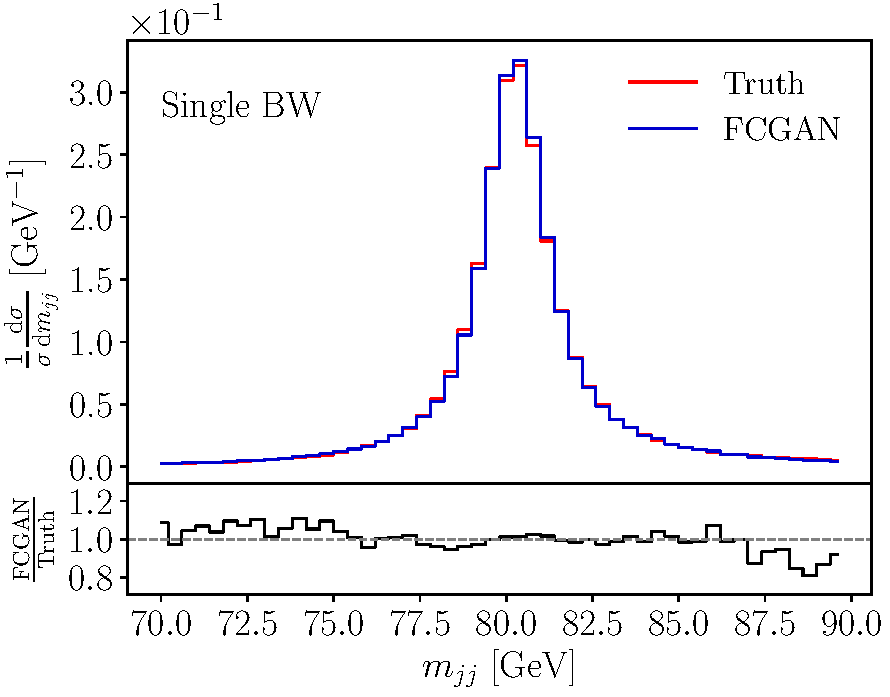
\includegraphics[page=1,width=0.49\textwidth]{figures/cGAN/single_1}
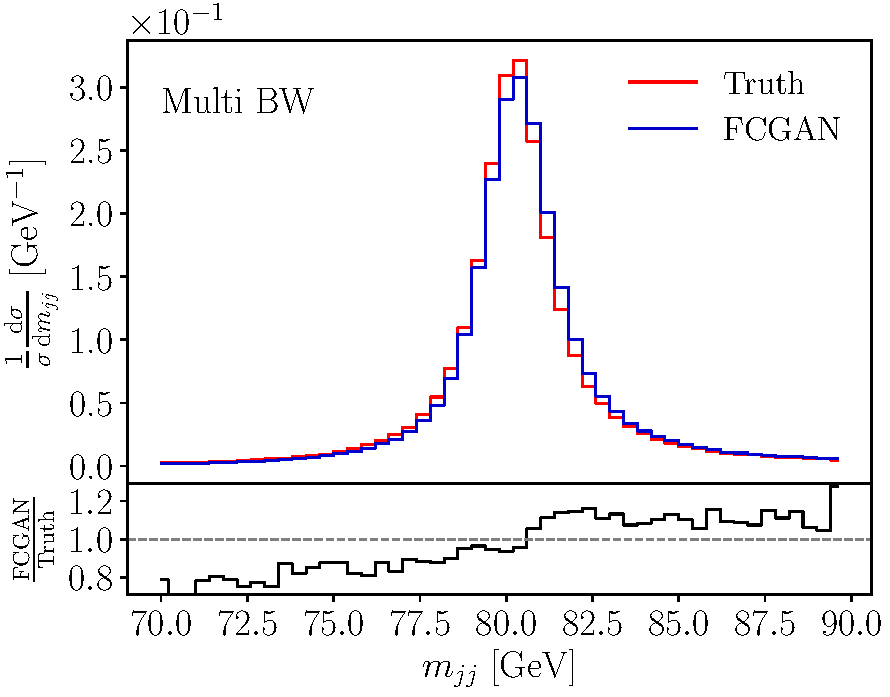
\includegraphics[page=1,width=0.49\textwidth]{figures/cGAN/multi_1}\\
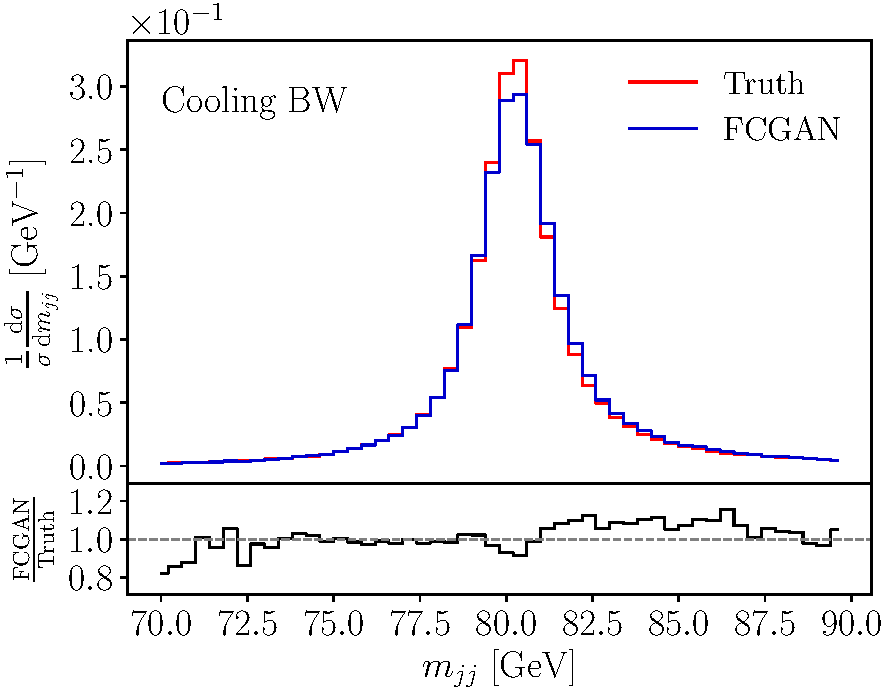
\includegraphics[page=1,width=0.49\textwidth]{figures/cGAN/cooling_1}
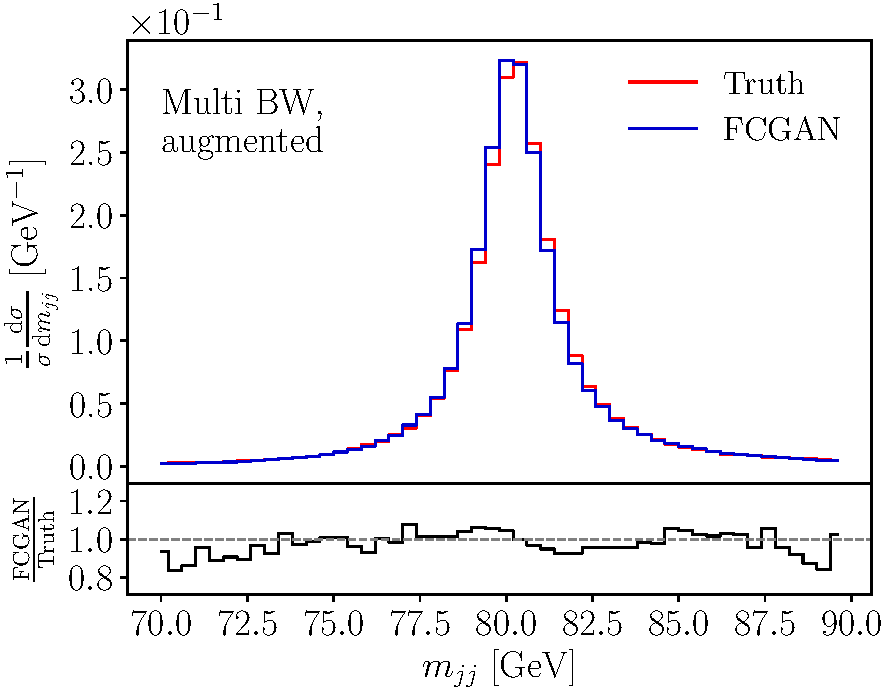
\includegraphics[page=1,width=0.49\textwidth]{figures/cGAN/combined_1}
\caption{Invariant jet-jet mass distribution for different MMD loss
  implementations: single kernel (upper left), multiple kernels (upper
  right), cooling kernel (lower left) and augmented multiple kernels
  (lower right).}
\label{fig:kernels_comparison}
\end{figure}
%-------------------------------------------------

\end{appendices}

%\documentclass[a4paper,twoside,10pt,openright]{report}%Dokumentenklasse 
\usepackage{graphicx} %Compiler

\usepackage{dsfont}

%%%% Schrift und Kodierung %%%%
	\usepackage[T1]{fontenc} %Zeichensatzkodierung von 7bit auf 8bit 
	\usepackage[utf8]{inputenc} %Zeichensatzkodierung Unicode bzw. UTF8
	\usepackage{lmodern} %Vektorschrift
	%\RequirePackage[english,spanish,es-nolayout]{babel}
	\usepackage[english]{babel}
	\usepackage{textcomp}
	\usepackage{lmodern}
	\usepackage{url}
	\usepackage[bookmarksnumbered=true]{hyperref}
    \graphicspath{{figures/}}	
	
%%% COLORS %%%
\newcommand{\hl}[1]{
   \textcolor{MidnightBlue!90!black}{#1} 
}

\usepackage{pifont}% http://ctan.org/pkg/pifont
\newcommand{\cmark}{\ding{51}}%
\newcommand{\xmark}{\ding{55}}%

\usepackage{stackrel}

\usepackage{feynmp}

\usepackage{amsthm}
\newtheorem{definition}{Definition}
\newtheorem{proposition}{Proposition}
	
%%%% Fancy Header %%%
\usepackage{fancyhdr}
\usepackage[dvipsnames]{xcolor}
\usepackage{tikz} 
\usepackage{pgfplots}
%\usepackage{pgf-pie}

\usetikzlibrary{arrows}
\usetikzlibrary{shapes.geometric, arrows}

\definecolor{mycolor}{rgb}{0.45,0.45,0.45}% dark grey

\newcommand{\mcD}{\mathcal{D}}
\newcommand{\mcL}{\mathcal{L}}
\newcommand{\dth}{\Delta_{\text{th/sys}}}
\newcommand{\dst}{\Delta_{\text{stat}}}
\newcommand{\dsy}{\Delta_{\text{syst}}}
\newcommand{\sthsy}{\sigma_{\text{th/sys}}}
\newcommand{\sth}{\sigma_{\text{th}}}
\newcommand{\sst}{\sigma_{\text{stat}}}
\newcommand{\ssy}{\sigma_{\text{syst}}}

\newcommand{\Langle}{\big\langle}
\newcommand{\Rangle}{\big\rangle} 
 
\fancyhf{}
\fancyhead[LE]{\sffamily\color{mycolor}\nouppercase{\leftmark}} % left even, right odd
\fancyhead[RO]{\sffamily\color{mycolor}\nouppercase{\rightmark}} % left even, right odd
\fancyfoot[CE,CO]{\sffamily\color{mycolor}\nouppercase{\thepage}} % center even, center odd
\renewcommand{\headrule}{{\color{mycolor}%
\hrule width\headwidth height\headrulewidth \vskip-\headrulewidth}}
\renewcommand{\headrulewidth}{0.5pt}

\fancypagestyle{plain}{%
    \fancyhf{}%
    \fancyfoot[CE,CO]{ { \sffamily\color{mycolor}{\thepage} } }
	\renewcommand{\headrulewidth}{0.0pt}
}

%\fancypagestyle{fancy}{%
%   \fancyhf{}
%	\fancyhead[LE,RO]{\sffamily\color{mycolor}\nouppercase{\leftmark}} % left even, right odd
%	\fancyfoot[CE,CO]{\sffamily\color{mycolor}\nouppercase{\thepage}} % center even, center odd
%	\renewcommand{\headrule}{{\color{mycolor}%
%	\hrule width\headwidth height\headrulewidth \vskip-\headrulewidth}}
%	\renewcommand{\headrulewidth}{0.5pt}
%}


%%% Customize titles %%%%
\usepackage[ ]{titlesec}  %
\usepackage{etoolbox}
\makeatletter
\patchcmd{\ttlh@hang}{\parindent\z@}{\parindent\z@\leavevmode}{}{}
\patchcmd{\ttlh@hang}{\noindent}{}{}{}
\makeatother
%\titleformat{\chapter}[display]
%  { \normalsize \huge  \color{black}}%
%  {\flushright \normalsize \color{mycolor} \MakeUppercase %
%  {\sffamily \chaptertitlename } \hspace{1 ex}%
%  { \fontsize{60}{60}\selectfont \color{mycolor} \sffamily  \thechapter }}%
%  {10 pt}%
%  {\sffamily \huge \color{mycolor}\bfseries}
%\newcommand\mychapformat[1]{\parbox[t]{\dimexpr\textwidth-3em\relax}{\raggedleft#1}}
\titleformat{\chapter}[hang]{\Huge\bfseries\color{mycolor}\sffamily}% the number
	{\thechapter\hspace{20pt}\textcolor{mycolor}{|}\hspace{20pt}}%
	{0pt}{\Huge\bfseries\color{mycolor}\sffamily}% the title
\titleformat*{\section}{\sffamily\LARGE\color{mycolor}}
\titleformat*{\subsection}{\sffamily\Large\color{mycolor}}
\titleformat*{\subsubsection}{\sffamily\large\color{mycolor}}
\titleformat*{\paragraph}{\sffamily\large\bfseries\color{mycolor}}



	
%%%% Mathepakete %%%%
	\usepackage{array}
	\usepackage{calc}
	\usepackage{amsmath}
	\usepackage[intlimits]{empheq}
	\usepackage{amssymb,mathrsfs}
	\usepackage{theorem}
	\usepackage{slashed}
	\usepackage{feynmp-auto}

%%%% Sonstiges %%%%
	%\usepackage{subcaption}
	\expandafter\def\csname ver@subfig.sty\endcsname{}
	\usepackage{subfig} %Ermöglicht subfloats, also mehrere Tabellen/Bilder in einer Umgebung
	\usepackage{float} %Setzt mit [H] Figuren genau dort hin, wo sie im Text auftauchen
	\usepackage{booktabs} %Andere Tabellen
	\usepackage{gensymb}
	\usepackage{extarrows}%lange Pfeile
%	\usepackage{pst-pdf}	
	\usepackage{wasysym} %Symbolpaket
	\usepackage{multirow} %Ein Wert für mehrere Zeilen oder Spalten von Tabellen. Verwendung \multirow{#AnzahlZeilen}{*}{Name} bzw. analog \multicolumn{}{}{}
	\usepackage{rotating} %ermöglicht Schiefe Schrift
	%\usepackage{ziffer} %Deutsche Zahlen (Komma als Dezimalstelle im Mathemodus!)
	\usepackage{nicefrac} %Im Text schöne Brüche
	\usepackage[inner=3cm, outer=2.4cm, top=3cm]{geometry} %Passt Seitenränder an (left, right, top, bottom, width, height, textwidth, textheight)
	\usepackage{scrhack} %Verbessert angeblich LaTeX-Pakete
	\usepackage{numprint} %ROOT-Zahlen in deutsches zahlenformat übertragen. Syntax: \numprint[kg]{1.234e56} wird zu 1,234 * 10^56 kg
	\usepackage{cite}
	\usepackage{placeins}
	\usepackage{changepage}
	%\hyphenation{con-fine-ment}
	
%%%% spezielle Formatierungen %%%%
	\setlength{\emergencystretch}{25pt} %verhindert das Herausragen von Wörtern übers Zeilenende
	\setlength{\parindent}{0pt} %Kein Einschub bei neuem Absatz
	\setlength{\parskip}{2pt plus 1pt} %Erhöht Abstand zwischen Absätzen (um 1pt flexibel bei Seitenumbrüchen)
	
	%%%% Dokument-Variablen %%%%
\date{\today}

%%%% Eigene Befehle %%%%
\DeclareGraphicsRule{*}{mps}{*}{}
	\newcommand{\mE}[1]{\,\mathrm{#1}} %Einheiten im Mathemodus
	\renewcommand{\sl}[1]{\slashed{#1}} %Feynman-Slash
	\newcommand{\dummyImage}[2]{  %Erzeugt eine Umgebung wie includegraphics
		\frame{\mbox{\rule{0pt}{#2}	Bild fehlt  noch \rule{#1}{0pt}}}
	}
	\renewcommand{\i}{\mathrm{i}} %Imaginäre Einheit
%	\renewcommand{\vec}[1]{\textbf{#1}} %Fette Vektoren
	\newcommand{\bc}{\begin{center}}
	\newcommand{\ec}{\end{center}}

\newcommand{\matM}{\mathcal{M}}
\newcommand{\matH}{\mathcal{H}}
\newcommand{\matS}{\mathcal{S}}
\newcommand{\matU}{\mathcal{U}}
\newcommand{\matUL}{\mathcal{U}_L}
\newcommand{\matUR}{\mathcal{U}_R}

%%% center all the figures and tables
\makeatletter
\g@addto@macro\@floatboxreset\centering
\makeatother

%% maximal number of floating environments on each page 
\setlength{\floatsep}{0pt}
\setcounter{topnumber}{1}
\setcounter{bottomnumber}{1}
\setcounter{totalnumber}{1}
\renewcommand{\topfraction}{1.0}
\renewcommand{\bottomfraction}{1.0}
\renewcommand{\textfraction}{0.0}
\renewcommand{\thefootnote}{\fnsymbol{footnote}}

\def\tablename{Table}
\def\figurename{Figure}

\newcommand{\newparagraph}{\par\bigskip\noindent}
\newcommand{\toolfont}[1]{\texttt{#1}}
\newcommand{\ord}{\ensuremath{\mathcal{O}}}
\newcommand{\ope}[1]{\ensuremath{\mathcal{O}_{#1}}}
\newcommand{\largex}{\ensuremath{\large \boldsymbol{\times}}}
\newcommand{\brlargex}{\ensuremath{\large (\boldsymbol{\times})}}
\newcommand{\mheavy}{\ensuremath{M}}

\newcommand{\lag}{\ensuremath{\mathcal{L}}}
\newcommand{\mat}{\ensuremath{\mathcal{M}}}
\newcommand{\delx}{\ensuremath{\Delta}}
\newcommand{\data}{\ensuremath{\mathcal{D}}}
\newcommand{\jump}{\vspace{0.3cm}}
\newcommand{\bsg}{\ensuremath{\mathcal{B}(b \to s \gamma)}}
\newcommand{\rself}{\ensuremath{\hat{\Sigma}}}
\newcommand{\retildehat}{\ensuremath{\mbox{Re}\hat{\Sigma}}}
\newcommand{\retilde}{\ensuremath{\mbox{Re}\,\Sigma}}
\newcommand{\dweaksing}{\ensuremath{\delta_{\text{weak}}^{\text{sing}}}}
\newcommand{\dweak}{\ensuremath{\delta_{\text{weak}}}}
\newcommand{\newtext}[1]{\textcolor{red}{#1}}
\newcommand{\suit}{\textcolor{blue}{$\spadesuit$}}
\newcommand{\neutn}{\ensuremath{\tilde{\chi}^0_n}}
\newcommand{\gluino}{\ensuremath{\tilde{g}}}
\newcommand{\squark}{\ensuremath{\tilde{q}}}
\newcommand{\met}{\ensuremath{\slashed{E}_T}}
\newcommand{\nqsq}{\ensuremath{\tilde{\chi}\,\tilde{q}\,q}}
\newcommand{\msbar}{\ensuremath{\overline{MS}}}
\newcommand{\sw}{\ensuremath{s_w}}
\newcommand{\swd}{\ensuremath{s^2_w}}
\newcommand{\cw}{\ensuremath{c_w}}
\newcommand{\cwd}{\ensuremath{c^2_w}}
\newcommand{\myrbox}[1]{\parbox{4.0cm}{#1}}

\usepackage{xspace}
\newcommand{\brinv}{\ensuremath{BR_{\text{inv}}}\xspace}
\newcommand{\vegas}{\textsc{Vegas}\xspace}
\newcommand{\madgraph}{\textsc{Madgraph}\xspace}
\newcommand{\geant}{\textsc{Geant4}\xspace}
\newcommand{\pythia}{\textsc{Pythia}8\xspace}
\newcommand{\fastjet}{\textsc{FastJet}\xspace}
\newcommand{\delphes}{\textsc{Delphes}\xspace}
\newcommand{\sherpa}{\textsc{Sherpa}\xspace}
\newcommand{\sklearn}{\textsc{scikit-learn}\xspace}
\newcommand{\keras}{\textsc{Keras}\xspace}
\newcommand{\tensorflow}{\textsc{TensorFlow}\xspace}
\newcommand{\pytorch}{\textsc{PyTorch}\xspace}
\newcommand{\theano}{\textsc{Theano}\xspace}
\newcommand{\adam}{\textsc{Adam}\xspace}

\newcommand{\psib}{\overline{\psi}}
\newcommand{\bpm}{\begin{pmatrix}}
\newcommand{\epm}{\end{pmatrix}}

\newcommand{\p}{\partial}
\newcommand{\br}{\text{BR}}
\newcommand{\qqquad}{\qquad \qquad}
\newcommand{\qqqquad}{\qquad \qquad \qquad}

\newcommand{\matx}{|\mathcal{M}|^2}
\newcommand{\really}{\stackrel{!}{=}}
\newcommand{\SFitter}{\textsc{SFitter} }

% units of measure
\newcommand{\mev}{{\ensuremath\rm MeV}}
\newcommand{\gev}{{\ensuremath\rm GeV}}
\newcommand{\tev}{{\ensuremath\rm TeV}}
\newcommand{\fb}{{\ensuremath\rm fb}}
\newcommand{\ab}{{\ensuremath\rm ab}}
\newcommand{\pb}{{\ensuremath\rm pb}}
\newcommand{\sign}{{\ensuremath\rm sign}}
\newcommand{\iab}{\text{ab}^{-1}}
\newcommand{\ifb}{{\ensuremath\rm fb^{-1}}}
\newcommand{\ipb}{{\ensuremath\rm pb^{-1}}}

% really great macro by Chris Lester
\def\slashchar#1{\setbox0=\hbox{$#1$}           % set a box for #1
   \dimen0=\wd0                                 % and get its size
   \setbox1=\hbox{/} \dimen1=\wd1               % get size of /
   \ifdim\dimen0>\dimen1                        % #1 is bigger
      \rlap{\hbox to \dimen0{\hfil/\hfil}}      % so center / in box
      #1                                        % and print #1
   \else                                        % / is bigger
      \rlap{\hbox to \dimen1{\hfil$#1$\hfil}}   % so center #1
      /                                         % and print /
   \fi}
\newcommand{\dslash}{\slashchar{\partial}}
\newcommand{\Dslash}{\slashchar{D}}

\def\eg{{e.g.}\ }
\def\ie{{i.e.}\ }
%\def\etal{{\sl et al} \,}
%\DeclareMathOperator{\tr}{Tr}
\newcommand{\pbp}{\ensuremath{H^\dagger\,H}}
\DeclareMathOperator{\tr}{Tr}
\newcommand{\Dfb}{\mbox{$\raisebox{2mm}{\boldmath ${}^\leftrightarrow$}\hspace{-4mm} D$}}
\newcommand{\Dfba}{\mbox{$\raisebox{2mm}{\boldmath ${}^\leftrightarrow$}\hspace{-4mm} D^a$}}
\newcommand{\overbar}[1]{\mkern 1.5mu\overline{\mkern-1.5mu#1\mkern-1.5mu}\mkern 1.5mu}
\let\vec\mathbf % vectors in bold
\renewcommand{\d}{\text{d}}


%\pagestyle{fancy}
%\graphicspath{{../figures/}}	
%\begin{document}

\chapter{Generative Models}\label{chap:generative_models}
\enlargethispage{2ex}
\vspace*{-2pt}

\enlargethispage{2ex}


%\end{document}

%\documentclass[a4paper,twoside,10pt,openright]{report}%Dokumentenklasse 
\usepackage{graphicx} %Compiler

\usepackage{dsfont}

%%%% Schrift und Kodierung %%%%
	\usepackage[T1]{fontenc} %Zeichensatzkodierung von 7bit auf 8bit 
	\usepackage[utf8]{inputenc} %Zeichensatzkodierung Unicode bzw. UTF8
	\usepackage{lmodern} %Vektorschrift
	%\RequirePackage[english,spanish,es-nolayout]{babel}
	\usepackage[english]{babel}
	\usepackage{textcomp}
	\usepackage{lmodern}
	\usepackage{url}
	\usepackage[bookmarksnumbered=true]{hyperref}
    \graphicspath{{figures/}}	
	
%%% COLORS %%%
\newcommand{\hl}[1]{
   \textcolor{MidnightBlue!90!black}{#1} 
}

\usepackage{pifont}% http://ctan.org/pkg/pifont
\newcommand{\cmark}{\ding{51}}%
\newcommand{\xmark}{\ding{55}}%

\usepackage{stackrel}

\usepackage{feynmp}

\usepackage{amsthm}
\newtheorem{definition}{Definition}
\newtheorem{proposition}{Proposition}
	
%%%% Fancy Header %%%
\usepackage{fancyhdr}
\usepackage[dvipsnames]{xcolor}
\usepackage{tikz} 
\usepackage{pgfplots}
%\usepackage{pgf-pie}

\usetikzlibrary{arrows}
\usetikzlibrary{shapes.geometric, arrows}

\definecolor{mycolor}{rgb}{0.45,0.45,0.45}% dark grey

\newcommand{\mcD}{\mathcal{D}}
\newcommand{\mcL}{\mathcal{L}}
\newcommand{\dth}{\Delta_{\text{th/sys}}}
\newcommand{\dst}{\Delta_{\text{stat}}}
\newcommand{\dsy}{\Delta_{\text{syst}}}
\newcommand{\sthsy}{\sigma_{\text{th/sys}}}
\newcommand{\sth}{\sigma_{\text{th}}}
\newcommand{\sst}{\sigma_{\text{stat}}}
\newcommand{\ssy}{\sigma_{\text{syst}}}

\newcommand{\Langle}{\big\langle}
\newcommand{\Rangle}{\big\rangle} 
 
\fancyhf{}
\fancyhead[LE]{\sffamily\color{mycolor}\nouppercase{\leftmark}} % left even, right odd
\fancyhead[RO]{\sffamily\color{mycolor}\nouppercase{\rightmark}} % left even, right odd
\fancyfoot[CE,CO]{\sffamily\color{mycolor}\nouppercase{\thepage}} % center even, center odd
\renewcommand{\headrule}{{\color{mycolor}%
\hrule width\headwidth height\headrulewidth \vskip-\headrulewidth}}
\renewcommand{\headrulewidth}{0.5pt}

\fancypagestyle{plain}{%
    \fancyhf{}%
    \fancyfoot[CE,CO]{ { \sffamily\color{mycolor}{\thepage} } }
	\renewcommand{\headrulewidth}{0.0pt}
}

%\fancypagestyle{fancy}{%
%   \fancyhf{}
%	\fancyhead[LE,RO]{\sffamily\color{mycolor}\nouppercase{\leftmark}} % left even, right odd
%	\fancyfoot[CE,CO]{\sffamily\color{mycolor}\nouppercase{\thepage}} % center even, center odd
%	\renewcommand{\headrule}{{\color{mycolor}%
%	\hrule width\headwidth height\headrulewidth \vskip-\headrulewidth}}
%	\renewcommand{\headrulewidth}{0.5pt}
%}


%%% Customize titles %%%%
\usepackage[ ]{titlesec}  %
\usepackage{etoolbox}
\makeatletter
\patchcmd{\ttlh@hang}{\parindent\z@}{\parindent\z@\leavevmode}{}{}
\patchcmd{\ttlh@hang}{\noindent}{}{}{}
\makeatother
%\titleformat{\chapter}[display]
%  { \normalsize \huge  \color{black}}%
%  {\flushright \normalsize \color{mycolor} \MakeUppercase %
%  {\sffamily \chaptertitlename } \hspace{1 ex}%
%  { \fontsize{60}{60}\selectfont \color{mycolor} \sffamily  \thechapter }}%
%  {10 pt}%
%  {\sffamily \huge \color{mycolor}\bfseries}
%\newcommand\mychapformat[1]{\parbox[t]{\dimexpr\textwidth-3em\relax}{\raggedleft#1}}
\titleformat{\chapter}[hang]{\Huge\bfseries\color{mycolor}\sffamily}% the number
	{\thechapter\hspace{20pt}\textcolor{mycolor}{|}\hspace{20pt}}%
	{0pt}{\Huge\bfseries\color{mycolor}\sffamily}% the title
\titleformat*{\section}{\sffamily\LARGE\color{mycolor}}
\titleformat*{\subsection}{\sffamily\Large\color{mycolor}}
\titleformat*{\subsubsection}{\sffamily\large\color{mycolor}}
\titleformat*{\paragraph}{\sffamily\large\bfseries\color{mycolor}}



	
%%%% Mathepakete %%%%
	\usepackage{array}
	\usepackage{calc}
	\usepackage{amsmath}
	\usepackage[intlimits]{empheq}
	\usepackage{amssymb,mathrsfs}
	\usepackage{theorem}
	\usepackage{slashed}
	\usepackage{feynmp-auto}

%%%% Sonstiges %%%%
	%\usepackage{subcaption}
	\expandafter\def\csname ver@subfig.sty\endcsname{}
	\usepackage{subfig} %Ermöglicht subfloats, also mehrere Tabellen/Bilder in einer Umgebung
	\usepackage{float} %Setzt mit [H] Figuren genau dort hin, wo sie im Text auftauchen
	\usepackage{booktabs} %Andere Tabellen
	\usepackage{gensymb}
	\usepackage{extarrows}%lange Pfeile
%	\usepackage{pst-pdf}	
	\usepackage{wasysym} %Symbolpaket
	\usepackage{multirow} %Ein Wert für mehrere Zeilen oder Spalten von Tabellen. Verwendung \multirow{#AnzahlZeilen}{*}{Name} bzw. analog \multicolumn{}{}{}
	\usepackage{rotating} %ermöglicht Schiefe Schrift
	%\usepackage{ziffer} %Deutsche Zahlen (Komma als Dezimalstelle im Mathemodus!)
	\usepackage{nicefrac} %Im Text schöne Brüche
	\usepackage[inner=3cm, outer=2.4cm, top=3cm]{geometry} %Passt Seitenränder an (left, right, top, bottom, width, height, textwidth, textheight)
	\usepackage{scrhack} %Verbessert angeblich LaTeX-Pakete
	\usepackage{numprint} %ROOT-Zahlen in deutsches zahlenformat übertragen. Syntax: \numprint[kg]{1.234e56} wird zu 1,234 * 10^56 kg
	\usepackage{cite}
	\usepackage{placeins}
	\usepackage{changepage}
	%\hyphenation{con-fine-ment}
	
%%%% spezielle Formatierungen %%%%
	\setlength{\emergencystretch}{25pt} %verhindert das Herausragen von Wörtern übers Zeilenende
	\setlength{\parindent}{0pt} %Kein Einschub bei neuem Absatz
	\setlength{\parskip}{2pt plus 1pt} %Erhöht Abstand zwischen Absätzen (um 1pt flexibel bei Seitenumbrüchen)
	
	%%%% Dokument-Variablen %%%%
\date{\today}

%%%% Eigene Befehle %%%%
\DeclareGraphicsRule{*}{mps}{*}{}
	\newcommand{\mE}[1]{\,\mathrm{#1}} %Einheiten im Mathemodus
	\renewcommand{\sl}[1]{\slashed{#1}} %Feynman-Slash
	\newcommand{\dummyImage}[2]{  %Erzeugt eine Umgebung wie includegraphics
		\frame{\mbox{\rule{0pt}{#2}	Bild fehlt  noch \rule{#1}{0pt}}}
	}
	\renewcommand{\i}{\mathrm{i}} %Imaginäre Einheit
%	\renewcommand{\vec}[1]{\textbf{#1}} %Fette Vektoren
	\newcommand{\bc}{\begin{center}}
	\newcommand{\ec}{\end{center}}

\newcommand{\matM}{\mathcal{M}}
\newcommand{\matH}{\mathcal{H}}
\newcommand{\matS}{\mathcal{S}}
\newcommand{\matU}{\mathcal{U}}
\newcommand{\matUL}{\mathcal{U}_L}
\newcommand{\matUR}{\mathcal{U}_R}

%%% center all the figures and tables
\makeatletter
\g@addto@macro\@floatboxreset\centering
\makeatother

%% maximal number of floating environments on each page 
\setlength{\floatsep}{0pt}
\setcounter{topnumber}{1}
\setcounter{bottomnumber}{1}
\setcounter{totalnumber}{1}
\renewcommand{\topfraction}{1.0}
\renewcommand{\bottomfraction}{1.0}
\renewcommand{\textfraction}{0.0}
\renewcommand{\thefootnote}{\fnsymbol{footnote}}

\def\tablename{Table}
\def\figurename{Figure}

\newcommand{\newparagraph}{\par\bigskip\noindent}
\newcommand{\toolfont}[1]{\texttt{#1}}
\newcommand{\ord}{\ensuremath{\mathcal{O}}}
\newcommand{\ope}[1]{\ensuremath{\mathcal{O}_{#1}}}
\newcommand{\largex}{\ensuremath{\large \boldsymbol{\times}}}
\newcommand{\brlargex}{\ensuremath{\large (\boldsymbol{\times})}}
\newcommand{\mheavy}{\ensuremath{M}}

\newcommand{\lag}{\ensuremath{\mathcal{L}}}
\newcommand{\mat}{\ensuremath{\mathcal{M}}}
\newcommand{\delx}{\ensuremath{\Delta}}
\newcommand{\data}{\ensuremath{\mathcal{D}}}
\newcommand{\jump}{\vspace{0.3cm}}
\newcommand{\bsg}{\ensuremath{\mathcal{B}(b \to s \gamma)}}
\newcommand{\rself}{\ensuremath{\hat{\Sigma}}}
\newcommand{\retildehat}{\ensuremath{\mbox{Re}\hat{\Sigma}}}
\newcommand{\retilde}{\ensuremath{\mbox{Re}\,\Sigma}}
\newcommand{\dweaksing}{\ensuremath{\delta_{\text{weak}}^{\text{sing}}}}
\newcommand{\dweak}{\ensuremath{\delta_{\text{weak}}}}
\newcommand{\newtext}[1]{\textcolor{red}{#1}}
\newcommand{\suit}{\textcolor{blue}{$\spadesuit$}}
\newcommand{\neutn}{\ensuremath{\tilde{\chi}^0_n}}
\newcommand{\gluino}{\ensuremath{\tilde{g}}}
\newcommand{\squark}{\ensuremath{\tilde{q}}}
\newcommand{\met}{\ensuremath{\slashed{E}_T}}
\newcommand{\nqsq}{\ensuremath{\tilde{\chi}\,\tilde{q}\,q}}
\newcommand{\msbar}{\ensuremath{\overline{MS}}}
\newcommand{\sw}{\ensuremath{s_w}}
\newcommand{\swd}{\ensuremath{s^2_w}}
\newcommand{\cw}{\ensuremath{c_w}}
\newcommand{\cwd}{\ensuremath{c^2_w}}
\newcommand{\myrbox}[1]{\parbox{4.0cm}{#1}}

\usepackage{xspace}
\newcommand{\brinv}{\ensuremath{BR_{\text{inv}}}\xspace}
\newcommand{\vegas}{\textsc{Vegas}\xspace}
\newcommand{\madgraph}{\textsc{Madgraph}\xspace}
\newcommand{\geant}{\textsc{Geant4}\xspace}
\newcommand{\pythia}{\textsc{Pythia}8\xspace}
\newcommand{\fastjet}{\textsc{FastJet}\xspace}
\newcommand{\delphes}{\textsc{Delphes}\xspace}
\newcommand{\sherpa}{\textsc{Sherpa}\xspace}
\newcommand{\sklearn}{\textsc{scikit-learn}\xspace}
\newcommand{\keras}{\textsc{Keras}\xspace}
\newcommand{\tensorflow}{\textsc{TensorFlow}\xspace}
\newcommand{\pytorch}{\textsc{PyTorch}\xspace}
\newcommand{\theano}{\textsc{Theano}\xspace}
\newcommand{\adam}{\textsc{Adam}\xspace}

\newcommand{\psib}{\overline{\psi}}
\newcommand{\bpm}{\begin{pmatrix}}
\newcommand{\epm}{\end{pmatrix}}

\newcommand{\p}{\partial}
\newcommand{\br}{\text{BR}}
\newcommand{\qqquad}{\qquad \qquad}
\newcommand{\qqqquad}{\qquad \qquad \qquad}

\newcommand{\matx}{|\mathcal{M}|^2}
\newcommand{\really}{\stackrel{!}{=}}
\newcommand{\SFitter}{\textsc{SFitter} }

% units of measure
\newcommand{\mev}{{\ensuremath\rm MeV}}
\newcommand{\gev}{{\ensuremath\rm GeV}}
\newcommand{\tev}{{\ensuremath\rm TeV}}
\newcommand{\fb}{{\ensuremath\rm fb}}
\newcommand{\ab}{{\ensuremath\rm ab}}
\newcommand{\pb}{{\ensuremath\rm pb}}
\newcommand{\sign}{{\ensuremath\rm sign}}
\newcommand{\iab}{\text{ab}^{-1}}
\newcommand{\ifb}{{\ensuremath\rm fb^{-1}}}
\newcommand{\ipb}{{\ensuremath\rm pb^{-1}}}

% really great macro by Chris Lester
\def\slashchar#1{\setbox0=\hbox{$#1$}           % set a box for #1
   \dimen0=\wd0                                 % and get its size
   \setbox1=\hbox{/} \dimen1=\wd1               % get size of /
   \ifdim\dimen0>\dimen1                        % #1 is bigger
      \rlap{\hbox to \dimen0{\hfil/\hfil}}      % so center / in box
      #1                                        % and print #1
   \else                                        % / is bigger
      \rlap{\hbox to \dimen1{\hfil$#1$\hfil}}   % so center #1
      /                                         % and print /
   \fi}
\newcommand{\dslash}{\slashchar{\partial}}
\newcommand{\Dslash}{\slashchar{D}}

\def\eg{{e.g.}\ }
\def\ie{{i.e.}\ }
%\def\etal{{\sl et al} \,}
%\DeclareMathOperator{\tr}{Tr}
\newcommand{\pbp}{\ensuremath{H^\dagger\,H}}
\DeclareMathOperator{\tr}{Tr}
\newcommand{\Dfb}{\mbox{$\raisebox{2mm}{\boldmath ${}^\leftrightarrow$}\hspace{-4mm} D$}}
\newcommand{\Dfba}{\mbox{$\raisebox{2mm}{\boldmath ${}^\leftrightarrow$}\hspace{-4mm} D^a$}}
\newcommand{\overbar}[1]{\mkern 1.5mu\overline{\mkern-1.5mu#1\mkern-1.5mu}\mkern 1.5mu}
\let\vec\mathbf % vectors in bold
\renewcommand{\d}{\text{d}}


%\pagestyle{fancy}
%\graphicspath{{../figures/}}	
%\begin{document}

\chapter{Generative Adversarial Networks}\label{chap:gan}
\enlargethispage{2ex}
\vspace*{-2pt}

\enlargethispage{2ex}


%\end{document}

%\documentclass[a4paper,twoside,10pt,openright]{report}%Dokumentenklasse 
\usepackage{graphicx} %Compiler

\usepackage{dsfont}

%%%% Schrift und Kodierung %%%%
	\usepackage[T1]{fontenc} %Zeichensatzkodierung von 7bit auf 8bit 
	\usepackage[utf8]{inputenc} %Zeichensatzkodierung Unicode bzw. UTF8
	\usepackage{lmodern} %Vektorschrift
	%\RequirePackage[english,spanish,es-nolayout]{babel}
	\usepackage[english]{babel}
	\usepackage{textcomp}
	\usepackage{lmodern}
	\usepackage{url}
	\usepackage[bookmarksnumbered=true]{hyperref}
    \graphicspath{{figures/}}	
	
%%% COLORS %%%
\newcommand{\hl}[1]{
   \textcolor{MidnightBlue!90!black}{#1} 
}

\usepackage{pifont}% http://ctan.org/pkg/pifont
\newcommand{\cmark}{\ding{51}}%
\newcommand{\xmark}{\ding{55}}%

\usepackage{stackrel}

\usepackage{feynmp}

\usepackage{amsthm}
\newtheorem{definition}{Definition}
\newtheorem{proposition}{Proposition}
	
%%%% Fancy Header %%%
\usepackage{fancyhdr}
\usepackage[dvipsnames]{xcolor}
\usepackage{tikz} 
\usepackage{pgfplots}
%\usepackage{pgf-pie}

\usetikzlibrary{arrows}
\usetikzlibrary{shapes.geometric, arrows}

\definecolor{mycolor}{rgb}{0.45,0.45,0.45}% dark grey

\newcommand{\mcD}{\mathcal{D}}
\newcommand{\mcL}{\mathcal{L}}
\newcommand{\dth}{\Delta_{\text{th/sys}}}
\newcommand{\dst}{\Delta_{\text{stat}}}
\newcommand{\dsy}{\Delta_{\text{syst}}}
\newcommand{\sthsy}{\sigma_{\text{th/sys}}}
\newcommand{\sth}{\sigma_{\text{th}}}
\newcommand{\sst}{\sigma_{\text{stat}}}
\newcommand{\ssy}{\sigma_{\text{syst}}}

\newcommand{\Langle}{\big\langle}
\newcommand{\Rangle}{\big\rangle} 
 
\fancyhf{}
\fancyhead[LE]{\sffamily\color{mycolor}\nouppercase{\leftmark}} % left even, right odd
\fancyhead[RO]{\sffamily\color{mycolor}\nouppercase{\rightmark}} % left even, right odd
\fancyfoot[CE,CO]{\sffamily\color{mycolor}\nouppercase{\thepage}} % center even, center odd
\renewcommand{\headrule}{{\color{mycolor}%
\hrule width\headwidth height\headrulewidth \vskip-\headrulewidth}}
\renewcommand{\headrulewidth}{0.5pt}

\fancypagestyle{plain}{%
    \fancyhf{}%
    \fancyfoot[CE,CO]{ { \sffamily\color{mycolor}{\thepage} } }
	\renewcommand{\headrulewidth}{0.0pt}
}

%\fancypagestyle{fancy}{%
%   \fancyhf{}
%	\fancyhead[LE,RO]{\sffamily\color{mycolor}\nouppercase{\leftmark}} % left even, right odd
%	\fancyfoot[CE,CO]{\sffamily\color{mycolor}\nouppercase{\thepage}} % center even, center odd
%	\renewcommand{\headrule}{{\color{mycolor}%
%	\hrule width\headwidth height\headrulewidth \vskip-\headrulewidth}}
%	\renewcommand{\headrulewidth}{0.5pt}
%}


%%% Customize titles %%%%
\usepackage[ ]{titlesec}  %
\usepackage{etoolbox}
\makeatletter
\patchcmd{\ttlh@hang}{\parindent\z@}{\parindent\z@\leavevmode}{}{}
\patchcmd{\ttlh@hang}{\noindent}{}{}{}
\makeatother
%\titleformat{\chapter}[display]
%  { \normalsize \huge  \color{black}}%
%  {\flushright \normalsize \color{mycolor} \MakeUppercase %
%  {\sffamily \chaptertitlename } \hspace{1 ex}%
%  { \fontsize{60}{60}\selectfont \color{mycolor} \sffamily  \thechapter }}%
%  {10 pt}%
%  {\sffamily \huge \color{mycolor}\bfseries}
%\newcommand\mychapformat[1]{\parbox[t]{\dimexpr\textwidth-3em\relax}{\raggedleft#1}}
\titleformat{\chapter}[hang]{\Huge\bfseries\color{mycolor}\sffamily}% the number
	{\thechapter\hspace{20pt}\textcolor{mycolor}{|}\hspace{20pt}}%
	{0pt}{\Huge\bfseries\color{mycolor}\sffamily}% the title
\titleformat*{\section}{\sffamily\LARGE\color{mycolor}}
\titleformat*{\subsection}{\sffamily\Large\color{mycolor}}
\titleformat*{\subsubsection}{\sffamily\large\color{mycolor}}
\titleformat*{\paragraph}{\sffamily\large\bfseries\color{mycolor}}



	
%%%% Mathepakete %%%%
	\usepackage{array}
	\usepackage{calc}
	\usepackage{amsmath}
	\usepackage[intlimits]{empheq}
	\usepackage{amssymb,mathrsfs}
	\usepackage{theorem}
	\usepackage{slashed}
	\usepackage{feynmp-auto}

%%%% Sonstiges %%%%
	%\usepackage{subcaption}
	\expandafter\def\csname ver@subfig.sty\endcsname{}
	\usepackage{subfig} %Ermöglicht subfloats, also mehrere Tabellen/Bilder in einer Umgebung
	\usepackage{float} %Setzt mit [H] Figuren genau dort hin, wo sie im Text auftauchen
	\usepackage{booktabs} %Andere Tabellen
	\usepackage{gensymb}
	\usepackage{extarrows}%lange Pfeile
%	\usepackage{pst-pdf}	
	\usepackage{wasysym} %Symbolpaket
	\usepackage{multirow} %Ein Wert für mehrere Zeilen oder Spalten von Tabellen. Verwendung \multirow{#AnzahlZeilen}{*}{Name} bzw. analog \multicolumn{}{}{}
	\usepackage{rotating} %ermöglicht Schiefe Schrift
	%\usepackage{ziffer} %Deutsche Zahlen (Komma als Dezimalstelle im Mathemodus!)
	\usepackage{nicefrac} %Im Text schöne Brüche
	\usepackage[inner=3cm, outer=2.4cm, top=3cm]{geometry} %Passt Seitenränder an (left, right, top, bottom, width, height, textwidth, textheight)
	\usepackage{scrhack} %Verbessert angeblich LaTeX-Pakete
	\usepackage{numprint} %ROOT-Zahlen in deutsches zahlenformat übertragen. Syntax: \numprint[kg]{1.234e56} wird zu 1,234 * 10^56 kg
	\usepackage{cite}
	\usepackage{placeins}
	\usepackage{changepage}
	%\hyphenation{con-fine-ment}
	
%%%% spezielle Formatierungen %%%%
	\setlength{\emergencystretch}{25pt} %verhindert das Herausragen von Wörtern übers Zeilenende
	\setlength{\parindent}{0pt} %Kein Einschub bei neuem Absatz
	\setlength{\parskip}{2pt plus 1pt} %Erhöht Abstand zwischen Absätzen (um 1pt flexibel bei Seitenumbrüchen)
	
	%%%% Dokument-Variablen %%%%
\date{\today}

%%%% Eigene Befehle %%%%
\DeclareGraphicsRule{*}{mps}{*}{}
	\newcommand{\mE}[1]{\,\mathrm{#1}} %Einheiten im Mathemodus
	\renewcommand{\sl}[1]{\slashed{#1}} %Feynman-Slash
	\newcommand{\dummyImage}[2]{  %Erzeugt eine Umgebung wie includegraphics
		\frame{\mbox{\rule{0pt}{#2}	Bild fehlt  noch \rule{#1}{0pt}}}
	}
	\renewcommand{\i}{\mathrm{i}} %Imaginäre Einheit
%	\renewcommand{\vec}[1]{\textbf{#1}} %Fette Vektoren
	\newcommand{\bc}{\begin{center}}
	\newcommand{\ec}{\end{center}}

\newcommand{\matM}{\mathcal{M}}
\newcommand{\matH}{\mathcal{H}}
\newcommand{\matS}{\mathcal{S}}
\newcommand{\matU}{\mathcal{U}}
\newcommand{\matUL}{\mathcal{U}_L}
\newcommand{\matUR}{\mathcal{U}_R}

%%% center all the figures and tables
\makeatletter
\g@addto@macro\@floatboxreset\centering
\makeatother

%% maximal number of floating environments on each page 
\setlength{\floatsep}{0pt}
\setcounter{topnumber}{1}
\setcounter{bottomnumber}{1}
\setcounter{totalnumber}{1}
\renewcommand{\topfraction}{1.0}
\renewcommand{\bottomfraction}{1.0}
\renewcommand{\textfraction}{0.0}
\renewcommand{\thefootnote}{\fnsymbol{footnote}}

\def\tablename{Table}
\def\figurename{Figure}

\newcommand{\newparagraph}{\par\bigskip\noindent}
\newcommand{\toolfont}[1]{\texttt{#1}}
\newcommand{\ord}{\ensuremath{\mathcal{O}}}
\newcommand{\ope}[1]{\ensuremath{\mathcal{O}_{#1}}}
\newcommand{\largex}{\ensuremath{\large \boldsymbol{\times}}}
\newcommand{\brlargex}{\ensuremath{\large (\boldsymbol{\times})}}
\newcommand{\mheavy}{\ensuremath{M}}

\newcommand{\lag}{\ensuremath{\mathcal{L}}}
\newcommand{\mat}{\ensuremath{\mathcal{M}}}
\newcommand{\delx}{\ensuremath{\Delta}}
\newcommand{\data}{\ensuremath{\mathcal{D}}}
\newcommand{\jump}{\vspace{0.3cm}}
\newcommand{\bsg}{\ensuremath{\mathcal{B}(b \to s \gamma)}}
\newcommand{\rself}{\ensuremath{\hat{\Sigma}}}
\newcommand{\retildehat}{\ensuremath{\mbox{Re}\hat{\Sigma}}}
\newcommand{\retilde}{\ensuremath{\mbox{Re}\,\Sigma}}
\newcommand{\dweaksing}{\ensuremath{\delta_{\text{weak}}^{\text{sing}}}}
\newcommand{\dweak}{\ensuremath{\delta_{\text{weak}}}}
\newcommand{\newtext}[1]{\textcolor{red}{#1}}
\newcommand{\suit}{\textcolor{blue}{$\spadesuit$}}
\newcommand{\neutn}{\ensuremath{\tilde{\chi}^0_n}}
\newcommand{\gluino}{\ensuremath{\tilde{g}}}
\newcommand{\squark}{\ensuremath{\tilde{q}}}
\newcommand{\met}{\ensuremath{\slashed{E}_T}}
\newcommand{\nqsq}{\ensuremath{\tilde{\chi}\,\tilde{q}\,q}}
\newcommand{\msbar}{\ensuremath{\overline{MS}}}
\newcommand{\sw}{\ensuremath{s_w}}
\newcommand{\swd}{\ensuremath{s^2_w}}
\newcommand{\cw}{\ensuremath{c_w}}
\newcommand{\cwd}{\ensuremath{c^2_w}}
\newcommand{\myrbox}[1]{\parbox{4.0cm}{#1}}

\usepackage{xspace}
\newcommand{\brinv}{\ensuremath{BR_{\text{inv}}}\xspace}
\newcommand{\vegas}{\textsc{Vegas}\xspace}
\newcommand{\madgraph}{\textsc{Madgraph}\xspace}
\newcommand{\geant}{\textsc{Geant4}\xspace}
\newcommand{\pythia}{\textsc{Pythia}8\xspace}
\newcommand{\fastjet}{\textsc{FastJet}\xspace}
\newcommand{\delphes}{\textsc{Delphes}\xspace}
\newcommand{\sherpa}{\textsc{Sherpa}\xspace}
\newcommand{\sklearn}{\textsc{scikit-learn}\xspace}
\newcommand{\keras}{\textsc{Keras}\xspace}
\newcommand{\tensorflow}{\textsc{TensorFlow}\xspace}
\newcommand{\pytorch}{\textsc{PyTorch}\xspace}
\newcommand{\theano}{\textsc{Theano}\xspace}
\newcommand{\adam}{\textsc{Adam}\xspace}

\newcommand{\psib}{\overline{\psi}}
\newcommand{\bpm}{\begin{pmatrix}}
\newcommand{\epm}{\end{pmatrix}}

\newcommand{\p}{\partial}
\newcommand{\br}{\text{BR}}
\newcommand{\qqquad}{\qquad \qquad}
\newcommand{\qqqquad}{\qquad \qquad \qquad}

\newcommand{\matx}{|\mathcal{M}|^2}
\newcommand{\really}{\stackrel{!}{=}}
\newcommand{\SFitter}{\textsc{SFitter} }

% units of measure
\newcommand{\mev}{{\ensuremath\rm MeV}}
\newcommand{\gev}{{\ensuremath\rm GeV}}
\newcommand{\tev}{{\ensuremath\rm TeV}}
\newcommand{\fb}{{\ensuremath\rm fb}}
\newcommand{\ab}{{\ensuremath\rm ab}}
\newcommand{\pb}{{\ensuremath\rm pb}}
\newcommand{\sign}{{\ensuremath\rm sign}}
\newcommand{\iab}{\text{ab}^{-1}}
\newcommand{\ifb}{{\ensuremath\rm fb^{-1}}}
\newcommand{\ipb}{{\ensuremath\rm pb^{-1}}}

% really great macro by Chris Lester
\def\slashchar#1{\setbox0=\hbox{$#1$}           % set a box for #1
   \dimen0=\wd0                                 % and get its size
   \setbox1=\hbox{/} \dimen1=\wd1               % get size of /
   \ifdim\dimen0>\dimen1                        % #1 is bigger
      \rlap{\hbox to \dimen0{\hfil/\hfil}}      % so center / in box
      #1                                        % and print #1
   \else                                        % / is bigger
      \rlap{\hbox to \dimen1{\hfil$#1$\hfil}}   % so center #1
      /                                         % and print /
   \fi}
\newcommand{\dslash}{\slashchar{\partial}}
\newcommand{\Dslash}{\slashchar{D}}

\def\eg{{e.g.}\ }
\def\ie{{i.e.}\ }
%\def\etal{{\sl et al} \,}
%\DeclareMathOperator{\tr}{Tr}
\newcommand{\pbp}{\ensuremath{H^\dagger\,H}}
\DeclareMathOperator{\tr}{Tr}
\newcommand{\Dfb}{\mbox{$\raisebox{2mm}{\boldmath ${}^\leftrightarrow$}\hspace{-4mm} D$}}
\newcommand{\Dfba}{\mbox{$\raisebox{2mm}{\boldmath ${}^\leftrightarrow$}\hspace{-4mm} D^a$}}
\newcommand{\overbar}[1]{\mkern 1.5mu\overline{\mkern-1.5mu#1\mkern-1.5mu}\mkern 1.5mu}
\let\vec\mathbf % vectors in bold
\renewcommand{\d}{\text{d}}


%\pagestyle{fancy}
%\graphicspath{{../figures/}}	
%\begin{document}

\chapter{Invertible Neural Networks}\label{chap:inn}
\enlargethispage{2ex}
\vspace*{-2pt}

\enlargethispage{2ex}


%\end{document}

%\documentclass[a4paper,twoside,10pt,openright]{report}%Dokumentenklasse 
\usepackage{graphicx} %Compiler

\usepackage{dsfont}

%%%% Schrift und Kodierung %%%%
	\usepackage[T1]{fontenc} %Zeichensatzkodierung von 7bit auf 8bit 
	\usepackage[utf8]{inputenc} %Zeichensatzkodierung Unicode bzw. UTF8
	\usepackage{lmodern} %Vektorschrift
	%\RequirePackage[english,spanish,es-nolayout]{babel}
	\usepackage[english]{babel}
	\usepackage{textcomp}
	\usepackage{lmodern}
	\usepackage{url}
	\usepackage[bookmarksnumbered=true]{hyperref}
    \graphicspath{{figures/}}	
	
%%% COLORS %%%
\newcommand{\hl}[1]{
   \textcolor{MidnightBlue!90!black}{#1} 
}

\usepackage{pifont}% http://ctan.org/pkg/pifont
\newcommand{\cmark}{\ding{51}}%
\newcommand{\xmark}{\ding{55}}%

\usepackage{stackrel}

\usepackage{feynmp}

\usepackage{amsthm}
\newtheorem{definition}{Definition}
\newtheorem{proposition}{Proposition}
	
%%%% Fancy Header %%%
\usepackage{fancyhdr}
\usepackage[dvipsnames]{xcolor}
\usepackage{tikz} 
\usepackage{pgfplots}
%\usepackage{pgf-pie}

\usetikzlibrary{arrows}
\usetikzlibrary{shapes.geometric, arrows}

\definecolor{mycolor}{rgb}{0.45,0.45,0.45}% dark grey

\newcommand{\mcD}{\mathcal{D}}
\newcommand{\mcL}{\mathcal{L}}
\newcommand{\dth}{\Delta_{\text{th/sys}}}
\newcommand{\dst}{\Delta_{\text{stat}}}
\newcommand{\dsy}{\Delta_{\text{syst}}}
\newcommand{\sthsy}{\sigma_{\text{th/sys}}}
\newcommand{\sth}{\sigma_{\text{th}}}
\newcommand{\sst}{\sigma_{\text{stat}}}
\newcommand{\ssy}{\sigma_{\text{syst}}}

\newcommand{\Langle}{\big\langle}
\newcommand{\Rangle}{\big\rangle} 
 
\fancyhf{}
\fancyhead[LE]{\sffamily\color{mycolor}\nouppercase{\leftmark}} % left even, right odd
\fancyhead[RO]{\sffamily\color{mycolor}\nouppercase{\rightmark}} % left even, right odd
\fancyfoot[CE,CO]{\sffamily\color{mycolor}\nouppercase{\thepage}} % center even, center odd
\renewcommand{\headrule}{{\color{mycolor}%
\hrule width\headwidth height\headrulewidth \vskip-\headrulewidth}}
\renewcommand{\headrulewidth}{0.5pt}

\fancypagestyle{plain}{%
    \fancyhf{}%
    \fancyfoot[CE,CO]{ { \sffamily\color{mycolor}{\thepage} } }
	\renewcommand{\headrulewidth}{0.0pt}
}

%\fancypagestyle{fancy}{%
%   \fancyhf{}
%	\fancyhead[LE,RO]{\sffamily\color{mycolor}\nouppercase{\leftmark}} % left even, right odd
%	\fancyfoot[CE,CO]{\sffamily\color{mycolor}\nouppercase{\thepage}} % center even, center odd
%	\renewcommand{\headrule}{{\color{mycolor}%
%	\hrule width\headwidth height\headrulewidth \vskip-\headrulewidth}}
%	\renewcommand{\headrulewidth}{0.5pt}
%}


%%% Customize titles %%%%
\usepackage[ ]{titlesec}  %
\usepackage{etoolbox}
\makeatletter
\patchcmd{\ttlh@hang}{\parindent\z@}{\parindent\z@\leavevmode}{}{}
\patchcmd{\ttlh@hang}{\noindent}{}{}{}
\makeatother
%\titleformat{\chapter}[display]
%  { \normalsize \huge  \color{black}}%
%  {\flushright \normalsize \color{mycolor} \MakeUppercase %
%  {\sffamily \chaptertitlename } \hspace{1 ex}%
%  { \fontsize{60}{60}\selectfont \color{mycolor} \sffamily  \thechapter }}%
%  {10 pt}%
%  {\sffamily \huge \color{mycolor}\bfseries}
%\newcommand\mychapformat[1]{\parbox[t]{\dimexpr\textwidth-3em\relax}{\raggedleft#1}}
\titleformat{\chapter}[hang]{\Huge\bfseries\color{mycolor}\sffamily}% the number
	{\thechapter\hspace{20pt}\textcolor{mycolor}{|}\hspace{20pt}}%
	{0pt}{\Huge\bfseries\color{mycolor}\sffamily}% the title
\titleformat*{\section}{\sffamily\LARGE\color{mycolor}}
\titleformat*{\subsection}{\sffamily\Large\color{mycolor}}
\titleformat*{\subsubsection}{\sffamily\large\color{mycolor}}
\titleformat*{\paragraph}{\sffamily\large\bfseries\color{mycolor}}



	
%%%% Mathepakete %%%%
	\usepackage{array}
	\usepackage{calc}
	\usepackage{amsmath}
	\usepackage[intlimits]{empheq}
	\usepackage{amssymb,mathrsfs}
	\usepackage{theorem}
	\usepackage{slashed}
	\usepackage{feynmp-auto}

%%%% Sonstiges %%%%
	%\usepackage{subcaption}
	\expandafter\def\csname ver@subfig.sty\endcsname{}
	\usepackage{subfig} %Ermöglicht subfloats, also mehrere Tabellen/Bilder in einer Umgebung
	\usepackage{float} %Setzt mit [H] Figuren genau dort hin, wo sie im Text auftauchen
	\usepackage{booktabs} %Andere Tabellen
	\usepackage{gensymb}
	\usepackage{extarrows}%lange Pfeile
%	\usepackage{pst-pdf}	
	\usepackage{wasysym} %Symbolpaket
	\usepackage{multirow} %Ein Wert für mehrere Zeilen oder Spalten von Tabellen. Verwendung \multirow{#AnzahlZeilen}{*}{Name} bzw. analog \multicolumn{}{}{}
	\usepackage{rotating} %ermöglicht Schiefe Schrift
	%\usepackage{ziffer} %Deutsche Zahlen (Komma als Dezimalstelle im Mathemodus!)
	\usepackage{nicefrac} %Im Text schöne Brüche
	\usepackage[inner=3cm, outer=2.4cm, top=3cm]{geometry} %Passt Seitenränder an (left, right, top, bottom, width, height, textwidth, textheight)
	\usepackage{scrhack} %Verbessert angeblich LaTeX-Pakete
	\usepackage{numprint} %ROOT-Zahlen in deutsches zahlenformat übertragen. Syntax: \numprint[kg]{1.234e56} wird zu 1,234 * 10^56 kg
	\usepackage{cite}
	\usepackage{placeins}
	\usepackage{changepage}
	%\hyphenation{con-fine-ment}
	
%%%% spezielle Formatierungen %%%%
	\setlength{\emergencystretch}{25pt} %verhindert das Herausragen von Wörtern übers Zeilenende
	\setlength{\parindent}{0pt} %Kein Einschub bei neuem Absatz
	\setlength{\parskip}{2pt plus 1pt} %Erhöht Abstand zwischen Absätzen (um 1pt flexibel bei Seitenumbrüchen)
	
	%%%% Dokument-Variablen %%%%
\date{\today}

%%%% Eigene Befehle %%%%
\DeclareGraphicsRule{*}{mps}{*}{}
	\newcommand{\mE}[1]{\,\mathrm{#1}} %Einheiten im Mathemodus
	\renewcommand{\sl}[1]{\slashed{#1}} %Feynman-Slash
	\newcommand{\dummyImage}[2]{  %Erzeugt eine Umgebung wie includegraphics
		\frame{\mbox{\rule{0pt}{#2}	Bild fehlt  noch \rule{#1}{0pt}}}
	}
	\renewcommand{\i}{\mathrm{i}} %Imaginäre Einheit
%	\renewcommand{\vec}[1]{\textbf{#1}} %Fette Vektoren
	\newcommand{\bc}{\begin{center}}
	\newcommand{\ec}{\end{center}}

\newcommand{\matM}{\mathcal{M}}
\newcommand{\matH}{\mathcal{H}}
\newcommand{\matS}{\mathcal{S}}
\newcommand{\matU}{\mathcal{U}}
\newcommand{\matUL}{\mathcal{U}_L}
\newcommand{\matUR}{\mathcal{U}_R}

%%% center all the figures and tables
\makeatletter
\g@addto@macro\@floatboxreset\centering
\makeatother

%% maximal number of floating environments on each page 
\setlength{\floatsep}{0pt}
\setcounter{topnumber}{1}
\setcounter{bottomnumber}{1}
\setcounter{totalnumber}{1}
\renewcommand{\topfraction}{1.0}
\renewcommand{\bottomfraction}{1.0}
\renewcommand{\textfraction}{0.0}
\renewcommand{\thefootnote}{\fnsymbol{footnote}}

\def\tablename{Table}
\def\figurename{Figure}

\newcommand{\newparagraph}{\par\bigskip\noindent}
\newcommand{\toolfont}[1]{\texttt{#1}}
\newcommand{\ord}{\ensuremath{\mathcal{O}}}
\newcommand{\ope}[1]{\ensuremath{\mathcal{O}_{#1}}}
\newcommand{\largex}{\ensuremath{\large \boldsymbol{\times}}}
\newcommand{\brlargex}{\ensuremath{\large (\boldsymbol{\times})}}
\newcommand{\mheavy}{\ensuremath{M}}

\newcommand{\lag}{\ensuremath{\mathcal{L}}}
\newcommand{\mat}{\ensuremath{\mathcal{M}}}
\newcommand{\delx}{\ensuremath{\Delta}}
\newcommand{\data}{\ensuremath{\mathcal{D}}}
\newcommand{\jump}{\vspace{0.3cm}}
\newcommand{\bsg}{\ensuremath{\mathcal{B}(b \to s \gamma)}}
\newcommand{\rself}{\ensuremath{\hat{\Sigma}}}
\newcommand{\retildehat}{\ensuremath{\mbox{Re}\hat{\Sigma}}}
\newcommand{\retilde}{\ensuremath{\mbox{Re}\,\Sigma}}
\newcommand{\dweaksing}{\ensuremath{\delta_{\text{weak}}^{\text{sing}}}}
\newcommand{\dweak}{\ensuremath{\delta_{\text{weak}}}}
\newcommand{\newtext}[1]{\textcolor{red}{#1}}
\newcommand{\suit}{\textcolor{blue}{$\spadesuit$}}
\newcommand{\neutn}{\ensuremath{\tilde{\chi}^0_n}}
\newcommand{\gluino}{\ensuremath{\tilde{g}}}
\newcommand{\squark}{\ensuremath{\tilde{q}}}
\newcommand{\met}{\ensuremath{\slashed{E}_T}}
\newcommand{\nqsq}{\ensuremath{\tilde{\chi}\,\tilde{q}\,q}}
\newcommand{\msbar}{\ensuremath{\overline{MS}}}
\newcommand{\sw}{\ensuremath{s_w}}
\newcommand{\swd}{\ensuremath{s^2_w}}
\newcommand{\cw}{\ensuremath{c_w}}
\newcommand{\cwd}{\ensuremath{c^2_w}}
\newcommand{\myrbox}[1]{\parbox{4.0cm}{#1}}

\usepackage{xspace}
\newcommand{\brinv}{\ensuremath{BR_{\text{inv}}}\xspace}
\newcommand{\vegas}{\textsc{Vegas}\xspace}
\newcommand{\madgraph}{\textsc{Madgraph}\xspace}
\newcommand{\geant}{\textsc{Geant4}\xspace}
\newcommand{\pythia}{\textsc{Pythia}8\xspace}
\newcommand{\fastjet}{\textsc{FastJet}\xspace}
\newcommand{\delphes}{\textsc{Delphes}\xspace}
\newcommand{\sherpa}{\textsc{Sherpa}\xspace}
\newcommand{\sklearn}{\textsc{scikit-learn}\xspace}
\newcommand{\keras}{\textsc{Keras}\xspace}
\newcommand{\tensorflow}{\textsc{TensorFlow}\xspace}
\newcommand{\pytorch}{\textsc{PyTorch}\xspace}
\newcommand{\theano}{\textsc{Theano}\xspace}
\newcommand{\adam}{\textsc{Adam}\xspace}

\newcommand{\psib}{\overline{\psi}}
\newcommand{\bpm}{\begin{pmatrix}}
\newcommand{\epm}{\end{pmatrix}}

\newcommand{\p}{\partial}
\newcommand{\br}{\text{BR}}
\newcommand{\qqquad}{\qquad \qquad}
\newcommand{\qqqquad}{\qquad \qquad \qquad}

\newcommand{\matx}{|\mathcal{M}|^2}
\newcommand{\really}{\stackrel{!}{=}}
\newcommand{\SFitter}{\textsc{SFitter} }

% units of measure
\newcommand{\mev}{{\ensuremath\rm MeV}}
\newcommand{\gev}{{\ensuremath\rm GeV}}
\newcommand{\tev}{{\ensuremath\rm TeV}}
\newcommand{\fb}{{\ensuremath\rm fb}}
\newcommand{\ab}{{\ensuremath\rm ab}}
\newcommand{\pb}{{\ensuremath\rm pb}}
\newcommand{\sign}{{\ensuremath\rm sign}}
\newcommand{\iab}{\text{ab}^{-1}}
\newcommand{\ifb}{{\ensuremath\rm fb^{-1}}}
\newcommand{\ipb}{{\ensuremath\rm pb^{-1}}}

% really great macro by Chris Lester
\def\slashchar#1{\setbox0=\hbox{$#1$}           % set a box for #1
   \dimen0=\wd0                                 % and get its size
   \setbox1=\hbox{/} \dimen1=\wd1               % get size of /
   \ifdim\dimen0>\dimen1                        % #1 is bigger
      \rlap{\hbox to \dimen0{\hfil/\hfil}}      % so center / in box
      #1                                        % and print #1
   \else                                        % / is bigger
      \rlap{\hbox to \dimen1{\hfil$#1$\hfil}}   % so center #1
      /                                         % and print /
   \fi}
\newcommand{\dslash}{\slashchar{\partial}}
\newcommand{\Dslash}{\slashchar{D}}

\def\eg{{e.g.}\ }
\def\ie{{i.e.}\ }
%\def\etal{{\sl et al} \,}
%\DeclareMathOperator{\tr}{Tr}
\newcommand{\pbp}{\ensuremath{H^\dagger\,H}}
\DeclareMathOperator{\tr}{Tr}
\newcommand{\Dfb}{\mbox{$\raisebox{2mm}{\boldmath ${}^\leftrightarrow$}\hspace{-4mm} D$}}
\newcommand{\Dfba}{\mbox{$\raisebox{2mm}{\boldmath ${}^\leftrightarrow$}\hspace{-4mm} D^a$}}
\newcommand{\overbar}[1]{\mkern 1.5mu\overline{\mkern-1.5mu#1\mkern-1.5mu}\mkern 1.5mu}
\let\vec\mathbf % vectors in bold
\renewcommand{\d}{\text{d}}


%\pagestyle{fancy}
%\graphicspath{{../figures/}}	
%\begin{document}

\chapter{Bayesian Neural Networks}\label{chap:bnn}
bla bla
\enlargethispage{2ex}
\vspace*{-2pt}

\enlargethispage{2ex}


%\end{document}

%\documentclass[a4paper,twoside,10pt,openright]{report}%Dokumentenklasse 
\usepackage{graphicx} %Compiler

\usepackage{dsfont}

%%%% Schrift und Kodierung %%%%
	\usepackage[T1]{fontenc} %Zeichensatzkodierung von 7bit auf 8bit 
	\usepackage[utf8]{inputenc} %Zeichensatzkodierung Unicode bzw. UTF8
	\usepackage{lmodern} %Vektorschrift
	%\RequirePackage[english,spanish,es-nolayout]{babel}
	\usepackage[english]{babel}
	\usepackage{textcomp}
	\usepackage{lmodern}
	\usepackage{url}
	\usepackage[bookmarksnumbered=true]{hyperref}
    \graphicspath{{figures/}}	
	
%%% COLORS %%%
\newcommand{\hl}[1]{
   \textcolor{MidnightBlue!90!black}{#1} 
}

\usepackage{pifont}% http://ctan.org/pkg/pifont
\newcommand{\cmark}{\ding{51}}%
\newcommand{\xmark}{\ding{55}}%

\usepackage{stackrel}

\usepackage{feynmp}

\usepackage{amsthm}
\newtheorem{definition}{Definition}
\newtheorem{proposition}{Proposition}
	
%%%% Fancy Header %%%
\usepackage{fancyhdr}
\usepackage[dvipsnames]{xcolor}
\usepackage{tikz} 
\usepackage{pgfplots}
%\usepackage{pgf-pie}

\usetikzlibrary{arrows}
\usetikzlibrary{shapes.geometric, arrows}

\definecolor{mycolor}{rgb}{0.45,0.45,0.45}% dark grey

\newcommand{\mcD}{\mathcal{D}}
\newcommand{\mcL}{\mathcal{L}}
\newcommand{\dth}{\Delta_{\text{th/sys}}}
\newcommand{\dst}{\Delta_{\text{stat}}}
\newcommand{\dsy}{\Delta_{\text{syst}}}
\newcommand{\sthsy}{\sigma_{\text{th/sys}}}
\newcommand{\sth}{\sigma_{\text{th}}}
\newcommand{\sst}{\sigma_{\text{stat}}}
\newcommand{\ssy}{\sigma_{\text{syst}}}

\newcommand{\Langle}{\big\langle}
\newcommand{\Rangle}{\big\rangle} 
 
\fancyhf{}
\fancyhead[LE]{\sffamily\color{mycolor}\nouppercase{\leftmark}} % left even, right odd
\fancyhead[RO]{\sffamily\color{mycolor}\nouppercase{\rightmark}} % left even, right odd
\fancyfoot[CE,CO]{\sffamily\color{mycolor}\nouppercase{\thepage}} % center even, center odd
\renewcommand{\headrule}{{\color{mycolor}%
\hrule width\headwidth height\headrulewidth \vskip-\headrulewidth}}
\renewcommand{\headrulewidth}{0.5pt}

\fancypagestyle{plain}{%
    \fancyhf{}%
    \fancyfoot[CE,CO]{ { \sffamily\color{mycolor}{\thepage} } }
	\renewcommand{\headrulewidth}{0.0pt}
}

%\fancypagestyle{fancy}{%
%   \fancyhf{}
%	\fancyhead[LE,RO]{\sffamily\color{mycolor}\nouppercase{\leftmark}} % left even, right odd
%	\fancyfoot[CE,CO]{\sffamily\color{mycolor}\nouppercase{\thepage}} % center even, center odd
%	\renewcommand{\headrule}{{\color{mycolor}%
%	\hrule width\headwidth height\headrulewidth \vskip-\headrulewidth}}
%	\renewcommand{\headrulewidth}{0.5pt}
%}


%%% Customize titles %%%%
\usepackage[ ]{titlesec}  %
\usepackage{etoolbox}
\makeatletter
\patchcmd{\ttlh@hang}{\parindent\z@}{\parindent\z@\leavevmode}{}{}
\patchcmd{\ttlh@hang}{\noindent}{}{}{}
\makeatother
%\titleformat{\chapter}[display]
%  { \normalsize \huge  \color{black}}%
%  {\flushright \normalsize \color{mycolor} \MakeUppercase %
%  {\sffamily \chaptertitlename } \hspace{1 ex}%
%  { \fontsize{60}{60}\selectfont \color{mycolor} \sffamily  \thechapter }}%
%  {10 pt}%
%  {\sffamily \huge \color{mycolor}\bfseries}
%\newcommand\mychapformat[1]{\parbox[t]{\dimexpr\textwidth-3em\relax}{\raggedleft#1}}
\titleformat{\chapter}[hang]{\Huge\bfseries\color{mycolor}\sffamily}% the number
	{\thechapter\hspace{20pt}\textcolor{mycolor}{|}\hspace{20pt}}%
	{0pt}{\Huge\bfseries\color{mycolor}\sffamily}% the title
\titleformat*{\section}{\sffamily\LARGE\color{mycolor}}
\titleformat*{\subsection}{\sffamily\Large\color{mycolor}}
\titleformat*{\subsubsection}{\sffamily\large\color{mycolor}}
\titleformat*{\paragraph}{\sffamily\large\bfseries\color{mycolor}}



	
%%%% Mathepakete %%%%
	\usepackage{array}
	\usepackage{calc}
	\usepackage{amsmath}
	\usepackage[intlimits]{empheq}
	\usepackage{amssymb,mathrsfs}
	\usepackage{theorem}
	\usepackage{slashed}
	\usepackage{feynmp-auto}

%%%% Sonstiges %%%%
	%\usepackage{subcaption}
	\expandafter\def\csname ver@subfig.sty\endcsname{}
	\usepackage{subfig} %Ermöglicht subfloats, also mehrere Tabellen/Bilder in einer Umgebung
	\usepackage{float} %Setzt mit [H] Figuren genau dort hin, wo sie im Text auftauchen
	\usepackage{booktabs} %Andere Tabellen
	\usepackage{gensymb}
	\usepackage{extarrows}%lange Pfeile
%	\usepackage{pst-pdf}	
	\usepackage{wasysym} %Symbolpaket
	\usepackage{multirow} %Ein Wert für mehrere Zeilen oder Spalten von Tabellen. Verwendung \multirow{#AnzahlZeilen}{*}{Name} bzw. analog \multicolumn{}{}{}
	\usepackage{rotating} %ermöglicht Schiefe Schrift
	%\usepackage{ziffer} %Deutsche Zahlen (Komma als Dezimalstelle im Mathemodus!)
	\usepackage{nicefrac} %Im Text schöne Brüche
	\usepackage[inner=3cm, outer=2.4cm, top=3cm]{geometry} %Passt Seitenränder an (left, right, top, bottom, width, height, textwidth, textheight)
	\usepackage{scrhack} %Verbessert angeblich LaTeX-Pakete
	\usepackage{numprint} %ROOT-Zahlen in deutsches zahlenformat übertragen. Syntax: \numprint[kg]{1.234e56} wird zu 1,234 * 10^56 kg
	\usepackage{cite}
	\usepackage{placeins}
	\usepackage{changepage}
	%\hyphenation{con-fine-ment}
	
%%%% spezielle Formatierungen %%%%
	\setlength{\emergencystretch}{25pt} %verhindert das Herausragen von Wörtern übers Zeilenende
	\setlength{\parindent}{0pt} %Kein Einschub bei neuem Absatz
	\setlength{\parskip}{2pt plus 1pt} %Erhöht Abstand zwischen Absätzen (um 1pt flexibel bei Seitenumbrüchen)
	
	%%%% Dokument-Variablen %%%%
\date{\today}

%%%% Eigene Befehle %%%%
\DeclareGraphicsRule{*}{mps}{*}{}
	\newcommand{\mE}[1]{\,\mathrm{#1}} %Einheiten im Mathemodus
	\renewcommand{\sl}[1]{\slashed{#1}} %Feynman-Slash
	\newcommand{\dummyImage}[2]{  %Erzeugt eine Umgebung wie includegraphics
		\frame{\mbox{\rule{0pt}{#2}	Bild fehlt  noch \rule{#1}{0pt}}}
	}
	\renewcommand{\i}{\mathrm{i}} %Imaginäre Einheit
%	\renewcommand{\vec}[1]{\textbf{#1}} %Fette Vektoren
	\newcommand{\bc}{\begin{center}}
	\newcommand{\ec}{\end{center}}

\newcommand{\matM}{\mathcal{M}}
\newcommand{\matH}{\mathcal{H}}
\newcommand{\matS}{\mathcal{S}}
\newcommand{\matU}{\mathcal{U}}
\newcommand{\matUL}{\mathcal{U}_L}
\newcommand{\matUR}{\mathcal{U}_R}

%%% center all the figures and tables
\makeatletter
\g@addto@macro\@floatboxreset\centering
\makeatother

%% maximal number of floating environments on each page 
\setlength{\floatsep}{0pt}
\setcounter{topnumber}{1}
\setcounter{bottomnumber}{1}
\setcounter{totalnumber}{1}
\renewcommand{\topfraction}{1.0}
\renewcommand{\bottomfraction}{1.0}
\renewcommand{\textfraction}{0.0}
\renewcommand{\thefootnote}{\fnsymbol{footnote}}

\def\tablename{Table}
\def\figurename{Figure}

\newcommand{\newparagraph}{\par\bigskip\noindent}
\newcommand{\toolfont}[1]{\texttt{#1}}
\newcommand{\ord}{\ensuremath{\mathcal{O}}}
\newcommand{\ope}[1]{\ensuremath{\mathcal{O}_{#1}}}
\newcommand{\largex}{\ensuremath{\large \boldsymbol{\times}}}
\newcommand{\brlargex}{\ensuremath{\large (\boldsymbol{\times})}}
\newcommand{\mheavy}{\ensuremath{M}}

\newcommand{\lag}{\ensuremath{\mathcal{L}}}
\newcommand{\mat}{\ensuremath{\mathcal{M}}}
\newcommand{\delx}{\ensuremath{\Delta}}
\newcommand{\data}{\ensuremath{\mathcal{D}}}
\newcommand{\jump}{\vspace{0.3cm}}
\newcommand{\bsg}{\ensuremath{\mathcal{B}(b \to s \gamma)}}
\newcommand{\rself}{\ensuremath{\hat{\Sigma}}}
\newcommand{\retildehat}{\ensuremath{\mbox{Re}\hat{\Sigma}}}
\newcommand{\retilde}{\ensuremath{\mbox{Re}\,\Sigma}}
\newcommand{\dweaksing}{\ensuremath{\delta_{\text{weak}}^{\text{sing}}}}
\newcommand{\dweak}{\ensuremath{\delta_{\text{weak}}}}
\newcommand{\newtext}[1]{\textcolor{red}{#1}}
\newcommand{\suit}{\textcolor{blue}{$\spadesuit$}}
\newcommand{\neutn}{\ensuremath{\tilde{\chi}^0_n}}
\newcommand{\gluino}{\ensuremath{\tilde{g}}}
\newcommand{\squark}{\ensuremath{\tilde{q}}}
\newcommand{\met}{\ensuremath{\slashed{E}_T}}
\newcommand{\nqsq}{\ensuremath{\tilde{\chi}\,\tilde{q}\,q}}
\newcommand{\msbar}{\ensuremath{\overline{MS}}}
\newcommand{\sw}{\ensuremath{s_w}}
\newcommand{\swd}{\ensuremath{s^2_w}}
\newcommand{\cw}{\ensuremath{c_w}}
\newcommand{\cwd}{\ensuremath{c^2_w}}
\newcommand{\myrbox}[1]{\parbox{4.0cm}{#1}}

\usepackage{xspace}
\newcommand{\brinv}{\ensuremath{BR_{\text{inv}}}\xspace}
\newcommand{\vegas}{\textsc{Vegas}\xspace}
\newcommand{\madgraph}{\textsc{Madgraph}\xspace}
\newcommand{\geant}{\textsc{Geant4}\xspace}
\newcommand{\pythia}{\textsc{Pythia}8\xspace}
\newcommand{\fastjet}{\textsc{FastJet}\xspace}
\newcommand{\delphes}{\textsc{Delphes}\xspace}
\newcommand{\sherpa}{\textsc{Sherpa}\xspace}
\newcommand{\sklearn}{\textsc{scikit-learn}\xspace}
\newcommand{\keras}{\textsc{Keras}\xspace}
\newcommand{\tensorflow}{\textsc{TensorFlow}\xspace}
\newcommand{\pytorch}{\textsc{PyTorch}\xspace}
\newcommand{\theano}{\textsc{Theano}\xspace}
\newcommand{\adam}{\textsc{Adam}\xspace}

\newcommand{\psib}{\overline{\psi}}
\newcommand{\bpm}{\begin{pmatrix}}
\newcommand{\epm}{\end{pmatrix}}

\newcommand{\p}{\partial}
\newcommand{\br}{\text{BR}}
\newcommand{\qqquad}{\qquad \qquad}
\newcommand{\qqqquad}{\qquad \qquad \qquad}

\newcommand{\matx}{|\mathcal{M}|^2}
\newcommand{\really}{\stackrel{!}{=}}
\newcommand{\SFitter}{\textsc{SFitter} }

% units of measure
\newcommand{\mev}{{\ensuremath\rm MeV}}
\newcommand{\gev}{{\ensuremath\rm GeV}}
\newcommand{\tev}{{\ensuremath\rm TeV}}
\newcommand{\fb}{{\ensuremath\rm fb}}
\newcommand{\ab}{{\ensuremath\rm ab}}
\newcommand{\pb}{{\ensuremath\rm pb}}
\newcommand{\sign}{{\ensuremath\rm sign}}
\newcommand{\iab}{\text{ab}^{-1}}
\newcommand{\ifb}{{\ensuremath\rm fb^{-1}}}
\newcommand{\ipb}{{\ensuremath\rm pb^{-1}}}

% really great macro by Chris Lester
\def\slashchar#1{\setbox0=\hbox{$#1$}           % set a box for #1
   \dimen0=\wd0                                 % and get its size
   \setbox1=\hbox{/} \dimen1=\wd1               % get size of /
   \ifdim\dimen0>\dimen1                        % #1 is bigger
      \rlap{\hbox to \dimen0{\hfil/\hfil}}      % so center / in box
      #1                                        % and print #1
   \else                                        % / is bigger
      \rlap{\hbox to \dimen1{\hfil$#1$\hfil}}   % so center #1
      /                                         % and print /
   \fi}
\newcommand{\dslash}{\slashchar{\partial}}
\newcommand{\Dslash}{\slashchar{D}}

\def\eg{{e.g.}\ }
\def\ie{{i.e.}\ }
%\def\etal{{\sl et al} \,}
%\DeclareMathOperator{\tr}{Tr}
\newcommand{\pbp}{\ensuremath{H^\dagger\,H}}
\DeclareMathOperator{\tr}{Tr}
\newcommand{\Dfb}{\mbox{$\raisebox{2mm}{\boldmath ${}^\leftrightarrow$}\hspace{-4mm} D$}}
\newcommand{\Dfba}{\mbox{$\raisebox{2mm}{\boldmath ${}^\leftrightarrow$}\hspace{-4mm} D^a$}}
\newcommand{\overbar}[1]{\mkern 1.5mu\overline{\mkern-1.5mu#1\mkern-1.5mu}\mkern 1.5mu}
\let\vec\mathbf % vectors in bold
\renewcommand{\d}{\text{d}}


%\pagestyle{fancy}
%\graphicspath{{../figures/}}	
%\begin{document}

\chapter{Latent Space Refinement}\label{chap:lsr}
\enlargethispage{2ex}
\vspace*{-2pt}

\enlargethispage{2ex}


%\end{document}

%\documentclass[a4paper,twoside,10pt,openright]{report}%Dokumentenklasse 
\usepackage{graphicx} %Compiler

\usepackage{dsfont}

%%%% Schrift und Kodierung %%%%
	\usepackage[T1]{fontenc} %Zeichensatzkodierung von 7bit auf 8bit 
	\usepackage[utf8]{inputenc} %Zeichensatzkodierung Unicode bzw. UTF8
	\usepackage{lmodern} %Vektorschrift
	%\RequirePackage[english,spanish,es-nolayout]{babel}
	\usepackage[english]{babel}
	\usepackage{textcomp}
	\usepackage{lmodern}
	\usepackage{url}
	\usepackage[bookmarksnumbered=true]{hyperref}
    \graphicspath{{figures/}}	
	
%%% COLORS %%%
\newcommand{\hl}[1]{
   \textcolor{MidnightBlue!90!black}{#1} 
}

\usepackage{pifont}% http://ctan.org/pkg/pifont
\newcommand{\cmark}{\ding{51}}%
\newcommand{\xmark}{\ding{55}}%

\usepackage{stackrel}

\usepackage{feynmp}

\usepackage{amsthm}
\newtheorem{definition}{Definition}
\newtheorem{proposition}{Proposition}
	
%%%% Fancy Header %%%
\usepackage{fancyhdr}
\usepackage[dvipsnames]{xcolor}
\usepackage{tikz} 
\usepackage{pgfplots}
%\usepackage{pgf-pie}

\usetikzlibrary{arrows}
\usetikzlibrary{shapes.geometric, arrows}

\definecolor{mycolor}{rgb}{0.45,0.45,0.45}% dark grey

\newcommand{\mcD}{\mathcal{D}}
\newcommand{\mcL}{\mathcal{L}}
\newcommand{\dth}{\Delta_{\text{th/sys}}}
\newcommand{\dst}{\Delta_{\text{stat}}}
\newcommand{\dsy}{\Delta_{\text{syst}}}
\newcommand{\sthsy}{\sigma_{\text{th/sys}}}
\newcommand{\sth}{\sigma_{\text{th}}}
\newcommand{\sst}{\sigma_{\text{stat}}}
\newcommand{\ssy}{\sigma_{\text{syst}}}

\newcommand{\Langle}{\big\langle}
\newcommand{\Rangle}{\big\rangle} 
 
\fancyhf{}
\fancyhead[LE]{\sffamily\color{mycolor}\nouppercase{\leftmark}} % left even, right odd
\fancyhead[RO]{\sffamily\color{mycolor}\nouppercase{\rightmark}} % left even, right odd
\fancyfoot[CE,CO]{\sffamily\color{mycolor}\nouppercase{\thepage}} % center even, center odd
\renewcommand{\headrule}{{\color{mycolor}%
\hrule width\headwidth height\headrulewidth \vskip-\headrulewidth}}
\renewcommand{\headrulewidth}{0.5pt}

\fancypagestyle{plain}{%
    \fancyhf{}%
    \fancyfoot[CE,CO]{ { \sffamily\color{mycolor}{\thepage} } }
	\renewcommand{\headrulewidth}{0.0pt}
}

%\fancypagestyle{fancy}{%
%   \fancyhf{}
%	\fancyhead[LE,RO]{\sffamily\color{mycolor}\nouppercase{\leftmark}} % left even, right odd
%	\fancyfoot[CE,CO]{\sffamily\color{mycolor}\nouppercase{\thepage}} % center even, center odd
%	\renewcommand{\headrule}{{\color{mycolor}%
%	\hrule width\headwidth height\headrulewidth \vskip-\headrulewidth}}
%	\renewcommand{\headrulewidth}{0.5pt}
%}


%%% Customize titles %%%%
\usepackage[ ]{titlesec}  %
\usepackage{etoolbox}
\makeatletter
\patchcmd{\ttlh@hang}{\parindent\z@}{\parindent\z@\leavevmode}{}{}
\patchcmd{\ttlh@hang}{\noindent}{}{}{}
\makeatother
%\titleformat{\chapter}[display]
%  { \normalsize \huge  \color{black}}%
%  {\flushright \normalsize \color{mycolor} \MakeUppercase %
%  {\sffamily \chaptertitlename } \hspace{1 ex}%
%  { \fontsize{60}{60}\selectfont \color{mycolor} \sffamily  \thechapter }}%
%  {10 pt}%
%  {\sffamily \huge \color{mycolor}\bfseries}
%\newcommand\mychapformat[1]{\parbox[t]{\dimexpr\textwidth-3em\relax}{\raggedleft#1}}
\titleformat{\chapter}[hang]{\Huge\bfseries\color{mycolor}\sffamily}% the number
	{\thechapter\hspace{20pt}\textcolor{mycolor}{|}\hspace{20pt}}%
	{0pt}{\Huge\bfseries\color{mycolor}\sffamily}% the title
\titleformat*{\section}{\sffamily\LARGE\color{mycolor}}
\titleformat*{\subsection}{\sffamily\Large\color{mycolor}}
\titleformat*{\subsubsection}{\sffamily\large\color{mycolor}}
\titleformat*{\paragraph}{\sffamily\large\bfseries\color{mycolor}}



	
%%%% Mathepakete %%%%
	\usepackage{array}
	\usepackage{calc}
	\usepackage{amsmath}
	\usepackage[intlimits]{empheq}
	\usepackage{amssymb,mathrsfs}
	\usepackage{theorem}
	\usepackage{slashed}
	\usepackage{feynmp-auto}

%%%% Sonstiges %%%%
	%\usepackage{subcaption}
	\expandafter\def\csname ver@subfig.sty\endcsname{}
	\usepackage{subfig} %Ermöglicht subfloats, also mehrere Tabellen/Bilder in einer Umgebung
	\usepackage{float} %Setzt mit [H] Figuren genau dort hin, wo sie im Text auftauchen
	\usepackage{booktabs} %Andere Tabellen
	\usepackage{gensymb}
	\usepackage{extarrows}%lange Pfeile
%	\usepackage{pst-pdf}	
	\usepackage{wasysym} %Symbolpaket
	\usepackage{multirow} %Ein Wert für mehrere Zeilen oder Spalten von Tabellen. Verwendung \multirow{#AnzahlZeilen}{*}{Name} bzw. analog \multicolumn{}{}{}
	\usepackage{rotating} %ermöglicht Schiefe Schrift
	%\usepackage{ziffer} %Deutsche Zahlen (Komma als Dezimalstelle im Mathemodus!)
	\usepackage{nicefrac} %Im Text schöne Brüche
	\usepackage[inner=3cm, outer=2.4cm, top=3cm]{geometry} %Passt Seitenränder an (left, right, top, bottom, width, height, textwidth, textheight)
	\usepackage{scrhack} %Verbessert angeblich LaTeX-Pakete
	\usepackage{numprint} %ROOT-Zahlen in deutsches zahlenformat übertragen. Syntax: \numprint[kg]{1.234e56} wird zu 1,234 * 10^56 kg
	\usepackage{cite}
	\usepackage{placeins}
	\usepackage{changepage}
	%\hyphenation{con-fine-ment}
	
%%%% spezielle Formatierungen %%%%
	\setlength{\emergencystretch}{25pt} %verhindert das Herausragen von Wörtern übers Zeilenende
	\setlength{\parindent}{0pt} %Kein Einschub bei neuem Absatz
	\setlength{\parskip}{2pt plus 1pt} %Erhöht Abstand zwischen Absätzen (um 1pt flexibel bei Seitenumbrüchen)
	
	%%%% Dokument-Variablen %%%%
\date{\today}

%%%% Eigene Befehle %%%%
\DeclareGraphicsRule{*}{mps}{*}{}
	\newcommand{\mE}[1]{\,\mathrm{#1}} %Einheiten im Mathemodus
	\renewcommand{\sl}[1]{\slashed{#1}} %Feynman-Slash
	\newcommand{\dummyImage}[2]{  %Erzeugt eine Umgebung wie includegraphics
		\frame{\mbox{\rule{0pt}{#2}	Bild fehlt  noch \rule{#1}{0pt}}}
	}
	\renewcommand{\i}{\mathrm{i}} %Imaginäre Einheit
%	\renewcommand{\vec}[1]{\textbf{#1}} %Fette Vektoren
	\newcommand{\bc}{\begin{center}}
	\newcommand{\ec}{\end{center}}

\newcommand{\matM}{\mathcal{M}}
\newcommand{\matH}{\mathcal{H}}
\newcommand{\matS}{\mathcal{S}}
\newcommand{\matU}{\mathcal{U}}
\newcommand{\matUL}{\mathcal{U}_L}
\newcommand{\matUR}{\mathcal{U}_R}

%%% center all the figures and tables
\makeatletter
\g@addto@macro\@floatboxreset\centering
\makeatother

%% maximal number of floating environments on each page 
\setlength{\floatsep}{0pt}
\setcounter{topnumber}{1}
\setcounter{bottomnumber}{1}
\setcounter{totalnumber}{1}
\renewcommand{\topfraction}{1.0}
\renewcommand{\bottomfraction}{1.0}
\renewcommand{\textfraction}{0.0}
\renewcommand{\thefootnote}{\fnsymbol{footnote}}

\def\tablename{Table}
\def\figurename{Figure}

\newcommand{\newparagraph}{\par\bigskip\noindent}
\newcommand{\toolfont}[1]{\texttt{#1}}
\newcommand{\ord}{\ensuremath{\mathcal{O}}}
\newcommand{\ope}[1]{\ensuremath{\mathcal{O}_{#1}}}
\newcommand{\largex}{\ensuremath{\large \boldsymbol{\times}}}
\newcommand{\brlargex}{\ensuremath{\large (\boldsymbol{\times})}}
\newcommand{\mheavy}{\ensuremath{M}}

\newcommand{\lag}{\ensuremath{\mathcal{L}}}
\newcommand{\mat}{\ensuremath{\mathcal{M}}}
\newcommand{\delx}{\ensuremath{\Delta}}
\newcommand{\data}{\ensuremath{\mathcal{D}}}
\newcommand{\jump}{\vspace{0.3cm}}
\newcommand{\bsg}{\ensuremath{\mathcal{B}(b \to s \gamma)}}
\newcommand{\rself}{\ensuremath{\hat{\Sigma}}}
\newcommand{\retildehat}{\ensuremath{\mbox{Re}\hat{\Sigma}}}
\newcommand{\retilde}{\ensuremath{\mbox{Re}\,\Sigma}}
\newcommand{\dweaksing}{\ensuremath{\delta_{\text{weak}}^{\text{sing}}}}
\newcommand{\dweak}{\ensuremath{\delta_{\text{weak}}}}
\newcommand{\newtext}[1]{\textcolor{red}{#1}}
\newcommand{\suit}{\textcolor{blue}{$\spadesuit$}}
\newcommand{\neutn}{\ensuremath{\tilde{\chi}^0_n}}
\newcommand{\gluino}{\ensuremath{\tilde{g}}}
\newcommand{\squark}{\ensuremath{\tilde{q}}}
\newcommand{\met}{\ensuremath{\slashed{E}_T}}
\newcommand{\nqsq}{\ensuremath{\tilde{\chi}\,\tilde{q}\,q}}
\newcommand{\msbar}{\ensuremath{\overline{MS}}}
\newcommand{\sw}{\ensuremath{s_w}}
\newcommand{\swd}{\ensuremath{s^2_w}}
\newcommand{\cw}{\ensuremath{c_w}}
\newcommand{\cwd}{\ensuremath{c^2_w}}
\newcommand{\myrbox}[1]{\parbox{4.0cm}{#1}}

\usepackage{xspace}
\newcommand{\brinv}{\ensuremath{BR_{\text{inv}}}\xspace}
\newcommand{\vegas}{\textsc{Vegas}\xspace}
\newcommand{\madgraph}{\textsc{Madgraph}\xspace}
\newcommand{\geant}{\textsc{Geant4}\xspace}
\newcommand{\pythia}{\textsc{Pythia}8\xspace}
\newcommand{\fastjet}{\textsc{FastJet}\xspace}
\newcommand{\delphes}{\textsc{Delphes}\xspace}
\newcommand{\sherpa}{\textsc{Sherpa}\xspace}
\newcommand{\sklearn}{\textsc{scikit-learn}\xspace}
\newcommand{\keras}{\textsc{Keras}\xspace}
\newcommand{\tensorflow}{\textsc{TensorFlow}\xspace}
\newcommand{\pytorch}{\textsc{PyTorch}\xspace}
\newcommand{\theano}{\textsc{Theano}\xspace}
\newcommand{\adam}{\textsc{Adam}\xspace}

\newcommand{\psib}{\overline{\psi}}
\newcommand{\bpm}{\begin{pmatrix}}
\newcommand{\epm}{\end{pmatrix}}

\newcommand{\p}{\partial}
\newcommand{\br}{\text{BR}}
\newcommand{\qqquad}{\qquad \qquad}
\newcommand{\qqqquad}{\qquad \qquad \qquad}

\newcommand{\matx}{|\mathcal{M}|^2}
\newcommand{\really}{\stackrel{!}{=}}
\newcommand{\SFitter}{\textsc{SFitter} }

% units of measure
\newcommand{\mev}{{\ensuremath\rm MeV}}
\newcommand{\gev}{{\ensuremath\rm GeV}}
\newcommand{\tev}{{\ensuremath\rm TeV}}
\newcommand{\fb}{{\ensuremath\rm fb}}
\newcommand{\ab}{{\ensuremath\rm ab}}
\newcommand{\pb}{{\ensuremath\rm pb}}
\newcommand{\sign}{{\ensuremath\rm sign}}
\newcommand{\iab}{\text{ab}^{-1}}
\newcommand{\ifb}{{\ensuremath\rm fb^{-1}}}
\newcommand{\ipb}{{\ensuremath\rm pb^{-1}}}

% really great macro by Chris Lester
\def\slashchar#1{\setbox0=\hbox{$#1$}           % set a box for #1
   \dimen0=\wd0                                 % and get its size
   \setbox1=\hbox{/} \dimen1=\wd1               % get size of /
   \ifdim\dimen0>\dimen1                        % #1 is bigger
      \rlap{\hbox to \dimen0{\hfil/\hfil}}      % so center / in box
      #1                                        % and print #1
   \else                                        % / is bigger
      \rlap{\hbox to \dimen1{\hfil$#1$\hfil}}   % so center #1
      /                                         % and print /
   \fi}
\newcommand{\dslash}{\slashchar{\partial}}
\newcommand{\Dslash}{\slashchar{D}}

\def\eg{{e.g.}\ }
\def\ie{{i.e.}\ }
%\def\etal{{\sl et al} \,}
%\DeclareMathOperator{\tr}{Tr}
\newcommand{\pbp}{\ensuremath{H^\dagger\,H}}
\DeclareMathOperator{\tr}{Tr}
\newcommand{\Dfb}{\mbox{$\raisebox{2mm}{\boldmath ${}^\leftrightarrow$}\hspace{-4mm} D$}}
\newcommand{\Dfba}{\mbox{$\raisebox{2mm}{\boldmath ${}^\leftrightarrow$}\hspace{-4mm} D^a$}}
\newcommand{\overbar}[1]{\mkern 1.5mu\overline{\mkern-1.5mu#1\mkern-1.5mu}\mkern 1.5mu}
\let\vec\mathbf % vectors in bold
\renewcommand{\d}{\text{d}}


%\pagestyle{fancy}
%\graphicspath{{../figures/}}	
%\begin{document}

\chapter{Summary and Outlook}\label{chap:summ}
\enlargethispage{2ex}
\vspace*{-2pt}

In this thesis we have illustrated how LHC analysis may benefit from the introduction of deep learning-based tools.
In particular, we have focused on the possible application of a variety of deep generative models to the problem of unfolding. In parallel we have defined a method to estimate the uncertainty of generative models and an algorithmic procedure to remove topological obstructions from data manifolds.

\medskip
In Chap.~\ref{chap:unfolding} we have employed GANs and INNs as tools for inverting Monte Carlo simulations without relying on binned histograms. We started with a naive GAN and shown that without a dedicated training correlating parton and detector level information, the inversion is meaningless. Accordingly, we changed our model to a conditional setting, showing how phase space slices at the detector level are correctly propagated by the model down to the parton level. This insight is then applied to INNs. We again started with a naive formulation, showing that our invertible architecture is powerful enough to represent the parton level distributions. We then employed a conditional set-up superior to that of the conditional GAN, showing that a conditional INN can generate posterior distributions over single events. We have concluded the chapter by illustrating how the conditional INN is powerful enough to handle a semi-realistic scenario with initial state radiation and a variable number of reconstructed jets.

\medskip

In Chap.~\ref{chap:bnn} we have addressed to problem of defining estimating the uncertainty associated to distributions generated by deep generative models. Providing with a well-justified, reliable estimate of model's uncertainties is a fundamental aspect for the adoption of deep learning methods in LHC analysis. While we believe that a lot more needs to be done both theoretically, and from the perspective or more realistic examples, we have made a first step in the direction of "trustable" generative models, by formulating the training of an INN as a Bayesian inference procedure.

\medskip

Finally, in Chap.~\ref{chap:lsr} we introduced the notion of topological obstructions between data manifolds, and explained if and how they may represents a limitation for existing methods using invertible architectures. We have therefore proposed a method which solves the problem by defining a refined latent space via a classifier weights. We have provided toy examples as well as first results on a realistic parton-level process.

\medskip



\medskip

In conclusion, the field of deep learning for high energy physics is gaining more and more momentum, with novel applications, architectures and training procedures being proposed on a daily basis. We strongly believe that with a few more steps toward explainable machine learning, more mathematically rigorous approaches and in general better communication between theorists and experimentalists, this technology will become a standard tool in the life of future researchers.


\clearpage
\cleardoublepage
\newpage
\phantomsection
\addcontentsline{toc}{chapter}{Acknowledgments}
\chaptermark{Acknowledgments}

\clearpage
\cleardoublepage
\newpage
\phantomsection
\addcontentsline{toc}{chapter}{References}
\bibliography{literature}


\end{fmffile}
\end{document}
